\documentclass[11pt,a4paper]{article}
\usepackage[utf8]{inputenc}
\usepackage[T1]{fontenc}
\usepackage[french]{babel}
\usepackage{lmodern}
\usepackage{microtype}
\usepackage[margin=2.4cm]{geometry}
\usepackage{amsmath,amssymb,amsthm,mathtools,bm}
\usepackage{booktabs,tabularx,longtable,array}
\usepackage{graphicx,float,caption,subcaption}
\usepackage{xcolor}
\usepackage{tikz}
\usetikzlibrary{arrows.meta,positioning,fit,calc,shapes.geometric,backgrounds}
\usepackage{fancyhdr}
\usepackage[hidelinks]{hyperref}

\definecolor{old}{HTML}{C94F4F}
\definecolor{new}{HTML}{1F9E89}
\definecolor{blu}{HTML}{2A6FDB}
\definecolor{ora}{HTML}{E07B39}
\definecolor{gry}{HTML}{8C8C8C}

\pagestyle{fancy}\fancyhf{}
\fancyhead[L]{\small CFM Signature Lab}\fancyhead[R]{\small\nouppercase{\leftmark}}
\fancyfoot[C]{\thepage}

\theoremstyle{definition}
\newtheorem{definition}{Définition}[section]
\newtheorem{exemple}[definition]{Exemple}
\newtheorem{hypothese}[definition]{Hypothèse}
\theoremstyle{plain}
\newtheorem{proposition}[definition]{Proposition}
\newtheorem{lemme}[definition]{Lemme}
\newtheorem{corollaire}[definition]{Corollaire}
\theoremstyle{remark}
\newtheorem{remarque}[definition]{Remarque}

% Algorithmes sans paquet dédié
\newfloat{algo}{tbp}{loa}[section]
\floatname{algo}{Algorithme}
\newenvironment{algobox}{\small\begin{minipage}{\linewidth}\hrule\smallskip\begin{enumerate}\setlength\itemsep{1pt}}{\end{enumerate}\smallskip\hrule\end{minipage}}


% Caractères Unicode courants dans le texte
\DeclareUnicodeCharacter{2192}{\ensuremath{\to}}
\DeclareUnicodeCharacter{2295}{\ensuremath{\oplus}}
\DeclareUnicodeCharacter{2248}{\ensuremath{\approx}}
\DeclareUnicodeCharacter{2265}{\ensuremath{\ge}}
\DeclareUnicodeCharacter{2264}{\ensuremath{\le}}
\DeclareUnicodeCharacter{00D7}{\ensuremath{\times}}
\DeclareUnicodeCharacter{2212}{\ensuremath{-}}
\DeclareUnicodeCharacter{03B7}{\ensuremath{\eta}}
\DeclareUnicodeCharacter{03B2}{\ensuremath{\beta}}
\DeclareUnicodeCharacter{0394}{\ensuremath{\Delta}}
\DeclareUnicodeCharacter{03B1}{\ensuremath{\alpha}}
\DeclareUnicodeCharacter{03BB}{\ensuremath{\lambda}}
\DeclareUnicodeCharacter{03C3}{\ensuremath{\sigma}}
\DeclareUnicodeCharacter{2208}{\ensuremath{\in}}
\DeclareUnicodeCharacter{2260}{\ensuremath{\neq}}
\DeclareUnicodeCharacter{222A}{\ensuremath{\cup}}
\DeclareUnicodeCharacter{2211}{\ensuremath{\sum}}
\DeclareUnicodeCharacter{2026}{\ldots}
\DeclareUnicodeCharacter{2248}{\ensuremath{\approx}}
\newcommand{\R}{\mathbb{R}}
\newcommand{\N}{\mathbb{N}}\newcommand{\Z}{\mathbb{Z}}
\newcommand{\E}{\mathbb{E}}
\newcommand{\1}{\mathbf{1}}
\newcommand{\ind}[1]{\mathbf{1}\!\left[#1\right]}
\newcommand{\tick}{\delta}
\newcommand{\lot}{\lambda}
\newcommand{\softmax}{\operatorname{softmax}}
\newcommand{\LN}{\operatorname{LN}}
\newcommand{\GELU}{\operatorname{GELU}}
\newcommand{\Med}{\operatorname{med}}
\newcommand{\code}[1]{\texttt{\small #1}}
\newcommand{\old}[1]{\textcolor{old}{#1}}
\newcommand{\new}[1]{\textcolor{new}{#1}}

\title{\textbf{Reconnaître un titre à partir de cent événements de carnet d'ordres}\\[4pt]
\large Unités naturelles, tokens d'événements, SignatureNet,\\correction de prior et auto-apprentissage transductif sous changement de période}
\author{Projet CFM — Thomas de Portzamparc\\\small rédigé avec l'assistance de Claude (Anthropic)}
\date{8 octobre 2026 — code \code{CFM/} version 0.6.0}

\begin{document}
\maketitle

\begin{abstract}
\noindent On cherche à identifier lequel de $K=24$ titres a produit une fenêtre de $L=100$ événements consécutifs d'un carnet d'ordres agrégé, lorsque le test provient d'une période différente de celle de l'entraînement. Ce document décrit, équations à l'appui, le pipeline \emph{CFM Signature Lab} et le compare au pipeline d'octobre 2025, un Transformer--BiLSTM qui atteignait 0,869 en validation mais environ 0,50 au test. Cet écart était le vrai problème : il venait d'une validation aléatoire qui récompensait la reconnaissance du jour plutôt que du titre.
Trois idées le structurent : (i) réexprimer la donnée dans ses \emph{unités naturelles}, ticks et lots, plutôt qu'en multiples de médianes locales ; (ii) transformer chaque événement en un \emph{n-uplet de tokens discrets}, aux seuils fixés a priori, consommé par un encodeur convolutif et attentionnel (SignatureNet) ; (iii) sélectionner les modèles sur un protocole qui reconnaît que la validation aléatoire est biaisée par la dépendance intra-journalière, puis corriger le \emph{décalage de prior} induit par le changement de période grâce à un équilibrage de Sinkhorn.
Le premier run atteint une accuracy publique de $0{,}5700$, puis $0{,}5958$ après équilibrage, contre $0{,}5072$ pour le meilleur résultat antérieur. Trois itérations plus tard (augmentation de profondeur, entraînement plus long, alignement de profondeur et surtout vote entre voisins), le score atteint $0{,}6351$. Deux tours d'\emph{auto-apprentissage transductif} le portent ensuite à $0{,}6551$, puis $\mathbf{0{,}6835}$ : des élèves sont réentraînés sur les fenêtres test étiquetées par le modèle précédent, sous un filtre d'accord et un quota par titre. Une soumission de contrôle montre que ce gain revient entièrement aux pseudo-labels ($+3{,}8$ points), alors que l'entraînement long seul en perd. Nous montrons aussi les limites : la validation aléatoire surestime le score public de 28 points, les mesures internes des élèves sont contaminées par leur professeur, et toutes les briques de la seconde moitié du projet sont transductives.
\end{abstract}

\tableofcontents
\clearpage

\section{Introduction}

\subsection{La question}
Une fenêtre est une suite de cent événements de carnet : ajouts, mises à jour et suppressions d'ordres, avec l'état des meilleures limites après chaque événement. Le challenge CFM demande de dire de quel titre elle provient. La difficulté n'est pas seulement de classer : il faut le faire \emph{dans une autre période}. Le test n'a pas été tiré au hasard parmi les fenêtres du train. Il provient d'autres jours, où les prix, la liquidité affichée, la répartition des volumes entre places de cotation et la taille des ordres ont pu changer.

Un bon classifieur doit donc reconnaître ce qui fait la \emph{signature} d'un titre : sa grille de prix (le tick), ses conventions de quantité (les lots), la façon dont ses ordres vivent et meurent. Il doit le faire sans s'appuyer sur ce qui ne caractérise qu'un \emph{régime} passager, comme une profondeur particulière à une période donnée.

\subsection{Ce qui a changé, en une page}
Le point de départ est le pipeline d'octobre 2025 : un Transformer--BiLSTM qui atteignait \textbf{0,869 en validation} mais seulement \textbf{environ 0,50 au test}. Cet écart, plus que le niveau du modèle, était le vrai problème, et la section~\ref{sec:diagnostic} en dissèque les causes. Le tableau~\ref{tab:resume} résume les différences, et la section~\ref{sec:avantapres} les détaille avec deux schémas complets.

\begin{table}[H]
\centering\small
\begin{tabularx}{\linewidth}{>{\raggedright\arraybackslash}p{2.7cm}>{\raggedright\arraybackslash}X>{\raggedright\arraybackslash}X}
\toprule
& \textbf{Avant} (pipeline d'octobre 2025) & \textbf{Maintenant} (Signature Lab)\\
\midrule
Unités & Spread en unités de prix brutes, spread relatif, momentum, volatilité : des grandeurs de \emph{régime} & \new{Ticks} pour les prix, \new{lots} pour les quantités : des entiers, communs à toutes les fenêtres d'un titre\\
Événement & 16 colonnes : 4 catégories en embeddings, 11 réels normalisés sur le train & \new{11 tokens discrets} (seuils fixés a priori) + 11 canaux continus\\
Ordres & \code{order\_id} utilisé comme un nombre, encodé par un sinus & Rang de première apparition, occurrence, action précédente \emph{du même ordre}, première action ; relation « même ordre » dans l'attention\\
Encodeur & Transformer (2 couches) puis BiLSTM 256 avec attention, $\approx$ 0,8\,M paramètres & Convolutions dilatées + attention relationnelle + pooling attention/moyenne/max\\
Features de fenêtre & Aucune ; filtrage des fenêtres à plus de 10 écarts-types & 11 blocs nommés, cachés et versionnés ($\sim$200 colonnes), passés par un \new{entonnoir de screening}\\
Stress & Aucune partition imitant le test & Queue orientée \new{vers le test} (basse), choix consigné\\
Sélection & \old{Validation aléatoire} 90\,/\,10, arrêt anticipé dessus & Stress équilibré ; la validation aléatoire est jugée non prédictive (écart de 28 points)\\
Sortie & Fusion de modèles (moyennes, maximums) ; pseudo-labels au seuil 0,9 & Moyenne de modèles, \new{équilibrage de Sinkhorn}, \new{vote entre voisins} (transductifs)\\
Période test & Ignorée & \new{Auto-apprentissage} : élèves réentraînés sur les fenêtres test pseudo-étiquetées, deux tours\\
\midrule
Validation \textrightarrow{} LB & $\mathbf{0{,}869}$ \textrightarrow{} $\approx0{,}50$ : l'écart est le vrai problème & $\approx0{,}8$ (par grappes, stress équilibré) \textrightarrow{} $0{,}68$ : un écart mesuré, et chaque gain contrôlé au LB\\
Score public & $\approx0{,}50$ (meilleur score antérieur : $0{,}5072$) & $0{,}5700$ (brut), $0{,}5958$ (équilibré), $0{,}6351$ (V3, voisins), $0{,}6551$ (V4), $\mathbf{0{,}6835}$ (V5)\\
\bottomrule
\end{tabularx}
\caption{Les différences essentielles.}\label{tab:resume}
\end{table}

\begin{figure}[H]
\centering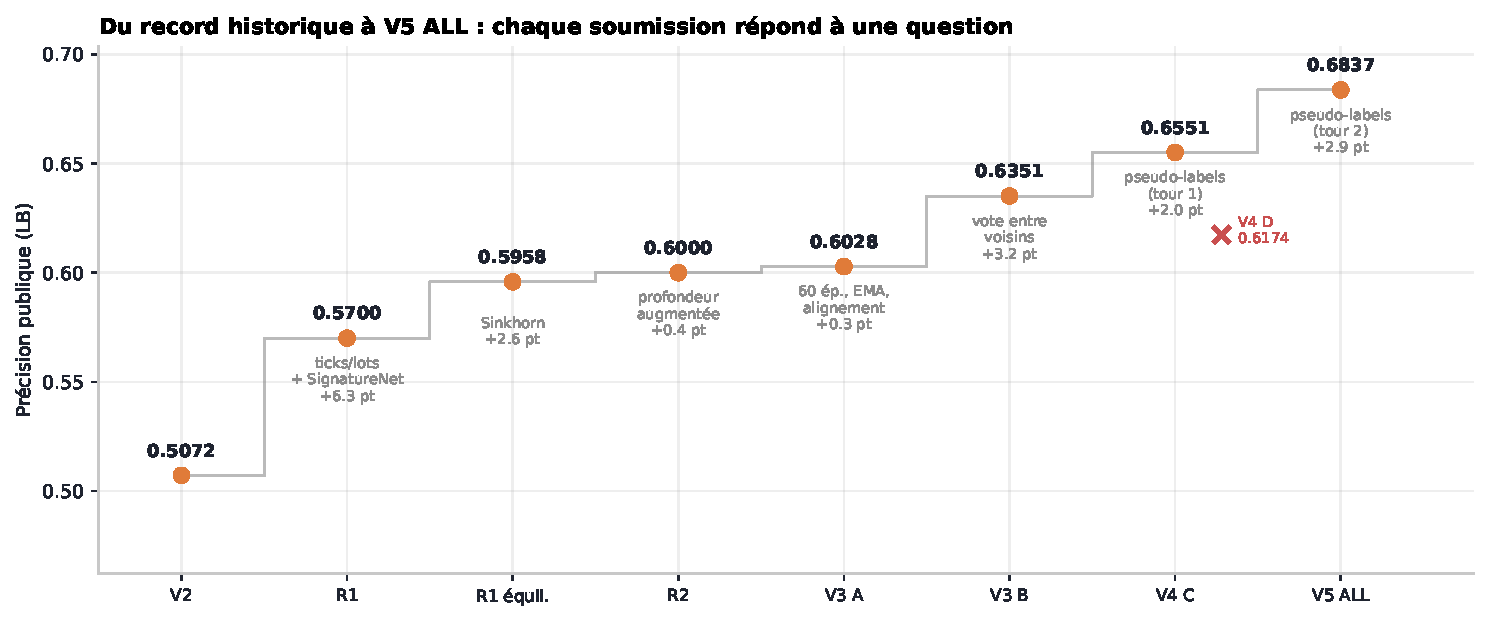
\includegraphics[width=\linewidth]{figures/v5_lb_journey.pdf}
\caption{Accuracy publique, soumission par soumission, avec le levier ajouté à chaque étape. La croix rouge est une soumission de contrôle (V4~D : V4~C sans les élèves). Section~\ref{sec:selftrain} pour V4 et V5.}
\label{fig:lb}
\end{figure}

\subsection{Contributions et honnêteté du propos}
\begin{enumerate}
\item Une couche de données \emph{validée} : alignement par \code{obs\_id}, contiguïté, renumérotation des ordres qui ne conserve que les égalités (section~\ref{sec:donnees}).
\item Une représentation en unités naturelles. Nous montrons formellement ce que la normalisation par médiane locale efface (section~\ref{sec:unites}).
\item Des tokens d'événements sans aucun seuil appris, et des statistiques de parcours d'ordres calculées de façon vectorisée et exacte (section~\ref{sec:ordres}), illustrés sur un exemple complet calculé par le code lui-même (section~\ref{sec:exemple}).
\item Un entonnoir de screening : utilité contre dérive, AUC adversariale, ajout et retrait réentraînés, intervalles appariés (section~\ref{sec:screening}).
\item SignatureNet, décrit équation par équation, avec un décompte exact de ses paramètres (section~\ref{sec:signaturenet}).
\item La correction de prior par Sinkhorn : dérivation, convergence, conditions de validité, effet observé (section~\ref{sec:sinkhorn}).
\item Un atlas de la donnée réelle (section~\ref{sec:atlas}) et une démonstration contrôlée de 25 modèles sur un même protocole, qui isole l'apport de la représentation : +16 points à architecture égale (section~\ref{sec:demo}).
\item L'auto-apprentissage transductif : filtre d'accord entre deux lectures du professeur, quota équilibré par titre, deux tours, soumissions de contrôle et analyse de la contamination des mesures internes (section~\ref{sec:selftrain}).
\end{enumerate}
\noindent Ce que ce document \emph{ne} prétend \emph{pas}. Les $+6{,}3$ points du premier run mêlent représentation, architecture et ensemble : un seul score public ne permet pas de les séparer, et la démonstration de la section~\ref{sec:demo} ne les sépare qu'en interne. Les gains de validation ne sont pas des gains de test. L'équilibrage suppose un test équilibré entre titres et utilise les entrées du test, comme le vote entre voisins et l'auto-apprentissage : leur conformité au règlement est à vérifier. Les mesures internes des élèves V4/V5 sont contaminées par leur professeur : seul le LB y tranche. Enfin, les résultats synthétiques cités en annexe valident le logiciel, jamais la performance.

\section{Le problème et ses données}\label{sec:probleme}

\subsection{Notation}
Le jeu d'entraînement contient $N_{\text{tr}}=160\,800$ fenêtres, et le test $N_{\text{te}}=81\,600$. Une fenêtre $W$ est une suite ordonnée
\begin{equation}
W=(e_1,\dots,e_L),\qquad L=100,
\end{equation}
et chaque événement est un n-uplet
\begin{equation}
e_t=\big(v_t,\;o_t,\;a_t,\;s_t,\;p_t,\;b_t,\;\alpha_t,\;q^b_t,\;q^a_t,\;\tau_t,\;f_t\big)
\end{equation}
où :
\begin{itemize}
\item $v_t\in\{0,\dots,5\}$ est la \emph{venue}, c'est-à-dire la place où l'événement a lieu ;
\item $o_t$ est l'identifiant anonymisé de l'ordre, local à la fenêtre ;
\item $a_t\in\{A,D,U\}$ est l'action : ajout, suppression ou mise à jour ;
\item $s_t\in\{A,B\}$ est le côté : vente (ask) ou achat (bid) ;
\item $p_t$ est le prix de l'ordre concerné ;
\item $b_t$ et $\alpha_t$ sont le meilleur bid et le meilleur ask du carnet \emph{agrégé entre places}, après l'événement ;
\item $q^b_t$ et $q^a_t$ sont les quantités affichées à ces meilleures limites ;
\item $\tau_t\in\{0,1\}$ indique si une suppression ou une mise à jour résulte d'une transaction ;
\item $f_t$ est la variation signée de volume associée à l'événement.
\end{itemize}
La cible est $y\in\{0,\dots,K-1\}$, avec $K=24$.

\paragraph{Recentrage.} Les prix sont fournis \emph{décalés} par le premier bid de la fenêtre : $p_t\leftarrow p_t-b_1$, et de même pour $b_t$ et $\alpha_t$. Le niveau absolu du prix est donc inconnu. Un offset proche de zéro n'est pas un prix : diviser par lui n'a pas de sens.

\paragraph{Carnet agrégé.} $(b_t,\alpha_t,q^b_t,q^a_t)$ décrivent le carnet consolidé entre places. La venue $v_t$ décrit l'événement, pas un carnet séparé. Deux événements consécutifs sur des places différentes s'appliquent donc au même état agrégé.

\subsection{Structure hiérarchique : titres, jours, fenêtres}\label{sec:hierarchie}
D'après la description du challenge rapportée par l'auteur, il y a 20 fenêtres par titre et par jour. Le train couvre donc
\[
D_{\text{tr}}=\frac{160\,800}{24\times 20}=335\ \text{jours par titre},\qquad D_{\text{te}}=\frac{81\,600}{24\times 20}=170 .
\]
Cette structure a une conséquence centrale (section~\ref{sec:dependance}). Écrivons une statistique $x$ d'une fenêtre $w$ du titre $c$ le jour $d$ :
\begin{equation}
x_{c,d,w}=\mu_c+\eta_{c,d}+\varepsilon_{c,d,w},\qquad \eta_{c,d}\sim(0,\sigma^2_\eta),\ \varepsilon\sim(0,\sigma^2_\varepsilon).
\label{eq:hier}
\end{equation}
$\mu_c$ est la signature durable du titre. $\eta_{c,d}$ est un effet de journée : niveau de prix, volatilité, profondeur du jour. $\varepsilon$ est la variation propre à la fenêtre. Un classifieur peut reconnaître $c$ grâce à $\mu_c$, ce qui transfère dans une autre période. Il peut aussi le reconnaître grâce à $\eta_{c,d}$, s'il a vu d'autres fenêtres du même jour. Ce second mécanisme ne transfère pas : les jours du test sont nouveaux.

\subsection{Changement de période}
Les périodes de train et de test diffèrent, et aucune date n'est disponible par observation. Nous distinguons trois formes de décalage, que la suite du document traite séparément :
\begin{enumerate}
\item \textbf{covariate shift} : $p_{\text{te}}(x)\neq p_{\text{tr}}(x)$. Par exemple, les carnets sont moins profonds dans le test ;
\item \textbf{décalage de la relation} : $p_{\text{te}}(y\mid x)\neq p_{\text{tr}}(y\mid x)$. La même profondeur ne désigne plus les mêmes titres ;
\item \textbf{décalage de prior des prédictions} : même si $p_{\text{te}}(y)$ est uniforme, un covariate shift peut rendre la répartition des \emph{prédictions} très non uniforme. C'est ce que corrige la section~\ref{sec:sinkhorn}.
\end{enumerate}

\section{Avant / maintenant : deux pipelines côte à côte}\label{sec:avantapres}

Cette section sert de carte. Les deux schémas suivent une fenêtre de la lecture du CSV jusqu'à la soumission. Les numéros de section renvoient aux définitions précises.

\tikzset{
  stage/.style={draw, rounded corners=2pt, align=left, font=\scriptsize, inner sep=3pt, text width=#1},
  stage/.default=5.6cm,
  oldst/.style={stage=5.6cm, fill=old!8, draw=old!70},
  newst/.style={stage=5.6cm, fill=new!8, draw=new!70},
  arr/.style={-{Stealth[length=2mm]}, thick, gray!70},
  lbl/.style={font=\scriptsize\bfseries, text=gray!80!black}
}

\begin{figure}[p]
\centering
\begin{tikzpicture}[node distance=3.2mm]
% ---------- AVANT ----------
\node[font=\bfseries, text=old] (h1) {AVANT (Reaction R1/R2, référence V2)};
\node[oldst, below=of h1] (o1) {\textbf{1. Lecture} \\ CSV → fenêtres de 100 lignes. Catégories one-hot (R2) ou embeddings de dim.~8 (V2). Tailles négatives remplacées par 0.};
\node[oldst, below=of o1] (o2) {\textbf{2. Échelles locales} \\ $s^\star=\Med(\text{spread}>0)$, $d^\star=\Med(\text{profondeur})$, $f^\star=\Med|f|$ \emph{de la fenêtre}. \\ Toutes les grandeurs sont divisées par ces médianes : $\log(1+\text{spread}/s^\star)$, $\operatorname{asinh}(\Delta\text{mid}/s^\star)$, etc.};
\node[oldst, below=of o2] (o3) {\textbf{3. Canaux par événement} (19 réels) \\ spread, trajectoire et variation du mid, position du prix, imbalance, profondeur relative et variation, flux relatif et variation, ordre déjà vu, même ordre que l'événement précédent, fraction invalide, quote-flow, 6 historiques d'ordre.};
\node[oldst, below=of o3] (o4) {\textbf{4. Contexte de fenêtre} \\ moyennes et écarts-types des canaux, log-spread, log-profondeur, échelle de flux, offset du mid, réactions régularisées vers un prior.};
\node[oldst, below=of o4] (o5) {\textbf{5. Split} \\ train / valid / stress / audit. Stress = queue \old{\textbf{haute}} de profondeur, codée en dur (\code{STRESS\_TAIL='high'}).};
\node[oldst, below=of o5] (o6) {\textbf{6. Modèle} \\ BiGRU (48) → pooling moyenne + max → 64 \\ contexte MLP → 32 \\ fusion 96 → 64 → 24 \quad($\approx$ 39\,k paramètres). \\ Option : auxiliaire de mouvement du mid.};
\node[oldst, below=of o6] (o7) {\textbf{7. Sélection} \\ meilleure époque en validation aléatoire ; LR fixe ; 24 à 60 époques.};
\node[oldst, below=of o7] (o8) {\textbf{8. Sortie} \\ ensemble de seeds / variantes (V2), $\arg\max$.};
\node[font=\scriptsize, below=1mm of o8, text width=5.6cm, align=center] (os) {valid R1 $\approx 0{,}55$ — LB record $\mathbf{0{,}5072}$ (V2)};
\foreach \a/\b in {o1/o2,o2/o3,o3/o4,o4/o5,o5/o6,o6/o7,o7/o8} \draw[arr] (\a) -- (\b);

% ---------- MAINTENANT ----------
\node[font=\bfseries, text=new, right=1.4cm of h1] (h2) {MAINTENANT (Signature Lab)};
\node[newst, below=of h2] (n1) {\textbf{1. Cache brut validé} (§\ref{sec:donnees}) \\ contiguïté et unicité des \code{obs\_id}, labels alignés \emph{par identifiant}, $o_t\mapsto$ rang de 1\textsuperscript{re} apparition, catégories avec modalité inconnue, \new{tick estimé puis vérifié}. Valeurs brutes conservées, y compris les tailles négatives.};
\node[newst, below=of n1] (n2) {\textbf{2. Unités naturelles} (§\ref{sec:unites}) \\ prix en \new{ticks} $\tick=0{,}01$ ; quantités en \new{lots} $\lot=100$. \\ spread $S_t\in\N$, $\Delta$mid en demi-ticks, distance au meilleur prix \emph{de son côté} $D_t$, flux $f_t/\lot$.};
\node[newst, below=of n2] (n3) {\textbf{3. Événement = 11 tokens + 11 canaux} (§\ref{sec:ordres}) \\ action, côté, trade, venue, zone de prix $D_t$, taille en lots, spread en ticks, $\Delta$mid, occurrence de l'ordre, action précédente \emph{du même ordre}, signe du flux. \\ \new{Seuils fixés a priori} ; canaux continus relatifs et en unités naturelles.};
\node[newst, below=of n3] (n4) {\textbf{4. Blocs de fenêtre} (§\ref{sec:blocs}) \\ 11 blocs nommés (\code{ticks}, \code{lots}, \code{position}, \code{orders}, \code{levels}…), cache par empreinte du code. \\ \new{Entonnoir} : utilité $\eta^2$ / dérive KS → AUC adversariale → ajout réentraîné → retrait réentraîné (§\ref{sec:screening}).};
\node[newst, below=of n4] (n5) {\textbf{5. Split} (§\ref{sec:protocole}) \\ audit tiré \emph{en premier} (seed dédiée) ; stress = queue \new{\textbf{basse}}, orientée par la médiane test ; valid ; fit.};
\node[newst, below=of n5] (n6) {\textbf{6. SignatureNet} (§\ref{sec:signaturenet}) \\ $\sum$ embeddings + linéaire + position → 2 conv. dilatées → 2 attentions avec biais $\beta_h\cdot[\text{même ordre}]$ → pooling attention/moy/max \\ ⊕ contexte 79 → 128 → 64 ; fusion 160 → 96 → 24 \quad (342\,913 paramètres).};
\node[newst, below=of n6] (n7) {\textbf{7. Entraînement et sélection} (§\ref{sec:entrainement}) \\ AdamW, warmup + cosinus, 40 époques ; époque choisie en valid ; \new{configs comparées sur le stress équilibré} ; refit sur tous les labels.};
\node[newst, below=of n7] (n8) {\textbf{8. Sortie} (§\ref{sec:sinkhorn}) \\ moyenne de 2 configs $\times$ 2 seeds → \new{équilibrage de Sinkhorn} (coefficient $w_c$ par titre) → $\arg\max$.};
\node[font=\scriptsize, below=1mm of n8, text width=5.6cm, align=center] (ns) {valid 0,85 (non prédictif) — LB $\mathbf{0{,}5700}$ puis $\mathbf{0{,}5958}$};
\foreach \a/\b in {n1/n2,n2/n3,n3/n4,n4/n5,n5/n6,n6/n7,n7/n8} \draw[arr] (\a) -- (\b);
\foreach \a/\b in {o1/n1,o2/n2,o3/n3,o4/n4,o5/n5,o6/n6,o7/n7,o8/n8} \draw[dashed, gray!50] (\a.east) -- (\b.west);
\end{tikzpicture}
\caption{Les deux pipelines, étape par étape. Les pointillés relient les étapes homologues.}
\label{fig:avantapres}
\end{figure}

\subsection{Comparaison détaillée par étape}

\begin{longtable}{>{\raggedright\arraybackslash}p{2.2cm}>{\raggedright\arraybackslash}p{4.6cm}>{\raggedright\arraybackslash}p{4.6cm}>{\raggedright\arraybackslash}p{3.2cm}}
\toprule
\textbf{Étape} & \textbf{Avant} & \textbf{Maintenant} & \textbf{Pourquoi}\\
\midrule\endhead
Spread & $\log(1+S/s^\star)$, $s^\star$ = médiane locale : un spread constant à 1 tick donne $\log 2$, comme un spread constant à 5 ticks & $S_t=(\alpha_t-b_t)/\tick\in\{0,1,2,\dots\}$ ; parts de fenêtre à 1, 2, 3--4, $\ge5$ ticks ; token & Le régime de tick est une signature (η² $\approx 0{,}5$, KS $\approx 0{,}02$, §\ref{sec:resultats})\\
Prix de l'événement & $\operatorname{asinh}((p-m)/s^\star)$, relatif au \emph{mid} & $D_t$ = distance en ticks au meilleur prix \emph{de son côté} : dans le spread / au meilleur / 1 / 2 / 3--5 / $>5$ & Un ordre « 2 ticks derrière le meilleur ask » décrit un comportement, quelle que soit la largeur du spread\\
Quantités & $\log(1+q/d^\star)$ & $q/\lot$ (lots), parts de lots ronds / odd lots / mixtes ; token de taille & Les conventions de lot sont propres au titre ; leur dérive est mesurée explicitement\\
Ordres & « déjà vu », « même que précédent », écart, âge, dernière action & + rang de 1\textsuperscript{re} apparition, première action, \emph{action précédente du même ordre}, nombre d'événements de l'ordre ; relation « même ordre » dans l'attention & Le cycle de vie A→U→D d'un ordre est une empreinte, même tronquée\\
Catégories & one-hot ou embedding dim.~8 & tokens additionnés en dim.~96, modalité 0 = inconnu & Toutes les entrées discrètes sont traitées pareil\\
Tailles $<0$ & remplacées par 0 & conservées brutes ; NaN dans les grandeurs dérivées ; fréquence mesurée & Une convention ne doit pas créer de fausse valeur\\
Contexte & mean/std de canaux relatifs & 11 blocs nommés (\textasciitilde 200 colonnes), retenus par l'entonnoir & Hypothèses testables une par une\\
Stress & queue haute & queue basse, orientée vers le test (transductif, consigné) & Le test est moins profond : médiane $\log(1+\text{prof.}/\lot)$ de 1,84 (train) contre 1,70 (test)\\
Encodeur & BiGRU 48 & conv.\ dilatées + attention relationnelle & Motifs locaux et relations longues séparés\\
Sélection & valid aléatoire & stress équilibré + indicateurs sans labels & Valid 0,85 contre LB 0,57\\
Sortie & $\arg\max$ & Sinkhorn puis $\arg\max$ & Prédictions biaisées vers les titres peu profonds\\
\bottomrule
\caption{Comparaison détaillée. $s^\star$, $d^\star$ : médianes locales de la fenêtre.}
\end{longtable}

\section{Couche de données : un cache brut validé}\label{sec:donnees}

Cette section décrit \code{cfm/io.py}. Son principe : aucune transformation \emph{statistique} ici. On lit, on vérifie, on type et on aligne. Ce qui est calculé ensuite dépend de ce cache, et toute incohérence doit y être arrêtée.

\subsection{Contrats vérifiés à la lecture}
Le CSV est lu par blocs de $20\,000$ fenêtres ($2\cdot10^6$ lignes). Pour chaque bloc de $m$ fenêtres, on remodèle les identifiants en matrice $I\in\Z^{m\times L}$ et on exige :
\begin{equation}
\forall i,\ \forall t:\ I_{i,t}=I_{i,1}.
\end{equation}
Autrement dit, chaque groupe de 100 lignes consécutives porte un seul \code{obs\_id}. Comme la taille de bloc est un multiple de 100 et que le nombre total de lignes l'est aussi (vérifié en première passe), aucune fenêtre ne peut chevaucher deux blocs. On vérifie ensuite l'unicité des \code{obs\_id} sur tout le fichier, puis l'égalité \emph{ensembliste} entre les identifiants de \code{X\_train} et de \code{y\_train}. Les labels sont alignés \emph{par identifiant} :
\begin{equation}
y_i=\texttt{y\_train}[\texttt{obs\_id}=I_{i,1}],
\end{equation}
et non par position de ligne : un \code{y\_train} mélangé donne le même résultat. C'est l'objet d'un test de contrat.

\subsection{Catégories}
Les catégories sont normalisées : chaîne, espaces retirés, majuscules, suffixe « .0 » retiré. Elles sont ensuite codées avec des vocabulaires \emph{fixes} pour action, côté et trade : $A\mapsto1$, $D\mapsto2$, $U\mapsto3$ ; $A\mapsto1$, $B\mapsto2$ ; \code{FALSE}$\mapsto1$, \code{TRUE}$\mapsto2$. Le vocabulaire des venues est construit sur le train uniquement, sans labels. Toute valeur hors vocabulaire reçoit le code $0$ (« inconnu »), et son nombre d'occurrences par partition est consigné dans \code{meta.json}.

\subsection{Identité des ordres : ne garder que les égalités}
Les \code{order\_id} sont des entiers anonymisés, locaux à la fenêtre. La distance numérique entre deux identifiants n'a pas de sens économique établi. Seule l'égalité en a un : « c'est le même ordre ». On remplace donc $o_t$ par son \emph{rang de première apparition}.

\begin{definition}[Rang de première apparition]
Pour une fenêtre $(o_1,\dots,o_L)$, notons $\phi(t)=\min\{u\le t: o_u=o_t\}$ la première position de l'ordre de l'événement $t$. On pose
\begin{equation}
\rho(t)=\big|\{\phi(u):u\le t\}\big|-1,
\end{equation}
c'est-à-dire le nombre d'ordres distincts apparus avant celui de $t$. Les identifiants manquants reçoivent chacun un rang propre : ils ne sont jamais égaux entre eux.
\end{definition}

\begin{proposition}[Invariance par renumérotation]\label{prop:bij}
Soit $\pi$ une bijection quelconque de l'ensemble des identifiants. Alors la suite des rangs calculée sur $(\pi(o_1),\dots,\pi(o_L))$ est identique à celle calculée sur $(o_1,\dots,o_L)$.
\end{proposition}
\begin{proof}
$\phi$ ne dépend que des égalités $o_u=o_t$, et $\pi$ les préserve puisqu'elle est injective. $\rho$ est une fonction de $\phi$ seulement.
\end{proof}
\noindent Conséquence : aucun composant du modèle ne peut exploiter la valeur des identifiants. Le test de contrat applique des renumérotations aléatoires et vérifie l'égalité exacte.

\paragraph{Calcul vectorisé.} Pour un bloc de $m$ fenêtres, on forme une clé entière unique par couple (fenêtre, identifiant) :
\begin{equation}
\kappa_{i,t}=i\cdot2^{32}+(\tilde o_{i,t}+2^{31}),\qquad \tilde o_{i,t}=\begin{cases}o_{i,t}&\text{si défini}\\-1-t&\text{sinon,}\end{cases}
\end{equation}
puis \code{np.unique(return\_index, return\_inverse)} donne, pour chaque clé distincte, sa première position $\phi$. Un tri lexicographique par (fenêtre, $\phi$) suivi d'un compteur remis à zéro à chaque nouvelle fenêtre donne $\rho$. Le coût est $O(mL\log(mL))$, sans boucle Python.

\subsection{Estimation et vérification du tick}
\begin{algo}[H]
\caption{Estimation du tick (\code{estimate\_tick})}
\begin{algobox}
\item Lire les $2\cdot10^6$ premières lignes du train. Calculer les spreads $\alpha_t-b_t$, arrondis à $10^{-6}$, strictement positifs.
\item Garder les valeurs dont la fréquence est d'au moins $1\,\%$ des spreads positifs. Poser $\hat\tick$ = la plus petite d'entre elles.
\item Pour $x\in\{p,b,\alpha\}$, mesurer la part hors grille : $\frac1n\sum\ind{|x/\hat\tick-\operatorname{round}(x/\hat\tick)|>10^{-3}}$.
\item \code{grid\_ok} $\iff$ part hors grille $<1\,\%$ pour $b$ et $\alpha$. Sinon, avertir : les blocs en ticks deviennent des approximations.
\end{algobox}
\end{algo}
\noindent Le recentrage soustrait $b_1$, qui est lui-même sur la grille, donc les offsets restent des multiples entiers de $\tick$. C'est ce qui rend les quantités « en ticks » \emph{exactement} entières (modulo l'arrondi flottant), alors qu'une division par une médiane ne l'est pas.

\subsection{Disposition du cache}
\begin{center}\small
\begin{tabular}{lll}
\toprule
Fichier & Forme, type & Contenu\\
\midrule
\code{\{split\}\_num.npy} & $(n,100,6)$ float32 & $p,b,\alpha,q^b,q^a,f$ bruts (rien n'est écrêté)\\
\code{\{split\}\_cat.npy} & $(n,100,4)$ int8 & venue, action, côté, trade ; 0 = inconnu\\
\code{\{split\}\_oid.npy} & $(n,100)$ int8 & $\rho(t)$\\
\code{\{split\}\_ids.npy} & $(n,)$ int64 & \code{obs\_id} dans l'ordre du fichier\\
\code{train\_y.npy} & $(n,)$ int16 & indice de classe dans \code{meta['classes']}\\
\bottomrule
\end{tabular}
\end{center}
Le cache est lié à l'empreinte des fichiers sources (chemin, taille). Un cache construit sur d'autres CSV est refusé.

\section{Atlas des données}\label{sec:atlas}

Cette section montre la donnée réelle avant toute modélisation. Les figures viennent du notebook \code{v\_demo/CFM\_demo\_features}, exécuté sur Kaggle. Le test n'a pas de labels. Pour le découper par titre, on utilise le titre \emph{prédit} par V3~B (0,635 au LB) : les barres « test » sont donc approximatives, d'autant plus pour les titres que le modèle confond.

\subsection{Une fenêtre, vue de près}
\begin{figure}[H]\centering
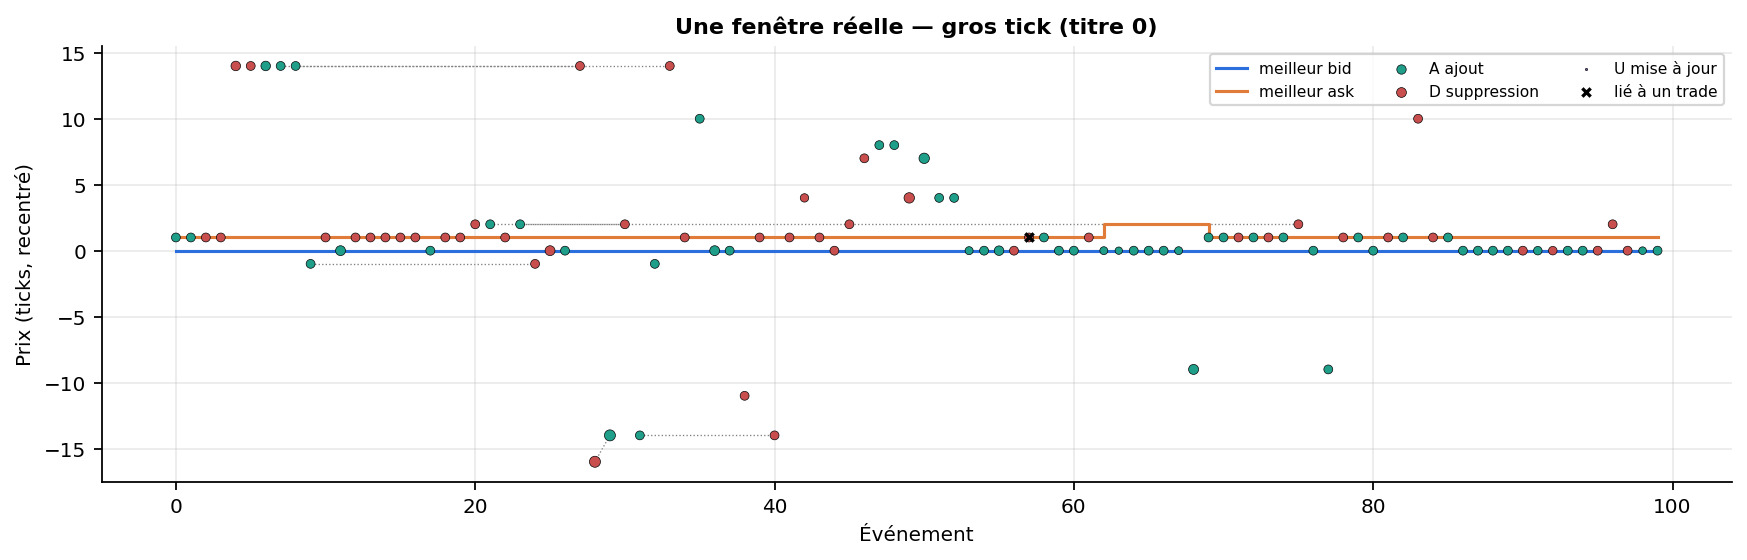
\includegraphics[width=.9\linewidth]{figures/demo_d1_window_big.png}\\[4pt]
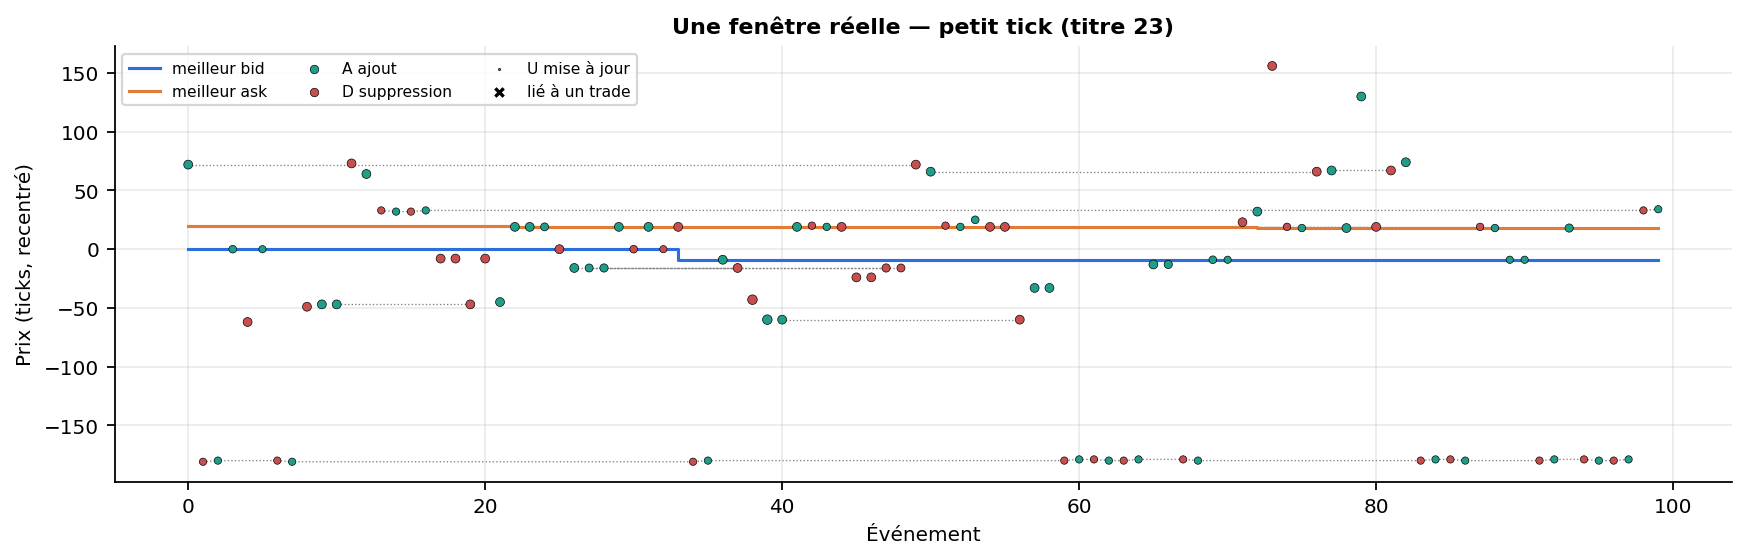
\includegraphics[width=.9\linewidth]{figures/demo_d1_window_small.png}
\caption{Deux vraies fenêtres de 100 événements, prix en ticks recentrés sur le mid initial. En haut, un titre à \emph{gros} tick (titre 0) : le meilleur bid et le meilleur ask sont collés à un tick d'écart et ne bougent presque pas, et les ordres se placent sur quelques niveaux entiers. En bas, un titre à \emph{petit} tick (titre 23) : les ordres s'étalent sur $\pm150$ ticks et le spread vaut plusieurs dizaines de ticks. Exprimées en multiples d'une médiane locale, ces deux fenêtres se ressembleraient bien davantage. C'est l'argument visuel de la section~\ref{sec:unites}.}
\label{fig:atlas-window}\end{figure}

\begin{figure}[H]\centering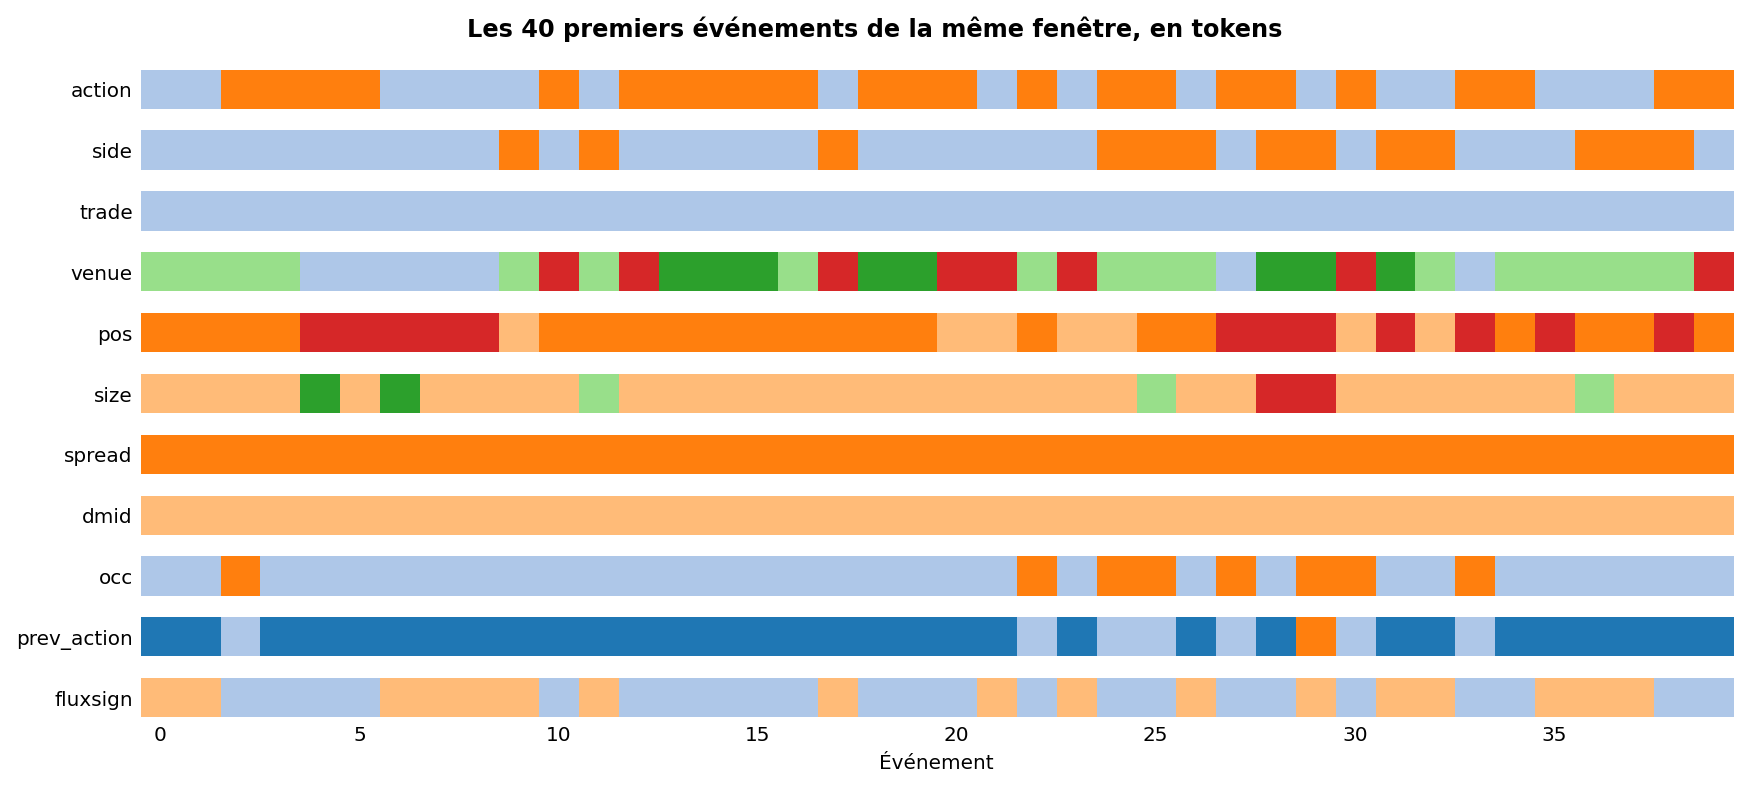
\includegraphics[width=.95\linewidth]{figures/demo_d1_tokens.png}
\caption{Les 40 premiers événements d'une fenêtre, vus par le réseau : une ligne par token (action, côté, trade, venue, position, taille, spread, $\Delta$mid, occurrence, action précédente du même ordre, signe du flux), une couleur par valeur. Certaines lignes sont presque constantes dans une fenêtre (spread, $\Delta$mid) : elles portent le \emph{régime}. D'autres changent à chaque événement (action, venue, occurrence) : elles portent la \emph{dynamique}.}
\end{figure}

\begin{figure}[H]\centering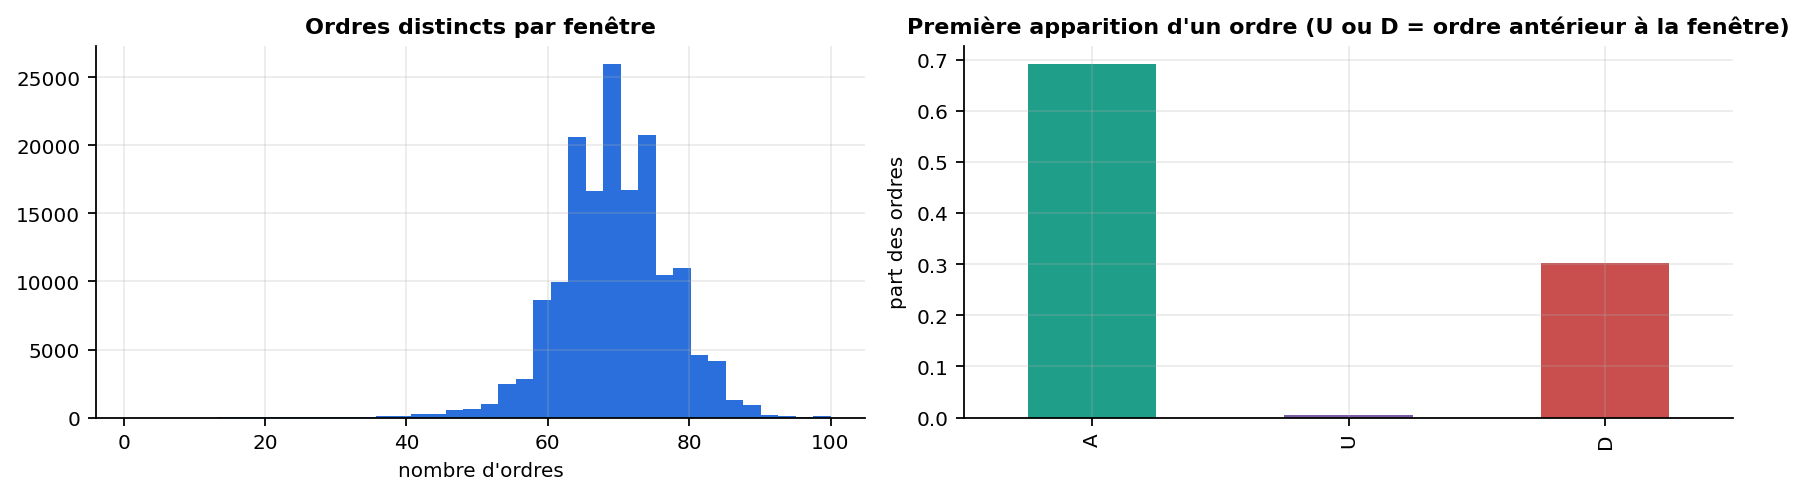
\includegraphics[width=.8\linewidth]{figures/demo_d1_orders.png}
\caption{Ordres par fenêtre. À gauche, une fenêtre de 100 événements touche environ 70 ordres distincts : la plupart n'apparaissent qu'une fois, mais un tiers environ reviennent. À droite, la première apparition d'un ordre est un ajout dans 70\,\% des cas, et une suppression dans 30\,\% : ces ordres ont été placés \emph{avant} la fenêtre. D'où l'intérêt des tokens d'occurrence et d'action précédente du même ordre (section~\ref{sec:ordres}).}
\end{figure}

\subsection{Ce qui distingue les titres}
\begin{figure}[H]\centering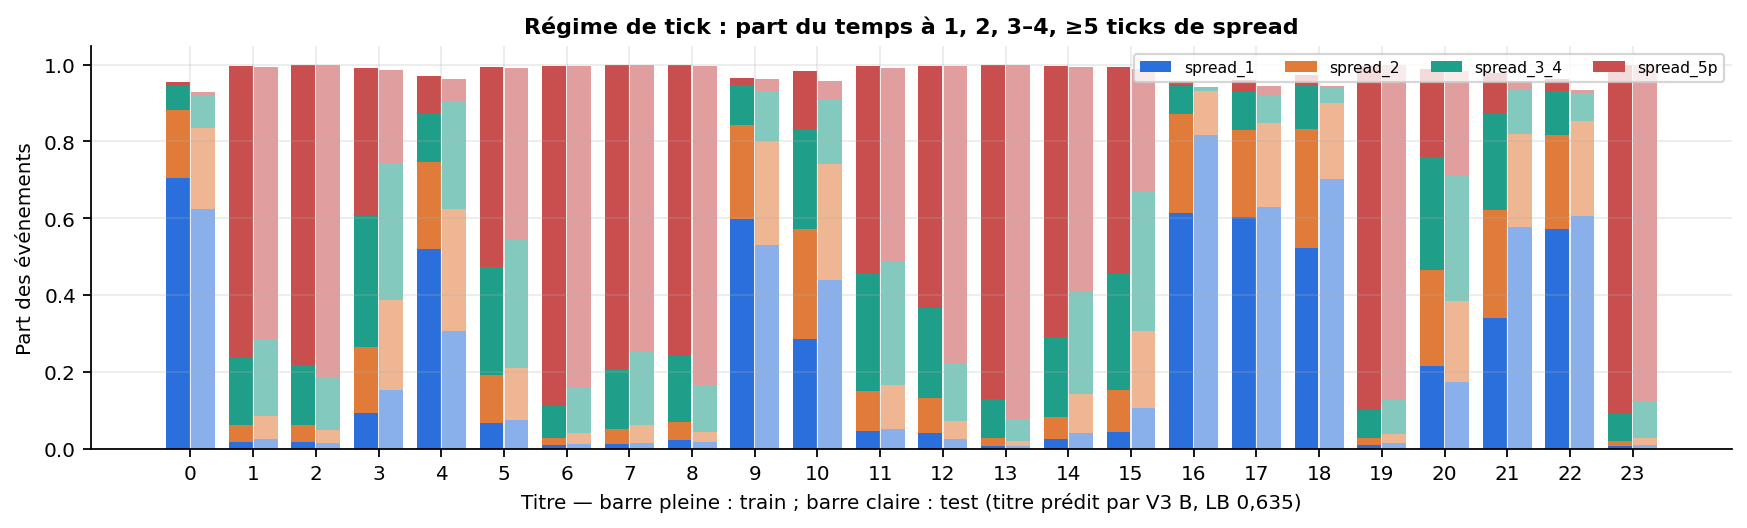
\includegraphics[width=\linewidth]{figures/demo_d2_ticks.png}
\caption{Part du temps passé avec un spread de 1, 2, 3--4 ou au moins 5 ticks, par titre (barre pleine : train ; barre claire : test). Les titres se rangent en deux familles nettes : ceux qui vivent à un tick (0, 9, 16, 17, 22\ldots) et ceux dont le spread dépasse presque toujours 5 ticks. Les barres train et test sont presque identiques : c'est la signature stable par excellence ($\mathrm{KS}\approx0{,}02$, section~\ref{sec:resultats}).}
\label{fig:atlas-ticks}\end{figure}

\begin{figure}[H]\centering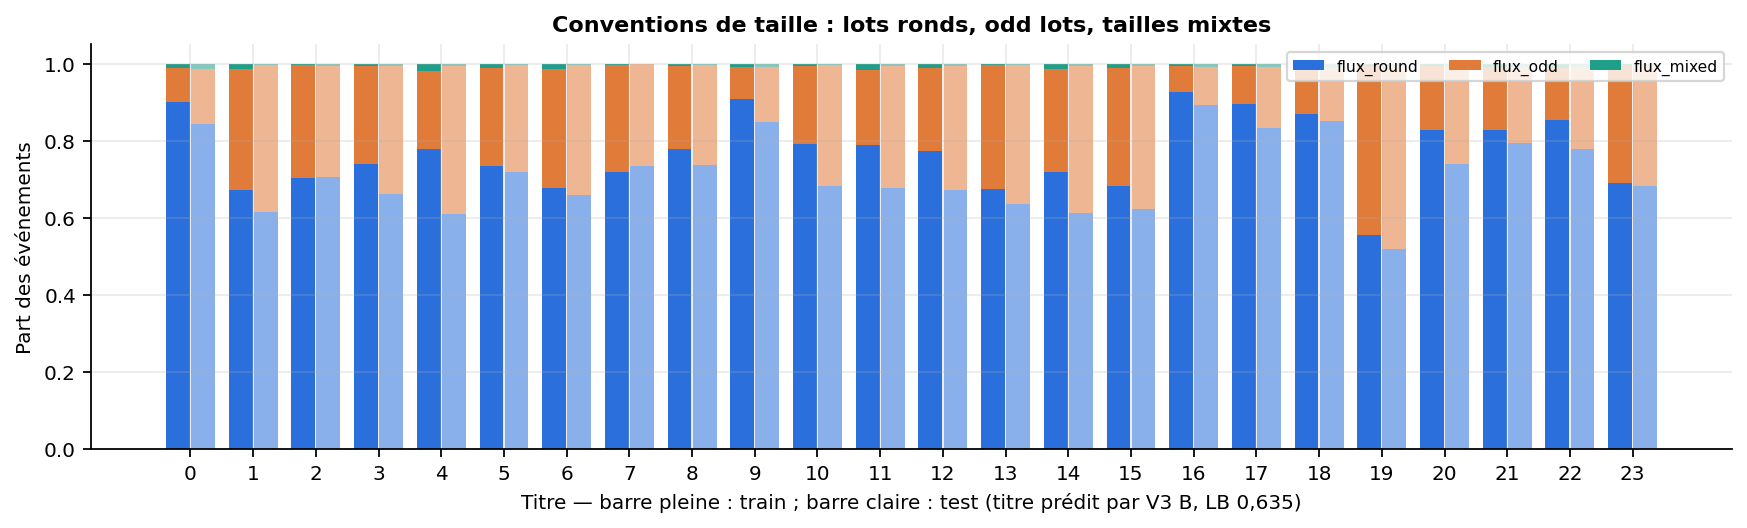
\includegraphics[width=\linewidth]{figures/demo_d2_lots.png}
\caption{Répartition du flux entre lots ronds (multiples de 100), odd lots et tailles mixtes. Les titres se distinguent nettement par leurs conventions de taille. Mais sur la période test, la part d'odd lots augmente pour presque tous les titres. C'est un premier indice de prix plus élevés (section~\ref{sec:aug}).}
\end{figure}

\begin{figure}[H]\centering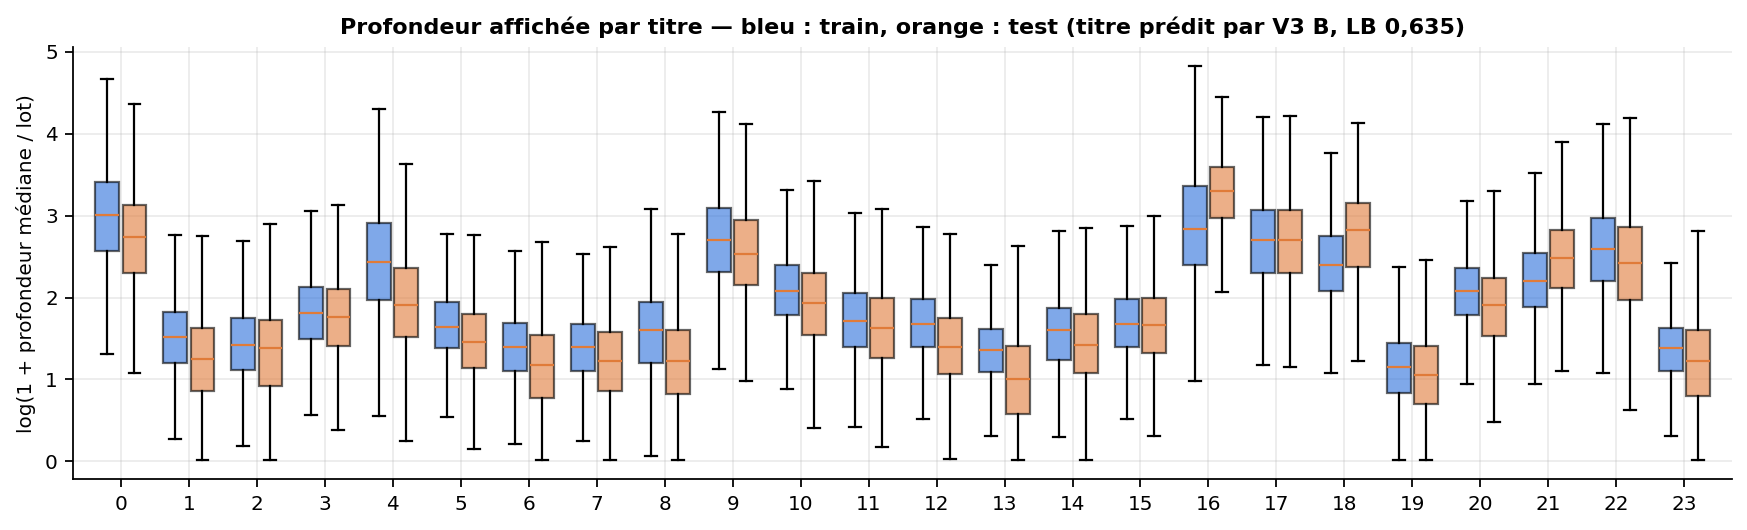
\includegraphics[width=\linewidth]{figures/demo_d2_depth.png}
\caption{Profondeur médiane du carnet (log, en lots) par titre, train en bleu et test en orange. Elle sépare bien les titres, mais elle \emph{baisse} sur le test pour la majorité d'entre eux. C'est le piège de régime de la section~\ref{sec:screening}, et la motivation de l'augmentation et de l'alignement de profondeur.}
\label{fig:atlas-depth}\end{figure}

\begin{figure}[H]\centering
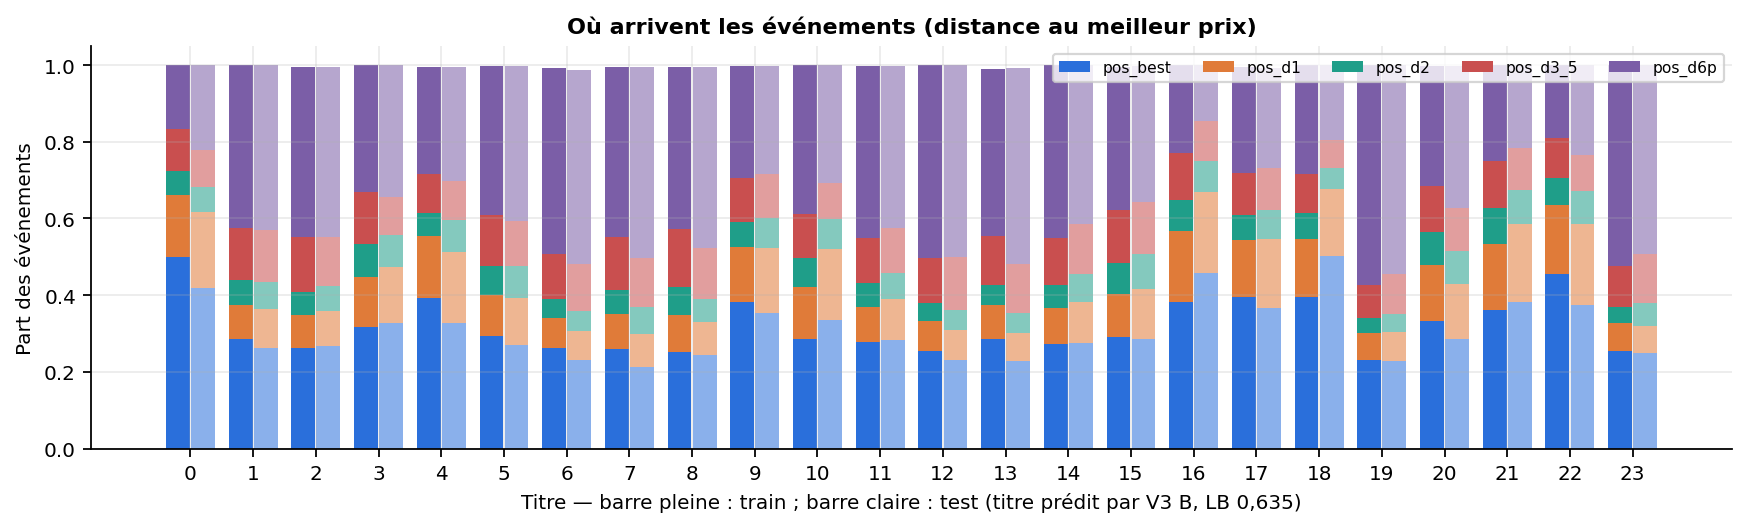
\includegraphics[width=\linewidth]{figures/demo_d2_position.png}\\[4pt]
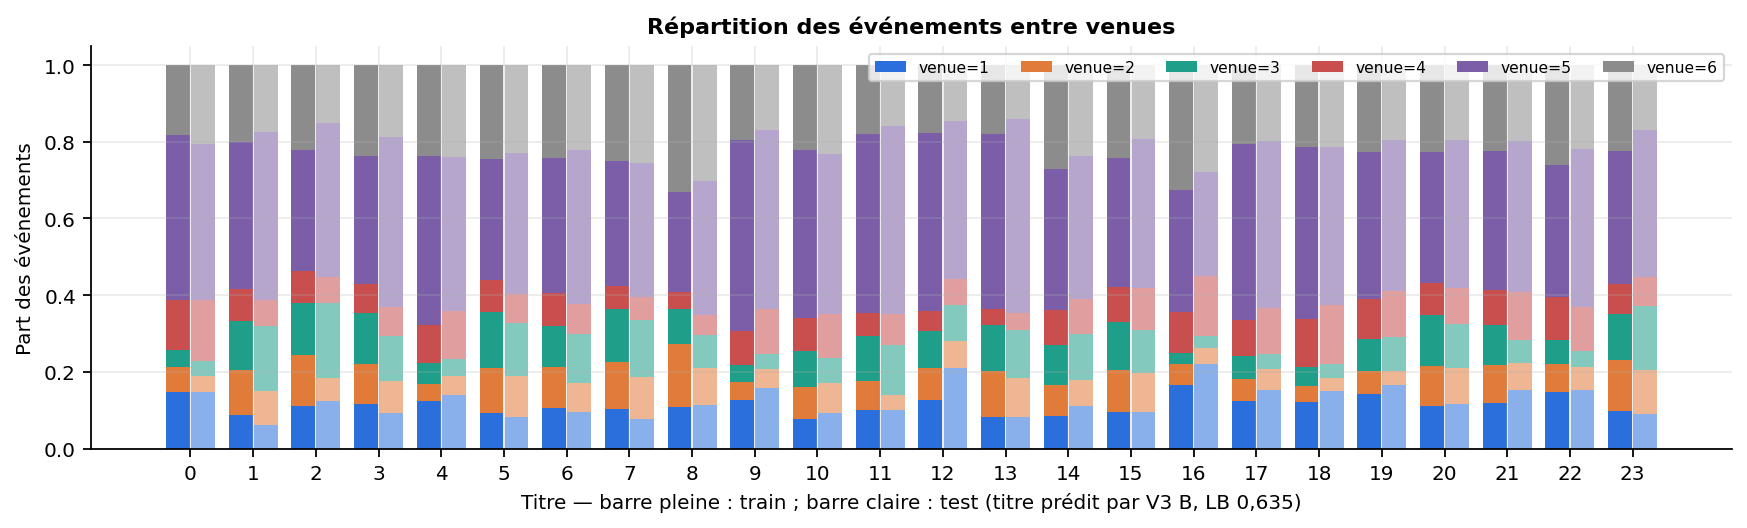
\includegraphics[width=\linewidth]{figures/demo_d2_venues.png}
\caption{En haut, la distance des événements au meilleur prix (au meilleur, à 1, 2, 3--5, 6 ticks et plus). En bas, la répartition entre venues. Les deux varient d'un titre à l'autre et restent stables entre train et test : ce sont des signatures secondaires, mais fiables.}
\end{figure}

\begin{figure}[H]\centering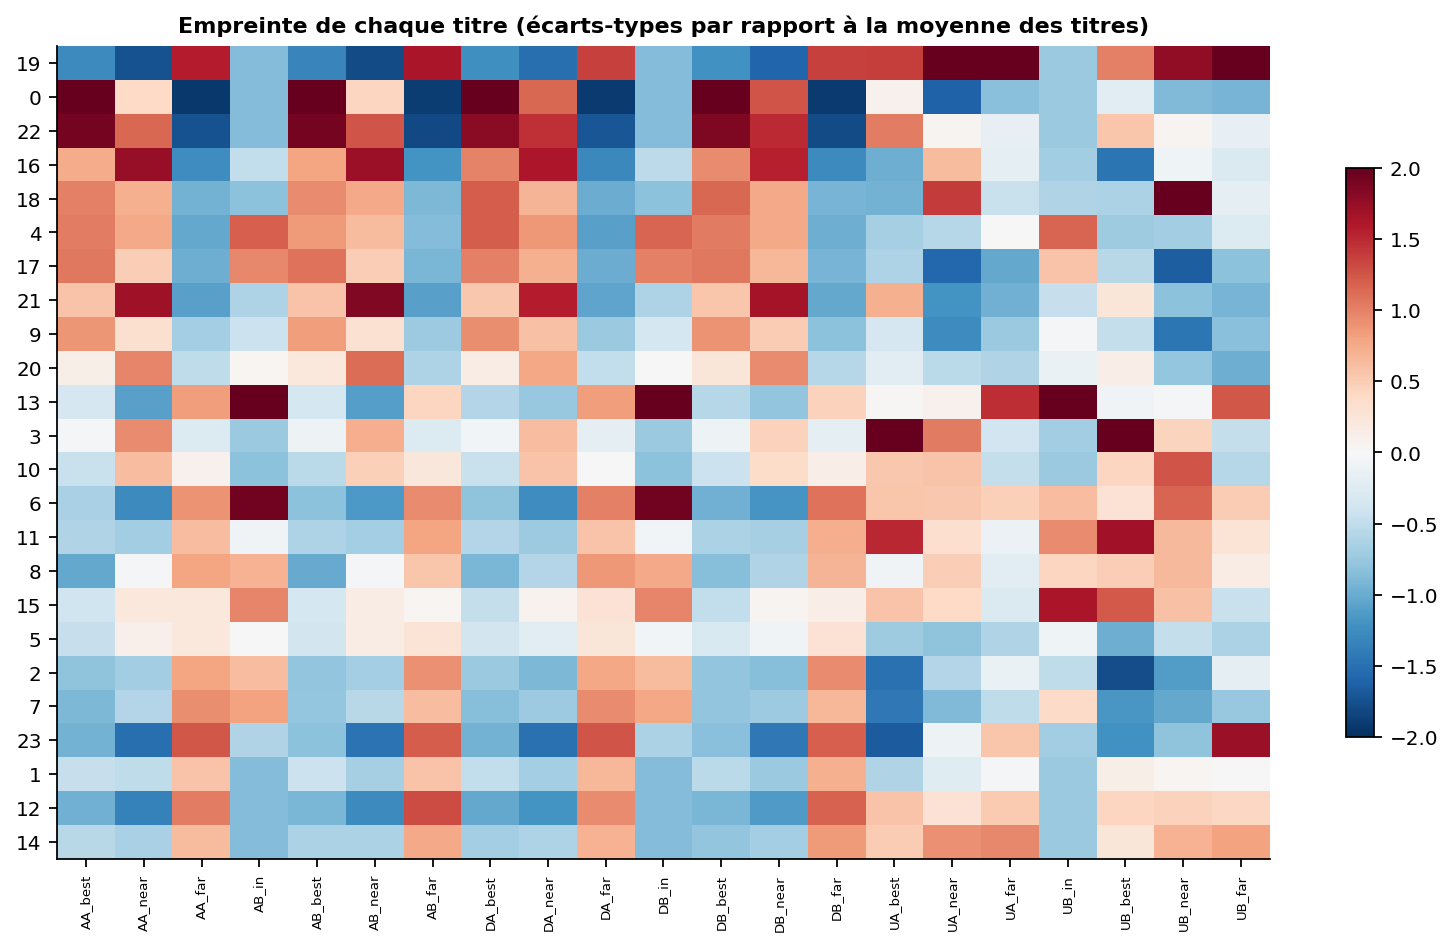
\includegraphics[width=.85\linewidth]{figures/demo_d2_token_fingerprint.png}
\caption{L'empreinte « sac de mots » de chaque titre : fréquence des combinaisons action $\times$ côté $\times$ zone de prix, en écarts-types par rapport à la moyenne des titres. Les titres sont réordonnés par ressemblance. Des blocs de titres aux empreintes voisines apparaissent, par exemple 0 et 22, et ces familles se retrouvent dans les matrices de confusion (figure~\ref{fig:confusion}, famille $\{0,9,17,22\}$).}
\end{figure}

\subsection{Ce qui dérive entre train et test}
\begin{figure}[H]\centering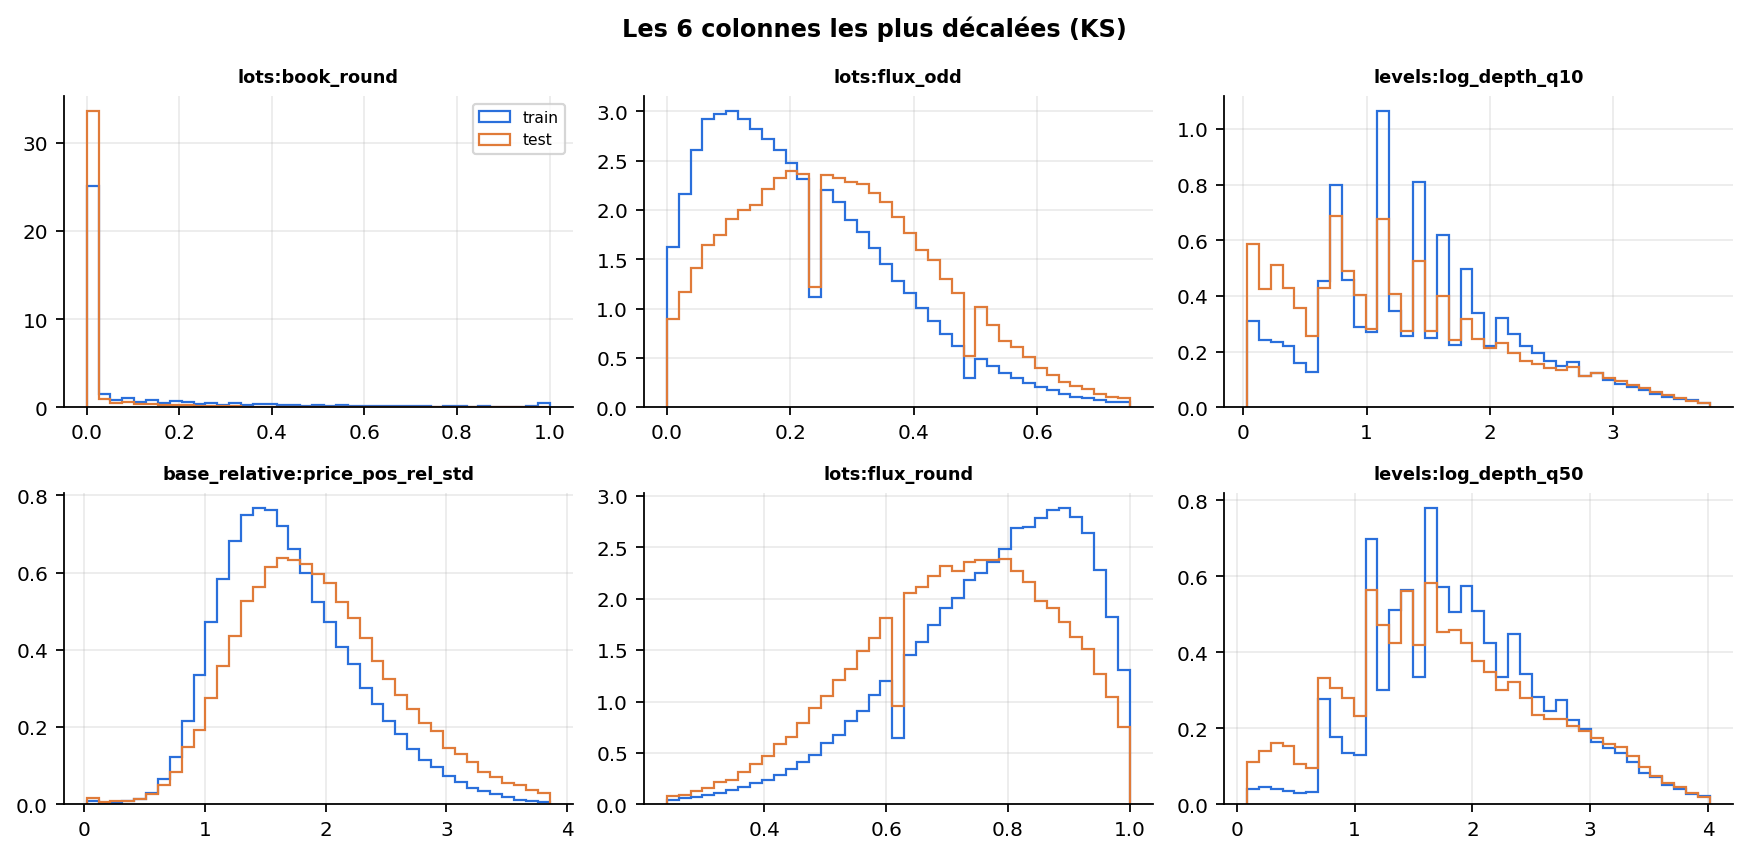
\includegraphics[width=\linewidth]{figures/demo_d3_top_shifts.png}
\caption{Les six colonnes les plus décalées entre train (bleu) et test (orange), au sens du test de Kolmogorov--Smirnov. Toutes appartiennent aux familles \emph{lots} et \emph{profondeur} : moins de lots ronds, plus d'odd lots, des carnets moins profonds. Aucune colonne de tick n'y figure.}
\end{figure}

\begin{figure}[H]\centering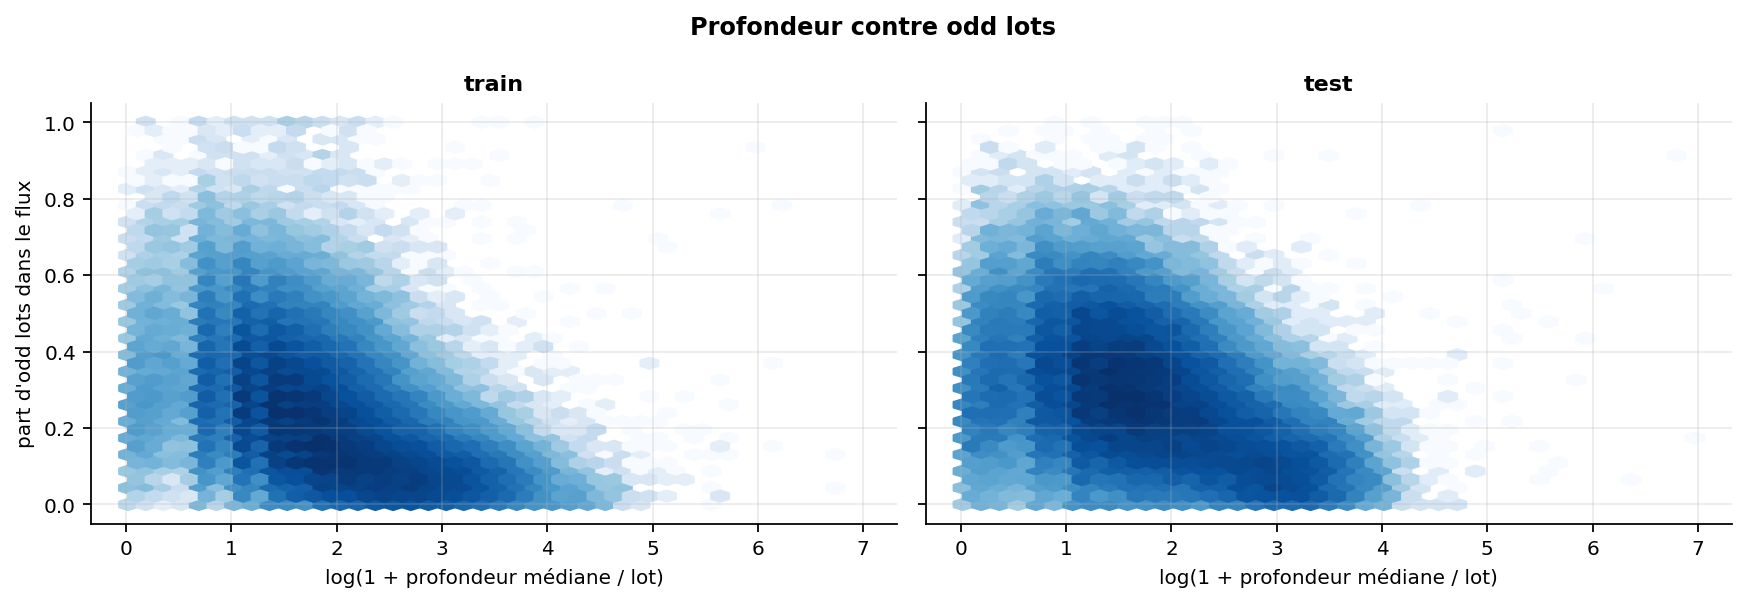
\includegraphics[width=.85\linewidth]{figures/demo_d3_depth_vs_oddlots.png}
\caption{Part d'odd lots en fonction de la profondeur, train contre test. La relation est décroissante dans les deux périodes, et le nuage du test glisse vers les carnets moins profonds et plus riches en odd lots. Un même mécanisme, des prix plus élevés, expliquerait les deux décalages à la fois : à valeur égale, moins d'actions par ordre.}
\end{figure}

\subsection{La vie des ordres}
\begin{figure}[H]\centering
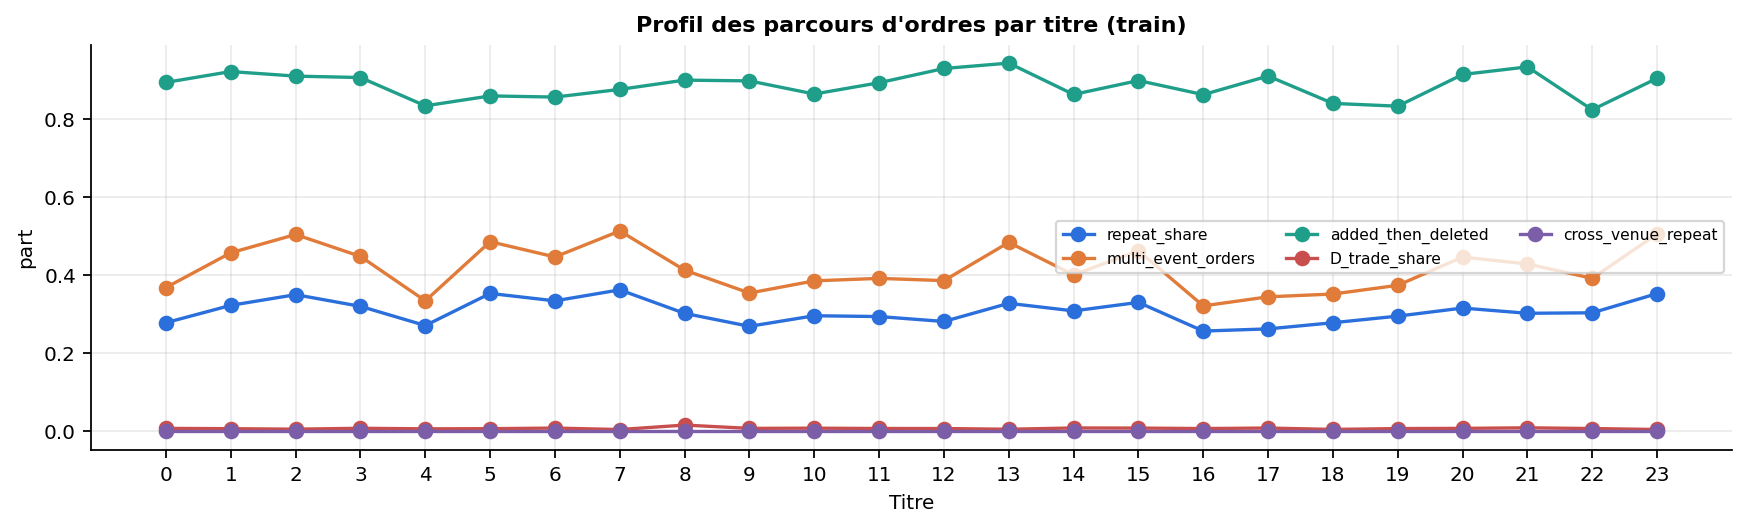
\includegraphics[width=.49\linewidth]{figures/demo_d4_profiles.png}\hfill
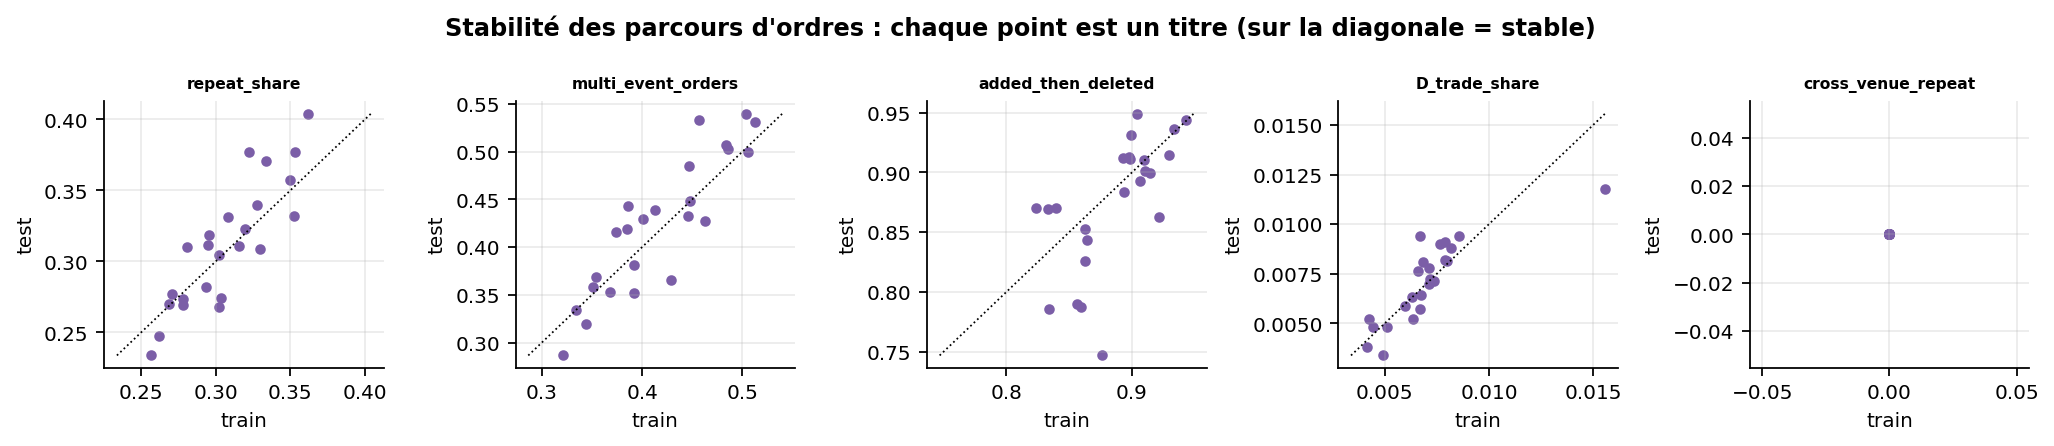
\includegraphics[width=.49\linewidth]{figures/demo_d4_train_vs_test.png}
\caption{À gauche, des profils de parcours d'ordres par titre : part d'ordres ajoutés puis supprimés dans la fenêtre (83 à 94\,\%), part d'ordres à plusieurs événements (33 à 50\,\%), part de répétitions. Les ordres exécutés sont rares. À droite, chaque point est un titre, train en abscisse et test en ordonnée. Les points restent proches de la diagonale : contrairement à la profondeur, la façon dont les ordres vivent et meurent est stable d'une période à l'autre.}
\end{figure}

\section{Unités naturelles : ticks et lots}\label{sec:unites}

\subsection{Les grandeurs de base}
Soit $\tick$ le tick estimé ($\tick=0{,}01$ sur le challenge) et $\lot$ la taille de lot ($\lot=100$, valeur de configuration). On définit, pour chaque événement $t$ d'une fenêtre (fichier \code{features/common.py}) :
\begin{align}
\text{cotation valide}\quad & \mathcal{Q}_t=\ind{b_t,\alpha_t\ \text{finis},\ \alpha_t\ge b_t},\\
\text{spread en ticks}\quad & S_t=\frac{\alpha_t-b_t}{\tick}\in\N\quad(\text{NaN si }\neg\mathcal{Q}_t),\\
\text{mid}\quad & m_t=\tfrac12(b_t+\alpha_t),\\
\text{variation du mid en demi-ticks}\quad & h_t=\frac{2(m_t-m_{t-1})}{\tick}\in\Z,\qquad h_1=0,\\
\text{distance au meilleur prix de son côté}\quad & D_t=\frac1\tick\begin{cases}b_t-p_t&\text{si }s_t=B,\\ p_t-\alpha_t&\text{si }s_t=A,\end{cases}\\
\text{tailles valides}\quad & \mathcal{V}_t=\ind{q^b_t,q^a_t\ \text{finis},\ \ge0},\\
\text{profondeur}\quad & Q_t=q^b_t+q^a_t\quad(\text{NaN si }\neg\mathcal{V}_t),\\
\text{imbalance}\quad & I_t=\frac{q^b_t-q^a_t}{Q_t}\in[-1,1]\quad(\text{NaN si }Q_t=0),\\
\text{flux en lots}\quad & F_t=f_t/\lot .
\end{align}
$D_t=0$ signifie « au meilleur prix » ; $D_t>0$, « plus profond dans le carnet » ; $D_t<0$, « dans le spread », c'est-à-dire un ordre qui améliore la cote. Un ordre d'achat placé à $b_t-2\tick$ et un ordre de vente placé à $\alpha_t+2\tick$ reçoivent tous deux $D_t=2$ : la grandeur est symétrique entre côtés par construction.

\begin{remarque}[Pourquoi des demi-ticks]
$m_t$ est la moyenne de deux multiples de $\tick$ : c'est un multiple de $\tick/2$. Donc $h_t$ est un entier. Un mid qui monte d'un demi-tick correspond exactement à une seule cotation (bid ou ask) qui monte d'un tick.
\end{remarque}

\subsection{Ce que la normalisation par médiane locale efface}
Le pipeline précédent utilisait des grandeurs relatives à la fenêtre, comme $r_t=S_t/s^\star$ avec $s^\star=\Med\{S_u:S_u>0\}$.

\begin{proposition}[Invariance d'échelle, donc perte d'échelle]\label{prop:scale}
Soit $g$ une fonction quelconque de la suite $(r_t)_t$. Pour tout $c>0$, remplacer $(S_t)$ par $(cS_t)$ laisse $g$ inchangée.
\end{proposition}
\begin{proof}
$s^\star(cS)=c\,s^\star(S)$, donc $r_t(cS)=cS_t/(c\,s^\star)=r_t(S)$.
\end{proof}
\begin{corollaire}
Une fenêtre au spread constant de 1 tick et une fenêtre au spread constant de 5 ticks ont exactement la même représentation relative ($r_t\equiv1$). Aucun modèle construit sur $r$ seul ne peut les distinguer.
\end{corollaire}
\noindent Or c'est précisément ce qui distingue un titre à \emph{gros tick} d'un titre à \emph{petit tick}. Pour un titre à gros tick, le tick est grand devant la volatilité intra-journalière : son spread reste presque toujours à 1 tick, et son mid saute par demi-ticks. Pour un titre à petit tick, le spread fluctue sur plusieurs ticks. Le pipeline précédent gardait ce niveau dans une feature séparée ($\log$ du spread médian). Mais il perdait la \emph{forme} discrète de la distribution : la part exacte du temps à 1 tick, à 2 ticks, etc.

Les parts en ticks conservent cette information :
\begin{equation}
\pi_k(W)=\frac{\sum_t\ind{S_t=k}}{\sum_t\mathcal{Q}_t},\quad k\in\{0,1,2\},\qquad \pi_{3\text{--}4},\ \pi_{\ge5}.
\end{equation}
Empiriquement (section~\ref{sec:resultats}), $\pi_{\ge5}$ et $\pi_1$ ont un pouvoir séparateur $\eta^2=0{,}56$ et $0{,}50$, pour une dérive train/test de seulement $\mathrm{KS}=0{,}02$. C'est la meilleure combinaison utilité/stabilité du screening.

\subsection{Lots : la convention de taille}
Pour une quantité non nulle $a=|F_t|$, on distingue :
\begin{equation}
\text{odd lot}: a<1,\qquad \text{lot rond}: a\in\{1,2,\dots\},\qquad \text{mixte}: a>1,\ a\notin\N .
\end{equation}
Les parts de chaque catégorie par fenêtre forment le bloc \code{lots}. Le pipeline précédent divisait le flux par sa médiane absolue $f^\star$. Or $f^\star$ vaut presque toujours exactement $\lot$ : sur la figure 04 du pipeline précédent, $\log(1+f^\star)$ est concentré à $\log 101\approx4{,}62$. Cette normalisation revenait donc à diviser par $\lot$, sans exprimer ce qui distingue vraiment les titres : la \emph{fréquence} des odd lots et des tailles mixtes.

\subsection{Une redondance évitée : le microprice}
\begin{lemme}
Soit le microprice $\mu_t=\dfrac{\alpha_tq^b_t+b_tq^a_t}{q^b_t+q^a_t}$. Alors $\dfrac{\mu_t-m_t}{\alpha_t-b_t}=\dfrac{I_t}{2}$.
\end{lemme}
\begin{proof}
$\mu_t-m_t=\dfrac{\alpha_tq^b+b_tq^a}{Q}-\dfrac{(\alpha_t+b_t)(q^b+q^a)}{2Q}=\dfrac{(\alpha_t-b_t)(q^b-q^a)}{2Q}$.
\end{proof}
\noindent Ajouter le microprice normalisé en plus de l'imbalance n'apporterait qu'une copie linéaire.

\subsection{Données invalides}
Une cotation croisée ($\alpha_t<b_t$), une taille négative ou une valeur non finie produisent des NaN dans les grandeurs dérivées. Elles ne produisent jamais un 0, qui serait une fausse valeur plausible. Les statistiques de fenêtre sont calculées sur les valeurs finies seulement :
\begin{equation}
\overline{x}(W)=\frac{\sum_t x_t\ind{x_t\ \text{fini}}}{\sum_t\ind{x_t\ \text{fini}}},
\end{equation}
et valent NaN si aucune valeur n'est finie. Les arbres gèrent nativement les NaN. Les réseaux les remplacent par la moyenne du fit (soit 0 après standardisation). La part de tailles nulles à une cotation valide et la part de tailles négatives sont elles-mêmes des features (bloc \code{lots}). Cette question avait été soulevée sur la figure 01 du pipeline précédent, avec un \code{ask\_size} nul pendant 48 événements.

\section{Parcours d'ordres et tokens d'événements}\label{sec:ordres}

\subsection{Parcours d'un ordre dans une fenêtre tronquée}
Pour l'événement $t$, notons $\mathcal{P}(t)=\{u<t:\rho(u)=\rho(t)\}$ les occurrences \emph{antérieures} du même ordre dans la fenêtre. On définit :
\begin{align}
\text{occurrence}\quad & n_t=|\mathcal{P}(t)|\qquad(0=\text{première fois vu}),\\
\text{occurrence précédente}\quad & \operatorname{prev}(t)=\max\mathcal{P}(t)\quad(\text{indéfini si }n_t=0),\\
\text{écart}\quad & g_t=t-\operatorname{prev}(t)\quad(0\text{ si }n_t=0),\\
\text{action précédente du même ordre}\quad & a^{\leftarrow}_t=a_{\operatorname{prev}(t)}\quad(0\text{ si }n_t=0),\\
\text{première action}\quad & a^{\circ}_t=a_{\min(\mathcal{P}(t)\cup\{t\})},\\
\text{nombre d'événements de l'ordre}\quad & N_t=|\{u\le L:\rho(u)=\rho(t)\}| .
\end{align}

\begin{remarque}[Troncature]
La fenêtre est un extrait. Une première apparition sous forme $U$ ou $D$ révèle un ordre créé \emph{avant} la fenêtre. Une première apparition $A$ est un ajout \emph{observé}. Aucune de ces grandeurs n'est une durée de vie, un volume initial ou une identité de participant. $g_t$ est compté en événements, pas en secondes : aucun horodatage n'est disponible.
\end{remarque}

\paragraph{Calcul exact et vectorisé.}
On numérote les événements d'un bloc de $m$ fenêtres à plat, $j=iL+t$, et on forme la clé $k_j=128\,i+\rho_{i,t}$, avec $\rho<100<128$. Un tri \emph{stable} $\sigma$ des clés regroupe les événements de chaque (fenêtre, ordre). Comme le tri est stable et que les positions plates sont croissantes dans le temps, les occurrences d'un même ordre restent dans l'ordre chronologique. Notons $\kappa=k_{\sigma(\cdot)}$ la suite triée et $\nu_r=\ind{r=0\ \text{ou}\ \kappa_r\neq\kappa_{r-1}}$ le début de groupe. Alors
\begin{align}
\text{début}(r)&=\max\{r'\le r:\nu_{r'}=1\},\\
n_{\sigma(r)}&=r-\text{début}(r),\\
\operatorname{prev}(\sigma(r))&=\begin{cases}\sigma(r-1)&\text{si }\nu_r=0,\\\text{indéfini}&\text{sinon,}\end{cases}\\
a^{\circ}_{\sigma(r)}&=a_{\sigma(\text{début}(r))}.
\end{align}
\begin{proposition}
Ces formules donnent exactement les définitions ci-dessus.
\end{proposition}
\begin{proof}
Dans un groupe (même fenêtre, même $\rho$), le tri stable conserve l'ordre croissant des positions plates, donc l'ordre chronologique. Le $r$-ième élément d'un groupe a donc $r-\text{début}(r)$ prédécesseurs dans ce groupe ; son prédécesseur immédiat est l'élément trié juste avant lui ; et le premier élément du groupe est la première apparition.
\end{proof}
\noindent Le test de contrat compare ces calculs à une boucle naïve sur des données aléatoires.

\subsection{Tokens : discrétiser sans rien apprendre}
\begin{definition}[Bucket à seuils fixés]
Pour des seuils $c_1<\dots<c_J$ \emph{choisis a priori}, on pose
\begin{equation}
B(x;c)=\begin{cases}0&x\ \text{non fini},\\1+\#\{j:c_j\le x\}&\text{sinon,}\end{cases}\qquad B\in\{0,\dots,J+1\}.
\end{equation}
\end{definition}

\begin{table}[H]\centering\small
\begin{tabular}{llcl}
\toprule
Token & Grandeur & Card. & Valeurs\\
\midrule
\code{tok\_action} & $a_t$ & 4 & inconnu, A, D, U\\
\code{tok\_side} & $s_t$ & 3 & inconnu, A, B\\
\code{tok\_trade} & $\tau_t$ & 3 & inconnu, non, oui\\
\code{tok\_venue} & $v_t$ & 16 & inconnue, 6 places (réservé jusqu'à 15)\\
\code{tok\_pos} & $B(D_t;-.5,.5,1.5,2.5,5.5)$ & 7 & ?, dans le spread, au meilleur, 1, 2, 3--5, $>5$ ticks\\
\code{tok\_size} & $B(|F_t|;10^{-9},1^{\pm},2^+,5^+,10^+)$ & 8 & ?, 0, odd, $=1$ lot, $(1,2]$, $(2,5]$, $(5,10]$, $>10$\\
\code{tok\_spread} & $B(S_t;.5,1.5,2.5,4.5)$ & 6 & ?, 0, 1, 2, 3--4, $\ge5$ ticks\\
\code{tok\_dmid} & $B(h_t;-1.5,-.25,.25,1.5)$ & 6 & ?, $\le-1{,}5$, baisse, 0, hausse, $\ge1{,}5$ demi-tick\\
\code{tok\_occ} & $1+\min(n_t,3)$ & 5 & 1\textsuperscript{re}, 2\textsuperscript{e}, 3\textsuperscript{e}, 4\textsuperscript{e}+ occurrence\\
\code{tok\_prev\_action} & $a^{\leftarrow}_t$ & 4 & aucune, A, D, U\\
\code{tok\_fluxsign} & $B(f_t;-10^{-12},10^{-12})$ & 4 & ?, $<0$, $0$, $>0$\\
\bottomrule
\end{tabular}
\caption{Les onze tokens. $1^{\pm}$ désigne les deux seuils $1\mp10^{-9}$ qui isolent « exactement un lot ».}
\end{table}

\begin{proposition}[Absence de fuite par construction]
L'application $e_t\mapsto(\text{tokens})$ est une fonction déterministe de l'événement, de sa fenêtre et des constantes $(\tick,\lot)$. Elle ne dépend d'aucune autre fenêtre ni d'aucun label. En particulier, elle est identique au développement, au refit et sur le test.
\end{proposition}
\noindent Le seul paramètre « appris » en amont est $\hat\tick$. Il est estimé sur les prix du train, sans labels, et il est vérifié égal à la grille ($0{,}01$).

\paragraph{Taille du vocabulaire.} Le produit cartésien des cardinalités vaut
\begin{equation}
4\cdot3\cdot3\cdot16\cdot7\cdot8\cdot6\cdot6\cdot5\cdot4\cdot4= 92\,897\,280\approx 9{,}3\cdot10^{7},
\end{equation}
mais un événement n'est pas représenté par un mot de ce produit. Il est représenté par la \emph{somme} de 11 embeddings (section~\ref{sec:embed}), qui ne coûte que $\sum_j\text{card}_j=66$ vecteurs. Les interactions entre tokens (« une suppression, côté ask, au meilleur ») sont apprises par les couches suivantes.

\subsection{Canaux continus par événement}
En complément des tokens, chaque événement porte des canaux réels :
\begin{align}
\code{ev\_relative}&:\ \big(I_t,\ \log(1+Q_t/d^\star),\ \operatorname{asinh}(\Delta Q_t/d^\star),\ \operatorname{slog}(f_t/f^\star),\ \log(1+g_t)\big),\\
\code{ev\_levels}&:\ \big(\log(1+q^b_t/\lot),\ \log(1+q^a_t/\lot),\ \operatorname{slog}F_t,\ \log(1+S_t),\ \operatorname{asinh}D_t,\ \operatorname{asinh}h_t\big),
\end{align}
avec $\operatorname{slog}(x)=\operatorname{sign}(x)\log(1+|x|)$, et $d^\star$, $f^\star$ les médianes positives de la fenêtre (repli à 1). La version 0.2.0 sépare \code{ev\_levels} en \code{ev\_ticks} (les trois derniers canaux) et \code{ev\_sizes} (les trois premiers), pour pouvoir retirer les tailles absolues sans retirer les ticks.

\section{Un exemple complet : de la fenêtre brute aux tokens}\label{sec:exemple}

Les définitions des sections~\ref{sec:unites} et~\ref{sec:ordres} sont plus faciles à saisir sur un cas réel. Nous construisons à la main un motif de 20 événements qui passe par les situations intéressantes :
\begin{itemize}
\item un ordre déjà présent avant la fenêtre ;
\item des ajouts au meilleur prix et plus profond ;
\item des exécutions, dont une qui vide le meilleur niveau ;
\item un odd lot, une taille mixte ;
\item une amélioration de la cote, puis une annulation immédiate ;
\item un même ordre qui change de venue ;
\item un gros ordre lointain.
\end{itemize}
La fenêtre passée au code répète ce motif cinq fois (100 événements, avec des identifiants renouvelés à chaque répétition).

\textbf{Tous les nombres de cette section sont produits par le code du pipeline} (\code{cfm.features}), via le script \code{paper/examples/make\_examples.py}. Ils ne sont pas recopiés à la main.

\subsection{Étape 0 : les événements bruts}
Prix recentrés sur le premier bid, $\tick=0{,}01$ et $\lot=100$ : c'est exactement ce que contient le CSV du challenge.

\begin{table}[H]\centering\scriptsize
\begin{tabular}{rrrcccrrrrcrl}
\toprule
$t$ & venue & order\_id & act. & côté & price & bid & ask & $q^b$ & $q^a$ & trade & flux\\
\midrule
1 & 0 & 5012 & U & B & 0 & 0 & 0{,}01 & 300 & 200 & non & $-$100\\
2 & 1 & 7731 & A & A & 0{,}01 & 0 & 0{,}01 & 300 & 300 & non & 100\\
3 & 1 & 2210 & A & B & $-$0{,}02 & 0 & 0{,}01 & 300 & 300 & non & 200\\
4 & 0 & 7731 & D & A & 0{,}01 & 0 & 0{,}01 & 300 & 200 & oui & $-$100\\
5 & 2 & 9002 & A & A & 0{,}02 & 0 & 0{,}01 & 300 & 200 & non & 37\\
6 & 0 & 5012 & D & B & 0 & 0 & 0{,}01 & 100 & 200 & non & $-$200\\
7 & 3 & 1180 & D & A & 0{,}01 & 0 & 0{,}02 & 100 & 37 & oui & $-$200\\
8 & 1 & 2210 & U & B & $-$0{,}02 & 0 & 0{,}02 & 100 & 37 & non & 100\\
9 & 2 & 4040 & A & A & 0{,}01 & 0 & 0{,}01 & 100 & 100 & non & 100\\
10 & 2 & 4040 & D & A & 0{,}01 & 0 & 0{,}02 & 100 & 37 & non & $-$100\\
11 & 0 & 3333 & A & B & 0{,}01 & 0{,}01 & 0{,}02 & 150 & 37 & non & 150\\
12 & 4 & 9002 & U & A & 0{,}02 & 0{,}01 & 0{,}02 & 150 & 100 & non & 63\\
13 & 4 & 3333 & D & B & 0{,}01 & 0 & 0{,}02 & 100 & 100 & oui & $-$150\\
14 & 5 & 8888 & A & B & $-$0{,}06 & 0 & 0{,}02 & 100 & 100 & non & 1000\\
15 & 5 & 8888 & U & B & $-$0{,}06 & 0 & 0{,}02 & 100 & 100 & non & $-$500\\
16 & 0 & 1212 & A & A & 0{,}02 & 0 & 0{,}02 & 100 & 200 & non & 100\\
17 & 0 & 1212 & U & A & 0{,}02 & 0 & 0{,}02 & 100 & 300 & non & 100\\
18 & 3 & 1212 & D & A & 0{,}02 & 0 & 0{,}03 & 100 & 400 & oui & $-$300\\
19 & 1 & 7070 & A & A & 0{,}02 & 0 & 0{,}02 & 100 & 100 & non & 100\\
20 & 1 & 2210 & D & B & $-$0{,}02 & 0 & 0{,}02 & 100 & 100 & non & $-$300\\
\bottomrule
\end{tabular}
\caption{Le motif brut. B = côté acheteur (bid), A = côté vendeur (ask). Les colonnes bid, ask, $q^b$ et $q^a$ décrivent le carnet agrégé \emph{après} l'événement.}
\label{tab:exraw}
\end{table}

\begin{figure}[H]\centering
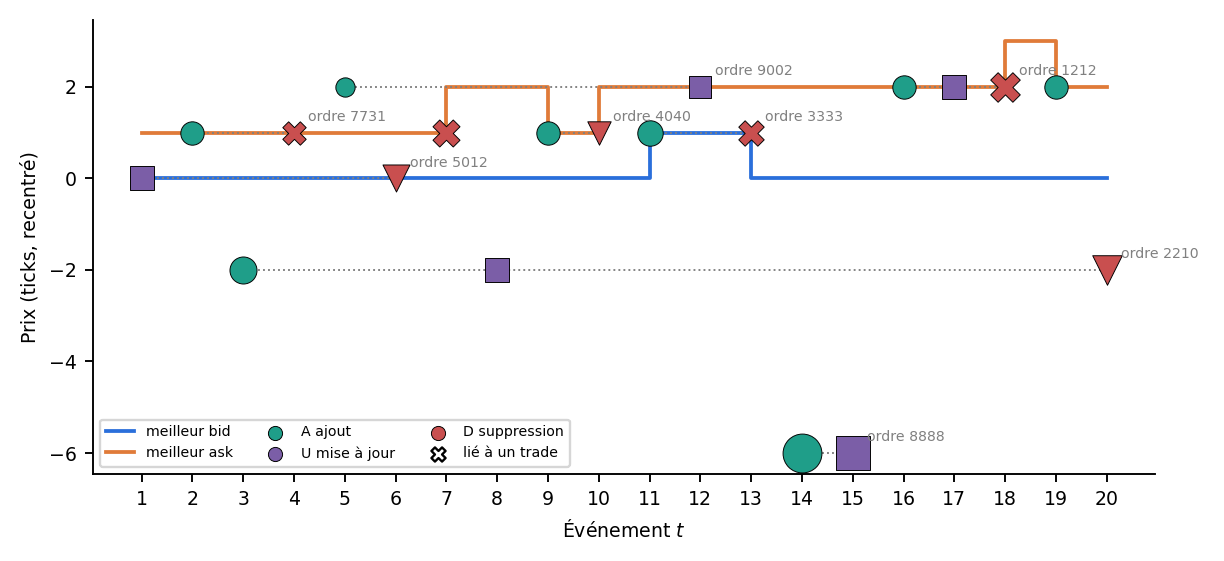
\includegraphics[width=\linewidth]{figures/ex_motif.png}
\caption{Le motif en image. Les escaliers sont les meilleures limites ; chaque marqueur est un événement (couleur = action, croix = lié à un trade, taille $\propto\sqrt{|f|}$). Les pointillés relient les événements d'un \emph{même ordre} : ce sont les parcours que les tokens d'occurrence et d'action précédente encodent.}
\label{fig:exmotif}
\end{figure}

\subsection{Étape 1 : l'identité des ordres}
Les identifiants bruts (5012, 7731, \dots) sont remplacés par leur rang de première apparition $\rho_t$ (section~\ref{sec:donnees}). Seules les égalités comptent : 5012 devient 0, 7731 devient 1, 2210 devient 2, etc. On en déduit l'occurrence $n_t$, l'action précédente du même ordre $a^{\leftarrow}_t$ et l'écart $g_t$ (tableau~\ref{tab:exderived}). Trois parcours se lisent directement :

\begin{itemize}
\item \textbf{L'ordre 2210} ($\rho=2$) apparaît à $t=3$ (ajout), $t=8$ (mise à jour) et $t=20$ (suppression). On obtient $n=(0,1,2)$, $a^{\leftarrow}=(\text{—},A,U)$ et $g=(0,5,12)$.
\item \textbf{L'ordre 5012} ($\rho=0$) apparaît d'abord sous forme d'une \emph{mise à jour}. Il existait donc avant la fenêtre : la troncature est visible. Dans le bloc \code{orders}, il compte dans \code{first\_seen\_U}.
\item \textbf{L'ordre 1212} ($\rho=8$) est ajouté puis modifié sur la venue 0, puis exécuté sur la venue 3 ($t=18$). C'est une répétition « inter-venue », possible parce que le carnet est agrégé (\code{cross\_venue\_repeat}).
\end{itemize}

\subsection{Étape 2 : passer en unités naturelles}
\begin{table}[H]\centering\scriptsize
\begin{tabular}{rrrrrrrrrl}
\toprule
$t$ & $\rho_t$ & $n_t$ & $a^{\leftarrow}_t$ & $g_t$ & $S_t$ & $h_t$ & $D_t$ & $F_t$ & lecture\\
\midrule
1 & 0 & 0 & — & 0 & 1 & 0 & 0 & $-$1 & \parbox[t]{6.2cm}{\raggedright\scriptsize ordre déjà présent avant la fenêtre (1re apparition = U), réduit d'un lot}\\
2 & 1 & 0 & — & 0 & 1 & 0 & 0 & 1 & \parbox[t]{6.2cm}{\raggedright\scriptsize ajout d'un lot au meilleur ask}\\
3 & 2 & 0 & — & 0 & 1 & 0 & 2 & 2 & \parbox[t]{6.2cm}{\raggedright\scriptsize ajout de 2 lots, 2 ticks derrière le meilleur bid}\\
4 & 1 & 1 & A & 2 & 1 & 0 & 0 & $-$1 & \parbox[t]{6.2cm}{\raggedright\scriptsize l'ordre de t=2 est exécuté (suppression liée à un trade)}\\
5 & 3 & 0 & — & 0 & 1 & 0 & 1 & 0{,}37 & \parbox[t]{6.2cm}{\raggedright\scriptsize odd lot (37 actions), 1 tick derrière le meilleur ask}\\
6 & 0 & 1 & U & 5 & 1 & 0 & 0 & $-$2 & \parbox[t]{6.2cm}{\raggedright\scriptsize annulation de l'ordre pré-existant}\\
7 & 4 & 0 & — & 0 & 2 & 1 & $-$1 & $-$2 & \parbox[t]{6.2cm}{\raggedright\scriptsize trade vide le meilleur ask : l'ask passe à 0,02, spread 2 ticks, le mid monte d'un demi-tick}\\
8 & 2 & 1 & A & 5 & 2 & 0 & 2 & 1 & \parbox[t]{6.2cm}{\raggedright\scriptsize l'ordre profond de t=3 grossit d'un lot}\\
9 & 5 & 0 & — & 0 & 1 & $-$1 & 0 & 1 & \parbox[t]{6.2cm}{\raggedright\scriptsize ajout DANS le spread : améliore l'ask}\\
10 & 5 & 1 & A & 1 & 2 & 1 & $-$1 & $-$1 & \parbox[t]{6.2cm}{\raggedright\scriptsize le même ordre est annulé aussitôt (ajouté puis supprimé)}\\
11 & 6 & 0 & — & 0 & 1 & 1 & 0 & 1{,}5 & \parbox[t]{6.2cm}{\raggedright\scriptsize ajout DANS le spread côté bid, taille mixte (1,5 lot)}\\
12 & 3 & 1 & A & 7 & 1 & 0 & 0 & 0{,}63 & \parbox[t]{6.2cm}{\raggedright\scriptsize l'odd lot de t=5 est complété à un lot rond}\\
13 & 6 & 1 & A & 2 & 2 & $-$1 & $-$1 & $-$1{,}5 & \parbox[t]{6.2cm}{\raggedright\scriptsize l'ordre de t=11 est exécuté : le bid redescend}\\
14 & 7 & 0 & — & 0 & 2 & 0 & 6 & 10 & \parbox[t]{6.2cm}{\raggedright\scriptsize gros ordre (10 lots) très loin (6 ticks)}\\
15 & 7 & 1 & A & 1 & 2 & 0 & 6 & $-$5 & \parbox[t]{6.2cm}{\raggedright\scriptsize réduit de moitié}\\
16 & 8 & 0 & — & 0 & 2 & 0 & 0 & 1 & \parbox[t]{6.2cm}{\raggedright\scriptsize ajout d'un lot au meilleur ask}\\
17 & 8 & 1 & A & 1 & 2 & 0 & 0 & 1 & \parbox[t]{6.2cm}{\raggedright\scriptsize le même ordre grossit}\\
18 & 8 & 2 & U & 1 & 3 & 1 & $-$1 & $-$3 & \parbox[t]{6.2cm}{\raggedright\scriptsize exécuté sur une AUTRE venue (3) : l'ask passe à 0,03, spread 3 ticks}\\
19 & 9 & 0 & — & 0 & 2 & $-$1 & 0 & 1 & \parbox[t]{6.2cm}{\raggedright\scriptsize ajout dans le spread, l'ask revient à 0,02}\\
20 & 2 & 2 & U & 12 & 2 & 0 & 2 & $-$3 & \parbox[t]{6.2cm}{\raggedright\scriptsize annulation de l'ordre profond de t=3}\\
\bottomrule
\end{tabular}
\caption{Grandeurs dérivées, calculées par \code{features/common.py} : spread $S_t$ en ticks, variation du mid $h_t$ en demi-ticks, distance au meilleur prix de son côté $D_t$ en ticks, flux $F_t$ en lots.}
\label{tab:exderived}
\end{table}

\paragraph{Quatre calculs détaillés.}
\begin{itemize}
\item \textbf{$t=5$} (odd lot, côté ask, prix $0{,}02$, ask après l'événement $0{,}01$) :
$D_5=(p_5-\alpha_5)/\tick=(0{,}02-0{,}01)/0{,}01=1$, soit un tick derrière le meilleur ask ; $F_5=37/100=0{,}37<1$, donc un odd lot.
\item \textbf{$t=7$} (un trade vide le meilleur ask) : l'ask passe de $0{,}01$ à $0{,}02$, donc $S_7=2$. Le mid passe de $0{,}005$ à $0{,}010$, donc $h_7=2\times0{,}005/0{,}01=1$ : une hausse d'un demi-tick.
\item \textbf{$t=11$} (ajout côté bid à $0{,}01$, qui améliore le bid) : après l'événement, $b_{11}=0{,}01$, donc $D_{11}=(b_{11}-p_{11})/\tick=0$, et $F_{11}=1{,}5$, une taille mixte.
\item \textbf{$t=14$} (gros ordre lointain) : $D_{14}=(0-(-0{,}06))/0{,}01=6$ et $F_{14}=10$ lots.
\end{itemize}

\subsection{Étape 3 : discrétiser en tokens}
Chaque grandeur passe par une fonction de bucket à seuils fixés, $B(x;c)=1+\#\{j:c_j\le x\}$ (0 si $x$ n'est pas défini).

Pour la taille, les seuils sont $c=(10^{-9},\,1-10^{-9},\,1+10^{-9},\,2+10^{-9},\,5+10^{-9},\,10+10^{-9})$ :
\begin{align*}
t=5:&\quad B(0{,}37;c)=1+\#\{10^{-9}\}=2\ \Rightarrow\ \text{« odd »},\\
t=1:&\quad B(1;c)=1+\#\{10^{-9},\,1-10^{-9}\}=3\ \Rightarrow\ \text{« = 1 lot »},\\
t=14:&\quad B(10;c)=1+5=6\ \Rightarrow\ \text{« (5,10] »}.
\end{align*}
Les deux seuils $1\pm10^{-9}$ isolent exactement « un lot rond », qui est la taille la plus fréquente sur ce marché.

\begin{table}[H]\centering\scriptsize\setlength{\tabcolsep}{2.5pt}
\begin{tabular}{rccccccccccc}
\toprule
$t$ & act & côté & trade & venue & pos & taille & spread & Δmid & occ & préc. & signe\\
\midrule
1 & 3\,{\tiny(U)} & 2\,{\tiny(bid)} & 1\,{\tiny(non)} & 1\,{\tiny(v0)} & 2\,{\tiny(=)} & 3\,{\tiny(=1 lot)} & 2\,{\tiny(1)} & 3\,{\tiny(0)} & 1\,{\tiny(1re)} & 0\,{\tiny(aucune)} & 1\,{\tiny(<0)}\\
2 & 1\,{\tiny(A)} & 1\,{\tiny(ask)} & 1\,{\tiny(non)} & 2\,{\tiny(v1)} & 2\,{\tiny(=)} & 3\,{\tiny(=1 lot)} & 2\,{\tiny(1)} & 3\,{\tiny(0)} & 1\,{\tiny(1re)} & 0\,{\tiny(aucune)} & 3\,{\tiny(>0)}\\
3 & 1\,{\tiny(A)} & 2\,{\tiny(bid)} & 1\,{\tiny(non)} & 2\,{\tiny(v1)} & 4\,{\tiny(+2)} & 4\,{\tiny((1,2])} & 2\,{\tiny(1)} & 3\,{\tiny(0)} & 1\,{\tiny(1re)} & 0\,{\tiny(aucune)} & 3\,{\tiny(>0)}\\
4 & 2\,{\tiny(D)} & 1\,{\tiny(ask)} & 2\,{\tiny(oui)} & 1\,{\tiny(v0)} & 2\,{\tiny(=)} & 3\,{\tiny(=1 lot)} & 2\,{\tiny(1)} & 3\,{\tiny(0)} & 2\,{\tiny(2e)} & 1\,{\tiny(A)} & 1\,{\tiny(<0)}\\
5 & 1\,{\tiny(A)} & 1\,{\tiny(ask)} & 1\,{\tiny(non)} & 3\,{\tiny(v2)} & 3\,{\tiny(+1)} & 2\,{\tiny(odd)} & 2\,{\tiny(1)} & 3\,{\tiny(0)} & 1\,{\tiny(1re)} & 0\,{\tiny(aucune)} & 3\,{\tiny(>0)}\\
6 & 2\,{\tiny(D)} & 2\,{\tiny(bid)} & 1\,{\tiny(non)} & 1\,{\tiny(v0)} & 2\,{\tiny(=)} & 4\,{\tiny((1,2])} & 2\,{\tiny(1)} & 3\,{\tiny(0)} & 2\,{\tiny(2e)} & 3\,{\tiny(U)} & 1\,{\tiny(<0)}\\
7 & 2\,{\tiny(D)} & 1\,{\tiny(ask)} & 2\,{\tiny(oui)} & 4\,{\tiny(v3)} & 1\,{\tiny(in)} & 4\,{\tiny((1,2])} & 3\,{\tiny(2)} & 4\,{\tiny(hausse)} & 1\,{\tiny(1re)} & 0\,{\tiny(aucune)} & 1\,{\tiny(<0)}\\
8 & 3\,{\tiny(U)} & 2\,{\tiny(bid)} & 1\,{\tiny(non)} & 2\,{\tiny(v1)} & 4\,{\tiny(+2)} & 3\,{\tiny(=1 lot)} & 3\,{\tiny(2)} & 3\,{\tiny(0)} & 2\,{\tiny(2e)} & 1\,{\tiny(A)} & 3\,{\tiny(>0)}\\
9 & 1\,{\tiny(A)} & 1\,{\tiny(ask)} & 1\,{\tiny(non)} & 3\,{\tiny(v2)} & 2\,{\tiny(=)} & 3\,{\tiny(=1 lot)} & 2\,{\tiny(1)} & 2\,{\tiny(baisse)} & 1\,{\tiny(1re)} & 0\,{\tiny(aucune)} & 3\,{\tiny(>0)}\\
10 & 2\,{\tiny(D)} & 1\,{\tiny(ask)} & 1\,{\tiny(non)} & 3\,{\tiny(v2)} & 1\,{\tiny(in)} & 3\,{\tiny(=1 lot)} & 3\,{\tiny(2)} & 4\,{\tiny(hausse)} & 2\,{\tiny(2e)} & 1\,{\tiny(A)} & 1\,{\tiny(<0)}\\
11 & 1\,{\tiny(A)} & 2\,{\tiny(bid)} & 1\,{\tiny(non)} & 1\,{\tiny(v0)} & 2\,{\tiny(=)} & 4\,{\tiny((1,2])} & 2\,{\tiny(1)} & 4\,{\tiny(hausse)} & 1\,{\tiny(1re)} & 0\,{\tiny(aucune)} & 3\,{\tiny(>0)}\\
12 & 3\,{\tiny(U)} & 1\,{\tiny(ask)} & 1\,{\tiny(non)} & 5\,{\tiny(v4)} & 2\,{\tiny(=)} & 2\,{\tiny(odd)} & 2\,{\tiny(1)} & 3\,{\tiny(0)} & 2\,{\tiny(2e)} & 1\,{\tiny(A)} & 3\,{\tiny(>0)}\\
13 & 2\,{\tiny(D)} & 2\,{\tiny(bid)} & 2\,{\tiny(oui)} & 5\,{\tiny(v4)} & 1\,{\tiny(in)} & 4\,{\tiny((1,2])} & 3\,{\tiny(2)} & 2\,{\tiny(baisse)} & 2\,{\tiny(2e)} & 1\,{\tiny(A)} & 1\,{\tiny(<0)}\\
14 & 1\,{\tiny(A)} & 2\,{\tiny(bid)} & 1\,{\tiny(non)} & 6\,{\tiny(v5)} & 6\,{\tiny(>+5)} & 6\,{\tiny((5,10])} & 3\,{\tiny(2)} & 3\,{\tiny(0)} & 1\,{\tiny(1re)} & 0\,{\tiny(aucune)} & 3\,{\tiny(>0)}\\
15 & 3\,{\tiny(U)} & 2\,{\tiny(bid)} & 1\,{\tiny(non)} & 6\,{\tiny(v5)} & 6\,{\tiny(>+5)} & 5\,{\tiny((2,5])} & 3\,{\tiny(2)} & 3\,{\tiny(0)} & 2\,{\tiny(2e)} & 1\,{\tiny(A)} & 1\,{\tiny(<0)}\\
16 & 1\,{\tiny(A)} & 1\,{\tiny(ask)} & 1\,{\tiny(non)} & 1\,{\tiny(v0)} & 2\,{\tiny(=)} & 3\,{\tiny(=1 lot)} & 3\,{\tiny(2)} & 3\,{\tiny(0)} & 1\,{\tiny(1re)} & 0\,{\tiny(aucune)} & 3\,{\tiny(>0)}\\
17 & 3\,{\tiny(U)} & 1\,{\tiny(ask)} & 1\,{\tiny(non)} & 1\,{\tiny(v0)} & 2\,{\tiny(=)} & 3\,{\tiny(=1 lot)} & 3\,{\tiny(2)} & 3\,{\tiny(0)} & 2\,{\tiny(2e)} & 1\,{\tiny(A)} & 3\,{\tiny(>0)}\\
18 & 2\,{\tiny(D)} & 1\,{\tiny(ask)} & 2\,{\tiny(oui)} & 4\,{\tiny(v3)} & 1\,{\tiny(in)} & 5\,{\tiny((2,5])} & 4\,{\tiny(3–4)} & 4\,{\tiny(hausse)} & 3\,{\tiny(3e)} & 3\,{\tiny(U)} & 1\,{\tiny(<0)}\\
19 & 1\,{\tiny(A)} & 1\,{\tiny(ask)} & 1\,{\tiny(non)} & 2\,{\tiny(v1)} & 2\,{\tiny(=)} & 3\,{\tiny(=1 lot)} & 3\,{\tiny(2)} & 2\,{\tiny(baisse)} & 1\,{\tiny(1re)} & 0\,{\tiny(aucune)} & 3\,{\tiny(>0)}\\
20 & 2\,{\tiny(D)} & 2\,{\tiny(bid)} & 1\,{\tiny(non)} & 2\,{\tiny(v1)} & 4\,{\tiny(+2)} & 5\,{\tiny((2,5])} & 3\,{\tiny(2)} & 3\,{\tiny(0)} & 3\,{\tiny(3e)} & 3\,{\tiny(U)} & 1\,{\tiny(<0)}\\
\bottomrule
\end{tabular}
\caption{Les onze tokens de chaque événement : l'indice d'abord, la signification entre parenthèses. Pour \code{pos}, « in » signifie « dans le spread », « = » « au meilleur » et « $+k$ » « $k$ ticks derrière ».}
\label{tab:extokens}
\end{table}

\begin{figure}[H]\centering
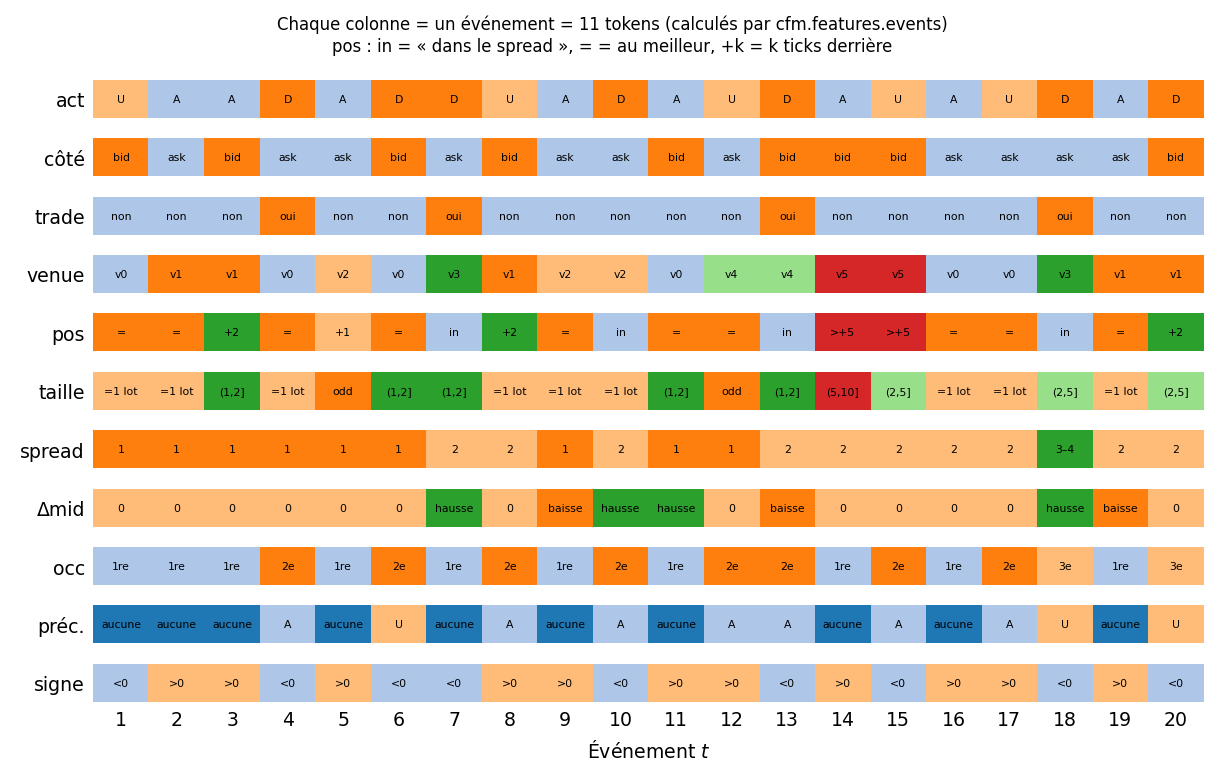
\includegraphics[width=\linewidth]{figures/ex_tokens.png}
\caption{La même information en bandeau : une colonne par événement, une ligne par token. C'est littéralement ce que voit SignatureNet avant ses couches d'embedding.}
\label{fig:extokens}
\end{figure}

\subsection{Ce que l'exemple révèle : $D_t$ est mesuré \emph{après} l'événement}\label{sec:dpost}
L'exemple met au jour une subtilité de la définition. Elle n'apparaît pas à la lecture des formules.

\begin{itemize}
\item \textbf{Ajouts qui améliorent la cote ($t=9$, $t=11$).} L'ordre devient lui-même le meilleur prix. Il est donc codé « = » (au meilleur), et non « in » (dans le spread).
\item \textbf{Suppressions qui vident le meilleur niveau ($t=7,10,13,18$).} Après l'événement, la meilleure limite a reculé, et le prix de l'ordre supprimé se retrouve \emph{à l'intérieur} du nouveau spread : $D_t=-1$, codé « in ».
\end{itemize}

Dans le pipeline actuel, le token « in » signifie donc en pratique « \emph{cet événement a vidé le meilleur niveau} ». C'est une information utile, que le modèle a exploitée telle quelle (LB $0{,}6351$), mais son nom est trompeur. La correction naturelle consiste à mesurer la position par rapport au carnet \emph{avant} l'événement :
\begin{equation}
D^{\text{pré}}_t=\frac1\tick\begin{cases}b_{t-1}-p_t&s_t=B,\\ p_t-\alpha_{t-1}&s_t=A.\end{cases}
\end{equation}
Avec cette définition, $D^{\text{pré}}_9=(0{,}01-0{,}02)/0{,}01=-1$ (amélioration de la cote : « in »), et $D^{\text{pré}}_7=(0{,}01-0{,}01)/0{,}01=0$ (suppression au meilleur : « = »).

Les deux versions portent des informations différentes. Garder les deux tokens (« où était l'ordre » et « ce que l'événement a fait au carnet ») est une expérience prévue pour la V5. Elle n'a pas encore été mesurée.

\subsection{Étape 4 : des tokens au vecteur d'entrée}
L'événement $t=5$ a les indices de tokens $(1,1,1,3,3,2,2,3,1,0,3)$ (tableau~\ref{tab:extokens}). Son vecteur d'entrée est
\begin{multline}
x^{(0)}_5=\LN\big(P_5+E_{\text{act}}[1]+E_{\text{côté}}[1]+E_{\text{trade}}[1]+E_{\text{venue}}[3]+E_{\text{pos}}[3]+E_{\text{taille}}[2]\\
+E_{\text{spread}}[2]+E_{\Delta\text{mid}}[3]+E_{\text{occ}}[1]+E_{\text{préc}}[0]+E_{\text{signe}}[3]+W_{\text{in}}c_5+b_{\text{in}}\big),
\end{multline}
une somme de 11 vecteurs appris de dimension 96, plus la projection des canaux continus. Deux odd lots placés 1 tick derrière l'ask partagent ainsi $E_{\text{pos}}[3]+E_{\text{taille}}[2]$, quel que soit le titre. Ce sont les couches suivantes (convolutions, attention) qui apprennent que leur \emph{fréquence} et leur \emph{enchaînement} diffèrent d'un titre à l'autre.

\subsection{Étape 5 : les statistiques de la fenêtre}
Sur la fenêtre de 100 événements (le motif répété), les blocs de la section~\ref{sec:blocs} valent :
\begin{table}[H]\centering\small
\begin{tabular}{lll}
\toprule
Bloc & Colonne & Valeur\\
\midrule
\code{ticks} & \code{spread\_1} & 0{,}45\\
\code{ticks} & \code{spread\_2} & 0{,}5\\
\code{ticks} & \code{spread\_3\_4} & 0{,}05\\
\code{ticks} & \code{mid\_move} & 0{,}39\\
\code{ticks} & \code{move\_half\_tick} & 1\\
\addlinespace
\code{lots} & \code{flux\_round} & 0{,}8\\
\code{lots} & \code{flux\_odd} & 0{,}1\\
\code{lots} & \code{flux\_mixed} & 0{,}1\\
\code{lots} & \code{flux\_exactly\_1lot} & 0{,}45\\
\code{lots} & \code{flux\_ge\_10lots} & 0{,}05\\
\addlinespace
\code{position} & \code{pos\_inside} & 0{,}2\\
\code{position} & \code{pos\_best} & 0{,}5\\
\code{position} & \code{pos\_d1} & 0{,}05\\
\code{position} & \code{pos\_d2} & 0{,}15\\
\code{position} & \code{pos\_d6p} & 0{,}1\\
\addlinespace
\code{orders} & \code{orders\_per\_event} & 0{,}5\\
\code{orders} & \code{repeat\_share} & 0{,}5\\
\code{orders} & \code{first\_seen\_U} & 0{,}1\\
\code{orders} & \code{A\_to\_D} & 0{,}3\\
\code{orders} & \code{D\_trade\_share} & 0{,}571\\
\code{orders} & \code{cross\_venue\_repeat} & 0{,}4\\
\addlinespace
\bottomrule
\end{tabular}
\caption{Extrait des blocs de fenêtre, calculés par \code{features/window.py}.}
\label{tab:exblocks}
\end{table}
\noindent Chaque valeur se vérifie sur le motif :
\begin{itemize}
\item \code{flux\_round} $=0{,}8$ : 16 événements sur 20 ont un flux multiple entier d'un lot. Les exceptions sont $t=5,12$ (odd) et $t=11,13$ (mixtes).
\item \code{pos\_inside} $=0{,}2$ : exactement les 4 suppressions qui vident le meilleur niveau (section~\ref{sec:dpost}).
\item \code{first\_seen\_U} $=0{,}1$ : 1 ordre sur les 10 du motif (5012) apparaît d'abord en mise à jour.
\item \code{A\_to\_D} $=0{,}3$ : parmi les 10 répétitions, 3 passent d'un ajout à une suppression ($t=4,10,13$).
\item \code{D\_trade\_share} $=4/7$ : 4 des 7 suppressions sont des exécutions ($t=4,7,13,18$).
\item \code{cross\_venue\_repeat} $=0{,}4$ : 4 des 10 répétitions changent de venue ($t=4,12,13,18$).
\item \code{move\_half\_tick} $=1$ : tous les mouvements du mid font exactement un demi-tick.
\end{itemize}

\subsection{Pourquoi pas une normalisation relative : un contre-exemple chiffré}
Deux fenêtres identiques en tout, sauf le spread : constant à 1 tick dans l'une, à 5 ticks dans l'autre. Ce sont typiquement un titre à gros tick et un titre à petit tick.
\begin{table}[H]\centering\small
\begin{tabular}{llcc}
\toprule
Représentation & Colonne & spread 1 tick & spread 5 ticks\\
\midrule
avant (relative) & \code{spread\_rel\_mean} & 0{,}693 & 0{,}693\\
avant (relative) & \code{spread\_rel\_std} & 0 & 0\\
avant (relative) & \code{price\_pos\_rel\_mean} & 0 & 0\\
\midrule
maintenant (ticks) & \code{spread\_1} & 1 & 0\\
maintenant (ticks) & \code{spread\_5p} & 0 & 1\\
maintenant (ticks) & \code{spread\_t\_median} & 1 & 5\\
\bottomrule
\end{tabular}
\caption{L'ancienne représentation (relative à la médiane locale) ne distingue pas les deux fenêtres (Proposition~\ref{prop:scale}). Les colonnes en ticks les séparent sans ambiguïté.}
\label{tab:exscale}
\end{table}

\section{Blocs de features de fenêtre}\label{sec:blocs}

\subsection{Le registre}
Une feature de fenêtre est une fonction $\Phi:W\mapsto\R^{d}$. Elle est regroupée en \emph{blocs} : un bloc correspond à une hypothèse. Un bloc s'écrit comme une fonction Python décorée :
\begin{center}\code{@block('ticks', family='ticks')\quad def ticks(r): return \{nom: tableau (n,)\}}\end{center}
Le registre calcule chaque bloc une fois par partition, par morceaux de $20\,000$ fenêtres, et l'écrit sur disque sous une clé
\begin{equation}
\text{clé}=\operatorname{SHA256}\big(\text{source de la fonction}\ \|\ \text{source des helpers}\ \|\ (\hat\tick,\lot,\#\text{venues})\ \|\ \text{empreinte du cache brut}\big)_{[:10]} .
\end{equation}
Modifier une fonction change sa clé : seul ce bloc est recalculé, et l'ancienne version est supprimée. Deux règles sont imposées par conception :
\begin{enumerate}
\item un bloc ne lit jamais les labels ;
\item un bloc ne calcule aucune statistique \emph{entre} fenêtres (pas de quantile global). Tout ce qui s'ajuste sur une population (standardisation, seuils) relève des modèles et se fait sur le fit seulement.
\end{enumerate}

\subsection{Opérateurs}
Pour un masque d'événements $M$ et un masque de validité $V$ :
\begin{equation}
\operatorname{part}(M\mid V)=\frac{\sum_t M_tV_t}{\sum_tV_t},\qquad\operatorname{part}(M\mid V)=\text{NaN si }\textstyle\sum_tV_t=0 .
\end{equation}
$\operatorname{q}_\theta(x)$ désigne le quantile $\theta$ de la fenêtre sur les valeurs finies, par interpolation linéaire. Il est calculé par un tri vectorisé, équivalent exact de \code{np.nanquantile} et vingt fois plus rapide.

\subsection{Les onze blocs}
\begin{longtable}{>{\raggedright\arraybackslash}p{2.2cm}c>{\raggedright\arraybackslash}p{11.2cm}}
\toprule
Bloc & $d$ & Définition\\
\midrule\endhead
\code{base\_relative} & 18 & moyenne et écart-type sur $t$ de : $\log(1+S_t/s^\star)$, $\operatorname{asinh}(h_t/(2s^\star))$, $\operatorname{asinh}((p_t-m_t)/(\tick s^\star))$, $I_t$, $\log(1+Q_t/d^\star)$, $\operatorname{asinh}(\Delta Q_t/d^\star)$, $\operatorname{slog}(f_t/f^\star)$, $\ind{n_t>0}$, $\ind{\rho_t=\rho_{t-1}}$. \emph{Approximation des résumés du pipeline précédent : c'est la base du screening.}\\
\code{cat\_freq} & 12 & parts de chaque venue (inconnue comprise), de chaque action, du côté B, des trades.\\
\code{cat\_cross} & 30 & parts venue$\times$action, venue$\times$trade, action$\times$côté$\times$trade.\\
\code{levels} & 7 & $\operatorname{q}_{.1,.5,.9}\log(1+Q/\lot)$, $\operatorname{q}_{.5}\log(1+q^b/\lot)$, $\operatorname{q}_{.5}\log(1+q^a/\lot)$, $\operatorname{q}_{.5}$ et moyenne de $\log(1+|F|)$. \emph{Niveaux absolus.}\\
\code{ticks} & 14 & $\pi_0,\pi_1,\pi_2,\pi_{3\text{--}4},\pi_{\ge5}$ ; $\operatorname{q}_{.5}S$ ; moyenne de $\log(1+S)$ ; part de mouvements du mid ($|h|>.25$) ; parmi eux, parts d'un demi-tick, d'un tick, de plus d'un tick ; amplitude du mid en ticks ; part de prix hors grille ; part de retournements de signe entre mouvements consécutifs.\\
\code{lots} & 9 & parts de flux nul, rond, odd, mixte, exactement 1 lot, $\ge10$ lots ; part de carnets aux deux tailles rondes ; part de taille nulle à une cotation valide ; part de tailles négatives.\\
\code{position} & 15 & parts de $D_t$ dans le spread, au meilleur, 1, 2, 3--5, $>5$, inconnu ; pour $a\in\{A,D,U\}$ : part au meilleur, part plus profond ; part des trades au meilleur ; moyenne de $\log(1+\max(D,0))$.\\
\code{orders} & 22 & ordres distincts / 100, part de répétitions, part d'ordres à plusieurs événements, $\max N_t/100$, même ordre que l'événement précédent, moyenne de $\log(1+g)$, répétitions sur une autre venue, parts de première apparition A/D/U, matrice $3\times3$ des transitions $a^{\leftarrow}_t\to a_t$, part de trades parmi D et parmi U, « ajouté puis supprimé » observé.\\
\code{book\_dyn} & 10 & moyenne, moyenne absolue et écart-type de $I$ ; parts de changement du bid, de l'ask ; persistance du signe du flux ; changements de côté ; hausses et baisses de profondeur ; part de flux positifs.\\
\code{tokens\_bow} & 24 & sac de mots : parts de action $\times$ côté $\times$ zone (dans le spread, au meilleur, proche $\le2{,}5$, loin).\\
\code{transitions} & 36 & bigrammes : parts des couples (action, côté)$_{t-1}\to$(action, côté)$_t$.\\
\bottomrule
\caption{Les blocs de fenêtre (197 colonnes au total pour 6 venues).}
\end{longtable}

\begin{remarque}[Familles]
Chaque bloc porte une \emph{famille} : relative, category, level, ticks, lots, position, orders, dynamics, tokens. La famille \code{level} sert aux augmentations (section~\ref{sec:aug}) : seules les colonnes de niveau reçoivent du bruit.
\end{remarque}

\subsection{Invariances vérifiées}
\begin{proposition}
Multiplier toutes les quantités ($q^b,q^a,f$) d'une fenêtre par $c>0$ laisse \code{base\_relative} inchangé, et modifie \code{levels}.
\end{proposition}
\begin{proof}
Les grandeurs de \code{base\_relative} sont des rapports à des médianes de la même fenêtre (Proposition~\ref{prop:scale}), ou bien l'imbalance, homogène de degré 0. Les quantiles de $\log(1+cQ/\lot)$ dépendent de $c$.
\end{proof}
\noindent Les deux propriétés sont testées numériquement (fichier \code{tests/test\_lab.py}).

\section{Protocole : partitions, dépendance intra-journalière, audit}\label{sec:protocole}

\subsection{Partitions}
Pour chaque classe $c$, avec $n_c=6\,700$ fenêtres (\code{cfm/split.py}) :
\begin{algo}[H]
\caption{Construction des partitions}
\begin{algobox}
\item \textbf{Audit} : tirer $\lfloor0{,}10\,n_c\rfloor$ fenêtres au hasard, avec une graine dédiée (seed$+10\,000$). Le tirage est donc identique quel que soit le réglage du stress.
\item \textbf{Stress} : parmi le reste, trier par $\operatorname{q}_{.5}\log(1+Q/\lot)$ (bloc \code{levels}) et prendre les $\lfloor0{,}10\,n_c\rfloor$ \emph{plus faibles} si $\Med_{\text{test}}<\Med_{\text{train}}$ (mode \code{auto}), sinon les plus élevées.
\item \textbf{Valid} : $\lfloor0{,}15\,n_c\rfloor$ au hasard parmi le reste.
\item \textbf{Fit} : tout le reste.
\end{algobox}
\end{algo}
\noindent Tailles obtenues : fit $104\,520$, valid $24\,120$, stress $16\,080$, audit $16\,080$. Médianes de profondeur : $1{,}841$ (train) contre $1{,}697$ (test) : la queue \emph{basse} est retenue. Le pipeline précédent codait \code{STRESS\_TAIL='high'}. Son stress mesurait donc la robustesse à des carnets \emph{plus} profonds, alors que le test l'est \emph{moins}.

\begin{remarque}[Transductivité]
Le choix du sens utilise une statistique des entrées test (non étiquetées). C'est consigné dans \code{split.json} (\code{transductive: true}). Le mode \code{low} ou \code{high} rend le protocole purement « train only ».
\end{remarque}

\subsection{Pourquoi la validation aléatoire surestime le test}\label{sec:dependance}
Reprenons le modèle hiérarchique~\eqref{eq:hier}. Avec un split aléatoire au niveau des fenêtres, une fenêtre de validation du jour $d$ a, en moyenne,
\begin{equation}
20\times\frac{|\text{fit}|}{N_{\text{tr}}}=20\times0{,}65=13
\end{equation}
« sœurs » du même titre et du même jour dans le fit. Le classifieur peut alors exploiter $\eta_{c,d}$ : il reconnaît le \emph{jour} autant que le titre. Formellement, notons $A_{\text{val}}$ l'accuracy en validation aléatoire et $A_{\text{new}}$ celle sur des jours jamais vus :
\begin{equation}
A_{\text{val}}=A_{\text{new}}+\underbrace{\Pr(\text{correct grâce à }\eta\mid\text{jour vu})-\Pr(\text{correct grâce à }\eta\mid\text{jour non vu})}_{\Delta_\eta\ \ge\ 0\ \text{en général}} .
\end{equation}
$\Delta_\eta$ grandit avec la variance de journée $\sigma^2_\eta$ et avec la capacité du modèle à mémoriser des régimes fins. Un réseau qui lit 100 événements en détail en a beaucoup plus qu'un MLP sur des moyennes. Le test ajoute un second écart : ses jours sont non seulement nouveaux, mais d'une \emph{autre période} (covariate shift). Observation sur le run 1 :
\begin{equation}
A_{\text{val}}=0{,}852\quad\longrightarrow\quad A_{\text{LB}}=0{,}570,\qquad\text{écart }=28\text{ points.}
\end{equation}
L'historique montrait déjà ce phénomène : la V3 rapportait $74{,}15\,\%$ en hold-out pour $50{,}24\,\%$ au leaderboard.

\paragraph{Conséquence sur les intervalles.} Le bootstrap apparié de la section~\ref{sec:screening} rééchantillonne des fenêtres comme si elles étaient indépendantes. Avec une corrélation intra-jour $\varrho$ entre les indicatrices de réussite et $\bar m$ fenêtres par jour dans l'échantillon, la variance réelle d'une moyenne est multipliée par l'\emph{effet de plan}
\begin{equation}
\mathrm{deff}=1+(\bar m-1)\varrho .
\end{equation}
Les intervalles rapportés sont donc trop étroits d'un facteur $\sqrt{\mathrm{deff}}$, qui est inconnu faute de dates.

\subsection{Ce que mesure chaque partition}
\begin{center}\small
\begin{tabular}{lll}
\toprule
Partition & Sert à & Limite\\
\midrule
fit & apprendre ; scalers ; early stopping interne (tabulaire) & —\\
valid & choisir l'époque & partage les jours du fit : optimiste\\
stress & comparer les configurations (après équilibrage) & partage aussi des jours ; décalé en profondeur seulement\\
audit & score final unique, décisions gelées & n'a jamais été ouvert\\
LB public & seule mesure hors période & coûteuse : à consulter avec parcimonie\\
\bottomrule
\end{tabular}
\end{center}
\noindent Le fichier \code{LEADERBOARD.md} consigne chaque soumission avec la question qu'elle tranchait.

\section{L'entonnoir de screening}\label{sec:screening}

Tester une feature en réentraînant un réseau coûte environ 10 minutes de GPU. L'entonnoir (\code{cfm/screen.py}) commence par des tests en secondes et ne réserve le réentraînement qu'aux blocs qui ont passé les étapes précédentes.

\subsection{Étape 1 : utilité contre dérive, colonne par colonne}
\paragraph{Utilité : rapport de corrélation $\eta^2$.} Pour une colonne $x$ sur le fit (sous-échantillon stratifié de $60\,000$ fenêtres), avec $\bar x$ la moyenne globale et $\bar x_c$ la moyenne de la classe $c$ :
\begin{equation}
\eta^2(x)=\frac{\sum_c n_c(\bar x_c-\bar x)^2}{\sum_i(x_i-\bar x)^2}\in[0,1].
\end{equation}
C'est la part de variance expliquée par le titre : $1$ si chaque titre a une valeur propre, $0$ si la colonne est indépendante du titre en moyenne.

\paragraph{Dérive : statistique de Kolmogorov--Smirnov.} Entre le train $F$ et le test $G$ (jusqu'à $60\,000$ fenêtres chacun) :
\begin{equation}
\mathrm{KS}(x)=\sup_u|F_x(u)-G_x(u)|,\qquad\text{et}\quad\text{shift}_{\mathrm{sd}}=\frac{\bar x_{\text{te}}-\bar x_{\text{tr}}}{\operatorname{sd}_{\text{tr}}(x)} .
\end{equation}

\paragraph{Redondance.} $\max_j|\operatorname{corr}(x,z_j)|$ sur les colonnes $z_j$ de la base. Le tableau signale aussi la part de NaN et la part de la valeur modale (colonne quasi constante).

\paragraph{Lecture de la carte $(\mathrm{KS},\eta^2)$.} En haut à gauche : utile et stable, on garde. En haut à droite : utile mais sensible au régime ; on garde et on rend robuste. En bas : inutile seul ; seul le réentraînement tranche.

\subsection{Étape 2 : AUC adversariale par bloc}
Pour un bloc $\mathcal{B}$, on tire $30\,000$ fenêtres du train (étiquette 0) et $30\,000$ du test (étiquette 1). On entraîne un XGBoost à 200 arbres, et l'on calcule l'AUC des prédictions hors pli (3 plis) :
\begin{equation}
\mathrm{AUC}(\mathcal{B})=\Pr\big(\hat s(x_{\text{te}})>\hat s(x_{\text{tr}})\big).
\end{equation}
$0{,}5$ : indiscernable ; $1$ : parfaitement séparable. Une AUC élevée \emph{localise} le décalage. Elle n'impose pas de supprimer le bloc : un bloc décalé peut rester l'information la plus utile.

\subsection{Étape 3 : ajout réentraîné (forward)}
Soit une base $\mathcal{B}_0$ (\code{base\_relative} + \code{cat\_freq}, l'approximation des résumés précédents). Pour chaque candidat $\mathcal{B}$, on entraîne \emph{le même} modèle, avec les mêmes fenêtres d'entraînement et la même graine, sur $\mathcal{B}_0$ puis sur $\mathcal{B}_0\cup\mathcal{B}$. On évalue ensuite sur les \emph{mêmes} fenêtres de valid et de stress. Avec $C_i^{0},C_i^{1}\in\{0,1\}$ les indicatrices de réussite sur la fenêtre $i$ :
\begin{equation}
\hat\Delta=\frac1n\sum_{i=1}^n\big(C_i^{1}-C_i^{0}\big),\qquad
\hat\Delta^{*(b)}=\frac1n\sum_{i=1}^n\big(C_{j_i^{(b)}}^{1}-C_{j_i^{(b)}}^{0}\big),\ j^{(b)}\sim\mathcal{U}\{1..n\}^n,
\end{equation}
et l'intervalle à 95\,\% est $[\hat\Delta^{*}_{(2{,}5\,\%)},\hat\Delta^{*}_{(97{,}5\,\%)}]$ sur $B=1\,000$ tirages. L'appariement retire la variance due à la difficulté propre de chaque fenêtre. L'intervalle reste optimiste à cause de la dépendance intra-jour (section~\ref{sec:dependance}).

\paragraph{Règle de rétention (écrite avant les résultats).} Un bloc est gardé si $\hat\Delta^{*}_{(2{,}5\,\%)}>0$ en validation pour toutes les graines \emph{et} $\hat\Delta_{\text{stress}}\ge-0{,}01$.

\paragraph{Modèle de screening.} XGBoost \code{multi:softprob}, profondeur 6, $\eta=0{,}1$, sous-échantillonnage 0,8 des lignes et 0,6 des colonnes, jusqu'à 2\,000 arbres. L'arrêt anticipé (40 tours) se fait sur une tranche \emph{interne} de 10\,\% du fit, jamais sur la validation, qui reste un score propre. Pour la vitesse, le screening utilise 50\,\% du fit.

\subsection{Étape 4 : retrait réentraîné (ablation)}
Sur l'ensemble retenu $\mathcal{S}$, on compare $\mathcal{S}$ et $\mathcal{S}\setminus\{\mathcal{B}\}$, de la même façon appariée. Un retrait qui ne coûte rien signale un bloc redondant avec les autres. Un masquage à l'inférence, au contraire, ne serait qu'un test de \emph{sensibilité} : il ne dit pas ce qu'un modèle entraîné sans le bloc aurait appris à la place.

\subsection{Sélection gloutonne}
\code{greedy} ajoute à chaque pas le meilleur candidat, tant que $\hat\Delta\ge0{,}002$ et que la borne basse est positive. La validation devient alors un score de \emph{sélection} : l'ensemble obtenu doit être reconfirmé sur le stress et sur une autre graine.

\section{SignatureNet}\label{sec:signaturenet}

Fichier \code{cfm/neural/models.py}. Dimensions de la configuration de base : $d=96$, $H=4$ têtes, 2 blocs convolutifs, 2 blocs d'attention, contexte $D_c=79$, $d_c=64$, dropout $p=0{,}15$.

\begin{figure}[H]
\centering
\begin{tikzpicture}[
  box/.style={draw, rounded corners=2pt, minimum height=7mm, align=center, font=\scriptsize, fill=#1!10, draw=#1!70},
  box/.default=blu, ar/.style={-{Stealth[length=2mm]}, thick, gray!70}, node distance=4mm]
\node[box=gry, text width=2.6cm] (tok) {11 tokens $(B,100,11)$};
\node[box=gry, text width=2.6cm, below=2mm of tok] (cont) {11 canaux $(B,100,11)$};
\node[box=blu, right=6mm of tok, yshift=-4.5mm, text width=2.8cm] (emb) {$\sum_j E_j[\cdot]+W_{\text{in}}x+P_t$\\LN, dropout\\$(B,100,96)$};
\node[box=blu, right=of emb, text width=2.2cm] (conv) {2 $\times$ ConvBlock\\noyau 5, dil.\ 1, 2};
\node[box=new, right=of conv, text width=2.6cm] (rel) {2 $\times$ RelBlock\\4 têtes, $+\beta_h S_{ij}$};
\node[box=blu, right=of rel, text width=2.2cm] (pool) {pool attn $\oplus$ moy $\oplus$ max\\LN, $288\to96$};
\node[box=gry, below=12mm of conv, text width=2.6cm] (ctx) {contexte $(B,79)$};
\node[box=ora, right=of ctx, text width=2.6cm] (mlp) {MLP $79\to128\to64$};
\node[box=ora, text width=2.2cm] (head) at (pool |- mlp) {fusion\\$160\to96\to24$};
\node[right=4mm of head, font=\scriptsize] (out) {$\softmax$};
\draw[ar] (tok.east) -- (emb.west|-tok.east); \draw[ar] (cont.east) -- (emb.west|-cont.east);
\draw[ar] (emb) -- (conv); \draw[ar] (conv) -- (rel); \draw[ar] (rel) -- (pool);
\draw[ar] (ctx) -- (mlp); \draw[ar] (pool) -- (head); \draw[ar] (mlp) -- (head);
\draw[ar] (head) -- (out);
\node[font=\tiny, text=gray, above=1mm of rel] {$S_{ij}=\ind{\rho_i=\rho_j,\ i\ne j}$};
\end{tikzpicture}
\caption{Architecture de SignatureNet. En vert : le seul composant relationnel (le biais « même ordre »).}
\label{fig:arch}
\end{figure}

\subsection{Encodage des événements}\label{sec:embed}
Soient $T=11$ tokens $z_{t,1},\dots,z_{t,T}$ (cardinalités $C_j$), $c_t\in\R^{11}$ les canaux continus standardisés et $P\in\R^{L\times d}$ une position apprise. L'entrée de l'encodeur est
\begin{equation}
x^{(0)}_t=\operatorname{Dropout}\Big(\LN\Big(P_t+\sum_{j=1}^{T}E_j[z_{t,j}]+W_{\text{in}}c_t+b_{\text{in}}\Big)\Big)\in\R^{d},\qquad E_j\in\R^{C_j\times d}.
\end{equation}
La somme plutôt que la concaténation reprend le choix des Transformers de langue (mot + position + segment). Elle coûte $d\sum_jC_j=96\times66$ paramètres. Les interactions entre tokens sont apprises plus loin, par les non-linéarités.

\paragraph{Standardisation.} Pour chaque canal $k$, $\mu_k$ et $\sigma_k$ sont estimés sur les événements des fenêtres du fit uniquement (refit : tous les labels). On applique $c_{t,k}\leftarrow\operatorname{clip}\big((c_{t,k}-\mu_k)/\sigma_k,-8,8\big)$, et NaN $\to0$.

\subsection{Blocs convolutifs dilatés}
Pour $\ell=0,1$, avec une dilatation $\delta_\ell=2^\ell$ et un noyau de taille 5 :
\begin{align}
u&=\operatorname{Conv1d}_{5,\delta_\ell}\big(\LN(x^{(\ell)})\big),\qquad
\big[\operatorname{Conv1d}_{5,\delta}(y)\big]_t=\sum_{k=-2}^{2}K_k\,y_{t+k\delta}+b,\\
x^{(\ell+1)}&=x^{(\ell)}+\operatorname{Dropout}\big(W_\ell\,\GELU(u)+b_\ell\big),
\end{align}
avec un remplissage nul de $2\delta$ de chaque côté (longueur conservée).

\begin{proposition}[Champ réceptif]
Après les deux blocs, la sortie à la position $t$ dépend des entrées $t-6,\dots,t+6$ : 13 événements.
\end{proposition}
\begin{proof}
Un noyau de taille 5 et de dilatation $\delta$ élargit le champ de $4\delta$. Le champ vaut donc $1+4\cdot1+4\cdot2=13$. Les connexions résiduelles et les couches linéaires par position ne l'élargissent pas.
\end{proof}

\subsection{Attention relationnelle « même ordre »}
Soit $S\in\{0,1\}^{L\times L}$, $S_{ij}=\ind{\rho_i=\rho_j}\cdot\ind{i\neq j}$ : 1 si deux événements \emph{distincts} concernent le même ordre. Pour un bloc et une tête $h$, avec $d_h=d/H=24$ :
\begin{align}
[Q_h,K_h,V_h]&=\LN(x)\,W^{qkv}_h,\\
A_h&=\softmax_j\Big(\frac{Q_hK_h^\top}{\sqrt{d_h}}+\beta_h\,S\Big),\label{eq:relattn}\\
x&\leftarrow x+\operatorname{Dropout}\Big(\big[A_1V_1\ \|\ \cdots\ \|\ A_HV_H\big]W^{o}\Big),\\
x&\leftarrow x+\operatorname{Dropout}\Big(W_2\,\operatorname{Dropout}\big(\GELU(W_1\LN(x))\big)\Big),\qquad W_1\in\R^{d\times2d}.
\end{align}
$\beta_h\in\R$ est \emph{appris}, et initialisé à 0.
\begin{itemize}
\item À l'initialisation, \eqref{eq:relattn} est l'attention standard.
\item Si suivre les ordres aide la perte, le gradient
\begin{equation}
\frac{\partial\mathcal{L}}{\partial\beta_h}=\sum_{i,j}\frac{\partial\mathcal{L}}{\partial\text{logit}_{h,ij}}\,S_{ij}
\end{equation}
pousse $\beta_h$ vers des valeurs positives : l'événement $i$ porte alors plus d'attention aux autres événements de son ordre.
\item $\beta_h<0$ correspond au cas inverse : la tête apprend à regarder \emph{ailleurs} que l'ordre courant.
\end{itemize}
Le biais n'utilise que $S$, donc que des égalités d'identifiants (Proposition~\ref{prop:bij}). C'est une forme particulière de biais relationnel appris, dans l'esprit des représentations relatives de \cite{shaw}. La variante \code{signature\_no\_bias} retire $\beta$. Au run 1, cette suppression ne change rien de mesurable (0,8251 avec, 0,8238 sans, un écart inférieur à celui entre deux graines ; section~\ref{sec:resultats}). \textbf{Toutes les configurations à partir du round 2} (\code{sig2\_depthaug}, \code{v3\_*}, \code{v4\_*}, \code{v5\_*}) en dérivent : les modèles soumis utilisent une attention standard, et SignatureNet y compte 342\,905 paramètres. La démonstration de la section~\ref{sec:demo} va plus loin : un CNN sans attention d'environ 100\,k paramètres, avec les mêmes entrées, fait presque aussi bien. L'architecture compte moins que les entrées.

\subsection{Pooling}
Avec $x\in\R^{L\times d}$ en sortie d'encodeur :
\begin{align}
\omega_t&=\softmax_t(w_p^\top x_t+b_p),\qquad \text{pool}_{\text{attn}}=\sum_t\omega_tx_t,\\
z_{\text{seq}}&=\GELU\Big(W_s\,\LN\big[\text{pool}_{\text{attn}}\ \|\ \tfrac1L\textstyle\sum_tx_t\ \|\ \max_tx_t\big]+b_s\Big)\in\R^{d}.
\end{align}
La moyenne mesure la \emph{fréquence} d'un motif, le maximum sa \emph{plus forte occurrence}, et le pooling attentionnel les événements jugés \emph{importants}.

\subsection{Contexte et fusion}
\begin{align}
z_{\text{ctx}}&=\GELU\big(W_{c2}\operatorname{Dropout}(\GELU(W_{c1}u+b_{c1}))+b_{c2}\big)\in\R^{64},\qquad u\in\R^{79}\ \text{(blocs standardisés)},\\
\text{logits}&=W_{h2}\operatorname{Dropout}\big(\GELU(W_{h1}[z_{\text{seq}}\,\|\,z_{\text{ctx}}]+b_{h1})\big)+b_{h2}\in\R^{24} .
\end{align}
Le contexte apporte des statistiques globales, faciles à calculer mais difficiles à reconstruire par lecture séquentielle, comme « 85\,\% du temps à 1 tick ». Les blocs utilisés sont \code{levels}, \code{ticks}, \code{lots}, \code{position}, \code{orders} et \code{cat\_freq}, soit $7+14+9+15+22+12=79$ colonnes.

\subsection{Encodeurs de contrôle}
Le BiGRU (\code{control\_gru}, \code{gru\_wide}) remplace convolutions et attention par
\begin{align}
r_t&=\sigma(W_rx_t+U_rh_{t-1}+b_r),\quad z_t=\sigma(W_zx_t+U_zh_{t-1}+b_z),\\
\tilde h_t&=\tanh(W_nx_t+b_n+r_t\odot(U_nh_{t-1}+b'_n)),\quad h_t=(1-z_t)\odot\tilde h_t+z_t\odot h_{t-1},
\end{align}
dans les deux sens, avec $d/2$ unités par sens. \code{control\_gru} a de plus une tête linéaire $[z_{\text{seq}}\|z_{\text{ctx}}]\to24$.

\subsection{Décompte exact des paramètres}
\begin{table}[H]\centering\small
\begin{tabular}{lrl}
\toprule
Module & Paramètres & Calcul\\
\midrule
Position $P$ & 9\,600 & $100\times96$\\
Embeddings & 6\,336 & $66\times96$\\
Projection continue & 1\,152 & $11\times96+96$\\
LN d'entrée & 192 & $2\times96$\\
2 ConvBlocks & 111\,360 & $2\times(192+96\cdot96\cdot5+96+96\cdot96+96)$\\
2 RelBlocks & 149\,576 & $2\times(384+27\,936+9\,312+37\,152+4)$\\
Pooling attentionnel & 97 & $96+1$\\
Projection de pooling & 28\,320 & $576+288\cdot96+96$\\
Contexte & 18\,496 & $(79\cdot128+128)+(128\cdot64+64)$\\
Tête & 17\,784 & $(160\cdot96+96)+(96\cdot24+24)$\\
\midrule
\textbf{Total \code{signature}} & \textbf{342\,913} & \code{no\_bias} : $-8$ ($\beta$)\\
\code{control\_gru} & 110\,105 & GRU $2\times3\times(48\cdot96+48\cdot48+2\cdot48)=42\,048$\\
\code{gru\_wide} ($d=176$) & 331\,625 & contrôle à capacité égale\\
\bottomrule
\end{tabular}
\caption{Paramètres par module. Les totaux coïncident avec ceux mesurés dans le run Kaggle.}
\end{table}

\section{Entraînement, augmentations, refit}\label{sec:entrainement}

\subsection{Perte}
Avec un lissage d'étiquettes $\epsilon=0{,}02$ et $\hat p=\softmax(\text{logits})$ :
\begin{equation}
\mathcal{L}=-\frac1{|B|}\sum_{i\in B}\sum_{c=1}^{K}\Big((1-\epsilon)\ind{c=y_i}+\frac{\epsilon}{K}\Big)\log\hat p_{i,c}.
\end{equation}

\subsection{Optimiseur et calendrier}
AdamW \cite{loshchilov}, avec un pas $\eta_k$, $\beta=(0{,}9;0{,}999)$ et une décroissance de poids $\lambda=0{,}01$ découplée :
\begin{align}
m_k&=\beta_1m_{k-1}+(1-\beta_1)g_k,\quad v_k=\beta_2v_{k-1}+(1-\beta_2)g_k^2,\\
\theta_k&=\theta_{k-1}-\eta_k\Big(\frac{m_k/(1-\beta_1^k)}{\sqrt{v_k/(1-\beta_2^k)}+\varepsilon}+\lambda\theta_{k-1}\Big).
\end{align}
Le gradient est écrêté en norme : $g\leftarrow g\cdot\min(1,1/\|g\|_2)$. Le pas suit un warmup linéaire sur $k_w$ pas (une époque), puis un cosinus jusqu'à $5\,\%$ du pas initial :
\begin{equation}
\eta_k=\begin{cases}\eta_0\,\dfrac{k+1}{k_w}&k<k_w,\\[6pt]
\eta_0\Big(0{,}05+0{,}95\cdot\tfrac12\big(1+\cos\pi\,\tfrac{k-k_w}{K_{\text{tot}}-k_w}\big)\Big)&k\ge k_w,\end{cases}
\qquad \eta_0=10^{-3},\ K_{\text{tot}}=E\cdot\lceil n_{\text{fit}}/512\rceil .
\end{equation}
Avec $E=40$ époques et des lots de 512 fenêtres, $K_{\text{tot}}=40\times205=8\,200$ pas. En précision mixte (fp16 sur GPU), la perte est multipliée par un facteur dynamique avant rétropropagation, puis les gradients sont divisés par ce facteur.

\subsection{Sélection de l'époque}
À chaque époque, on évalue en mode \code{eval} :
\begin{itemize}
\item la validation, qui \emph{sélectionne} : on garde l'époque qui maximise la précision, puis à égalité minimise la log-loss ;
\item le stress, en diagnostic seulement ;
\item $5\,000$ fenêtres fixes du fit, pour mesurer l'écart d'apprentissage \emph{avec les mêmes poids} que la validation.
\end{itemize}
L'arrêt se fait à $E$ époques ou après 8 époques sans amélioration.

\subsection{Augmentations}\label{sec:aug}
Elles sont appliquées à l'entraînement seulement.
\begin{itemize}
\item \textbf{Venue dropout} ($p_v$) : $z_{t,\text{venue}}\leftarrow0$ avec probabilité $p_v$, indépendamment par événement.
\item \textbf{Dropout de blocs de contexte} ($p_b$) : pour chaque fenêtre et chaque bloc $\mathcal{B}$, $u_{\mathcal{B}}\leftarrow0$ avec probabilité $p_b$.
\item \textbf{Jitter de niveaux} ($\sigma_\ell$) : $u_j\leftarrow u_j+\sigma_\ell\xi$ pour les colonnes de famille \code{level}, avec $\xi\sim\mathcal{N}(0,1)$ \emph{commun} à la fenêtre.
\item \textbf{Mise à l'échelle de la profondeur} ($\sigma_d$, v0.2.0) : un facteur $\gamma=e^{\sigma_d\xi}$ par fenêtre multiplie les tailles affichées du carnet. Sur une grandeur standardisée $\tilde x=(\log(1+q/\lot)-\mu)/\sigma$, on applique
\begin{equation}
\tilde x\ \leftarrow\ \frac{\log\!\big(1+\gamma\,(e^{\sigma\tilde x+\mu}-1)\big)-\mu}{\sigma},
\end{equation}
aux canaux $\log(1+q^b/\lot)$ et $\log(1+q^a/\lot)$ et aux quantiles de profondeur du contexte. Le flux et les parts de lots ne changent pas : les ordres restent en lots.
\end{itemize}
\begin{proposition}
La mise à l'échelle de la profondeur conserve, à chaque événement, le rapport $q^b_t/q^a_t$, et donc l'imbalance $I_t$.
\end{proposition}
\begin{proof}
Le même $\gamma$ multiplie $q^b_t$ et $q^a_t$ : $(\gamma q^b)/(\gamma q^a)=q^b/q^a$, et $I$ est homogène de degré 0. Le test de contrat le vérifie numériquement.
\end{proof}
\noindent \textbf{Motivation.} Au run 1, le test a des carnets moins profonds ($\text{shift}_{\mathrm{sd}}\approx-0{,}37$ sur la profondeur médiane), plus d'odd lots ($+0{,}45$) et moins de lots ronds ($-0{,}42$). Une hypothèse unique explique les trois : des \emph{prix plus élevés} dans la période test. À montant égal, on affiche alors moins d'actions, et les quantités inférieures à un lot deviennent plus fréquentes. L'augmentation enseigne au modèle qu'un même titre peut afficher une profondeur différente d'un facteur $\gamma$. C'est une hypothèse : nous n'observons pas le niveau de prix.

\subsection{Refit sur tous les labels}
Une fois les décisions gelées, on réentraîne sur les $160\,800$ fenêtres (audit compris). Ce refit ne produit aucun score indépendant. Deux budgets sont possibles :
\begin{align}
\textbf{epochs}&:\ K_{\text{tot}}=E\,\lceil N/512\rceil,\ \text{arrêt à }e^\star\ \text{époques}\quad(\text{plus d'updates qu'en développement}),\\
\textbf{steps}&:\ K_{\text{tot}}=E\,\lceil n_{\text{fit}}/512\rceil,\ \text{arrêt à }k^\star\ \text{pas}\quad(\text{même nombre d'updates}).
\end{align}
Le run 1 utilise \code{epochs}. Exemple pour \code{signature\_s0} : $e^\star=38$, soit $11\,970$ pas, contre $7\,790$ en développement.

\subsection{Reproductibilité et reprise}
Chaque époque écrit \code{latest.pt} : poids, état de l'optimiseur, facteur d'échelle AMP, historique, états des générateurs aléatoires. Ce fichier est signé par
\begin{equation}
\operatorname{SHA256}\big(\text{config résolue}\ \|\ \text{split}\ \|\ \text{clés des blocs}\ \|\ \text{code}\ \|\ \text{mode}\big).
\end{equation}
Une reprise avec une autre configuration, un autre split, d'autres features ou un autre code est refusée.

\subsection{Modèles tabulaires}
XGBoost (GPU), LightGBM et un MLP à deux couches cachées de 512 partagent la même interface. L'arrêt anticipé se fait sur une tranche interne du fit, et le refit garde un nombre d'itérations fixe, égal au meilleur du développement. Ils servent de référence, de membres d'ensemble potentiels et de modèle de screening.

\section{Ensemble et correction de prior par Sinkhorn}\label{sec:sinkhorn}

\subsection{Ensemble}
Pour $M$ modèles de probabilités $P^{(m)}\in\Delta_K^{N}$, on prend la moyenne arithmétique
\begin{equation}
\bar P=\frac1M\sum_{m=1}^MP^{(m)} .
\end{equation}
Au run 1, les membres sont \code{signature} et \code{signature\_robust}, chacun avec deux graines. La moyenne simple ne demande aucune sélection de poids sur la validation : celle-ci reste donc un score propre du blend. Deux diagnostics accompagnent l'ensemble :
\begin{equation}
\text{accord}(m,m')=\frac1N\sum_i\ind{\arg\max P^{(m)}_i=\arg\max P^{(m')}_i},\qquad
\text{oracle}=\frac1N\sum_i\ind{\exists m:\arg\max P^{(m)}_i=y_i}.
\end{equation}
Un accord faible et un oracle élevé indiquent des erreurs complémentaires, donc un ensemble utile.

\subsection{Le symptôme}
Sur le test, les 81\,600 prédictions $\arg\max\bar P_i$ se répartissent entre 1\,320 (titre 2) et 7\,112 (titre 7). Un test équilibré en contiendrait $81\,600/24=3\,400$ par titre (figure~\ref{fig:counts}). Les titres sur-prédits (7, 13, 19, 15) sont ceux dont la profondeur est la plus faible au train, et le test est moins profond. Le décalage de covariables se traduit donc en un \emph{biais de prior des prédictions}.

\begin{figure}[H]\centering
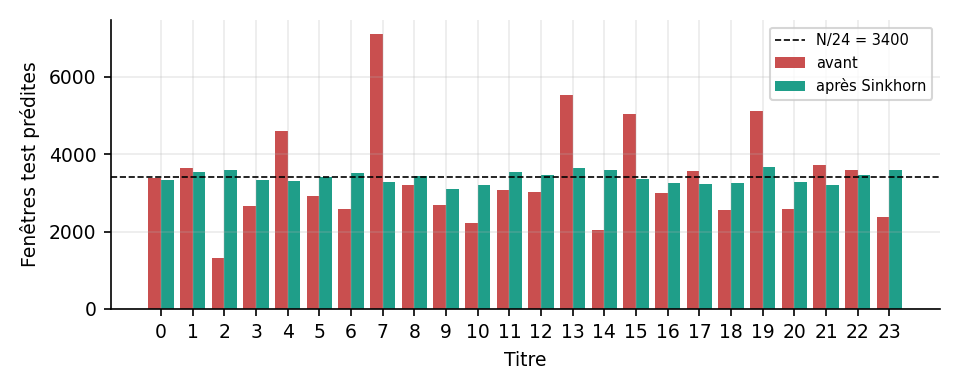
\includegraphics[width=.85\linewidth]{figures/sinkhorn_counts.png}
\caption{Fenêtres test prédites par titre, avant et après équilibrage (blend des 4 finalistes, refit).}
\label{fig:counts}
\end{figure}

\subsection{Rappel : correction de prior sous \emph{label shift}}
Supposons que seule la loi des classes change entre la source $s$ et la cible $\mathrm{t}$, et que $p_s(x\mid y)=p_{\mathrm{t}}(x\mid y)$. Par la formule de Bayes,
\begin{equation}
p_{\mathrm{t}}(y\mid x)=\frac{p(x\mid y)\pi_{\mathrm{t}}(y)}{\sum_{y'}p(x\mid y')\pi_{\mathrm{t}}(y')}
=\frac{p_s(y\mid x)\,\dfrac{\pi_{\mathrm{t}}(y)}{\pi_s(y)}}{\sum_{y'}p_s(y'\mid x)\,\dfrac{\pi_{\mathrm{t}}(y')}{\pi_s(y')}} .
\label{eq:labelshift}
\end{equation}
La correction optimale est donc un \emph{coefficient par classe} $w_y=\pi_{\mathrm{t}}(y)/\pi_s(y)$, suivi d'une renormalisation \cite{saerens,lipton}. Ici, $\pi_s$ est uniforme (6\,700 fenêtres par titre) et $\pi_{\mathrm{t}}$ l'est très probablement aussi. Le problème n'est donc pas un vrai label shift. Mais le covariate shift fait se comporter le modèle \emph{comme si} son prior implicite avait changé. On cherche les coefficients qui ramènent la masse prédite au prior visé.

\subsection{Formulation : projection entropique sur les marges}
Soit $P\in\R_{>0}^{N\times K}$ (probabilités strictement positives, écrêtées à $10^{-12}$), et $r=\1_N$, $c=\frac NK\1_K$ les marges visées. On cherche
\begin{equation}
Q^\star=\arg\min_{Q\ge0}\ \mathrm{KL}(Q\,\|\,P)=\sum_{i,k}Q_{ik}\log\frac{Q_{ik}}{P_{ik}}-Q_{ik}+P_{ik}
\quad\text{s.c.}\quad Q\1_K=r,\ \ Q^\top\1_N=c .
\label{eq:kl}
\end{equation}
\begin{proposition}[Forme de la solution]\label{prop:sinkform}
Il existe $u\in\R^N_{>0}$ et $w\in\R^K_{>0}$ tels que $Q^\star_{ik}=u_i\,P_{ik}\,w_k$.
\end{proposition}
\begin{proof}
Lagrangien : $\mathcal{L}=\mathrm{KL}(Q\|P)+\sum_i a_i(\sum_kQ_{ik}-1)+\sum_kb_k(\sum_iQ_{ik}-N/K)$. La condition de stationnarité donne $\partial\mathcal{L}/\partial Q_{ik}=\log(Q_{ik}/P_{ik})+a_i+b_k=0$, soit $Q_{ik}=P_{ik}e^{-a_i}e^{-b_k}$. On pose $u_i=e^{-a_i}$ et $w_k=e^{-b_k}$. Le problème est strictement convexe sur un polytope non vide (il contient $Q=\frac1K\1\1^\top$), donc la solution est unique.
\end{proof}

\begin{corollaire}[Règle de décision]
$\arg\max_kQ^\star_{ik}=\arg\max_kP_{ik}w_k$. Le facteur de ligne $u_i$ ne change pas la décision : l'équilibrage revient exactement à multiplier chaque titre par un coefficient $w_k$, comme dans~\eqref{eq:labelshift}.
\end{corollaire}

\begin{proposition}[Qui bascule]
La fenêtre $i$, prédite $c$ avant correction, est prédite $c'\neq c$ après si et seulement si
\begin{equation}
\frac{P_{ic'}}{P_{ic}}>\frac{w_c}{w_{c'}}\quad\text{et}\quad c'=\arg\max_kP_{ik}w_k .
\end{equation}
\end{proposition}
\noindent Une fenêtre confiante ($P_{ic}\gg P_{ic'}$) ne bascule que si le rapport des coefficients est extrême. Les fenêtres hésitantes basculent vers leur second choix. C'est ce qu'on observe (figure~\ref{fig:changed}).

\subsection{Algorithme de Sinkhorn--Knopp}
\begin{algo}[H]
\caption{\code{sinkhorn\_balance}}
\begin{algobox}
\item $Q\leftarrow\max(P,10^{-12})$.
\item Répéter 50 fois :
\begin{itemize}
\item[] colonnes : $Q_{ik}\leftarrow Q_{ik}\cdot\dfrac{N/K}{\sum_jQ_{jk}}$ ;
\item[] lignes : $Q_{ik}\leftarrow Q_{ik}\Big/\sum_{k'}Q_{ik'}$.
\end{itemize}
\item Retourner $Q$.
\end{algobox}
\end{algo}
Chaque étape est une projection de Bregman (en divergence KL) sur l'un des deux ensembles de contraintes affines. Pour une matrice strictement positive, les itérations convergent vers l'unique $Q^\star$ de la Proposition~\ref{prop:sinkform} \cite{sinkhorn,cuturi}. Les produits cumulés des facteurs de colonnes donnent $w$, ceux des facteurs de lignes donnent $u$.

\subsection{Exemple complet}
Quatre fenêtres, deux titres, vérité $(A,A,B,B)$.
\begin{center}\small
\begin{tabular}{cccccc}
\toprule
Fenêtre & Vrai & $P$ (A ; B) & avant & $Q^\star$ (A ; B) & après\\
\midrule
1 & A & 0,90 ; 0,10 & A & 0,838 ; 0,162 & A\\
2 & A & 0,70 ; 0,30 & A & 0,573 ; 0,427 & A\\
3 & B & 0,60 ; 0,40 & \old{A} & 0,463 ; 0,537 & \new{B}\\
4 & B & 0,20 ; 0,80 & B & 0,126 ; 0,874 & B\\
\midrule
\multicolumn{2}{c}{masse} & 2,40 ; 1,60 & 3/4 & 2,00 ; 2,00 & 4/4\\
\bottomrule
\end{tabular}
\end{center}
Coefficients obtenus : $w_B/w_A=1{,}739$. La fenêtre 3 bascule car $0{,}40/0{,}60=0{,}667>1/1{,}739=0{,}575$. La fenêtre 2 ne bascule pas : $0{,}30/0{,}70=0{,}43<0{,}575$.

\subsection{Effet observé sur le test}
\begin{figure}[H]\centering
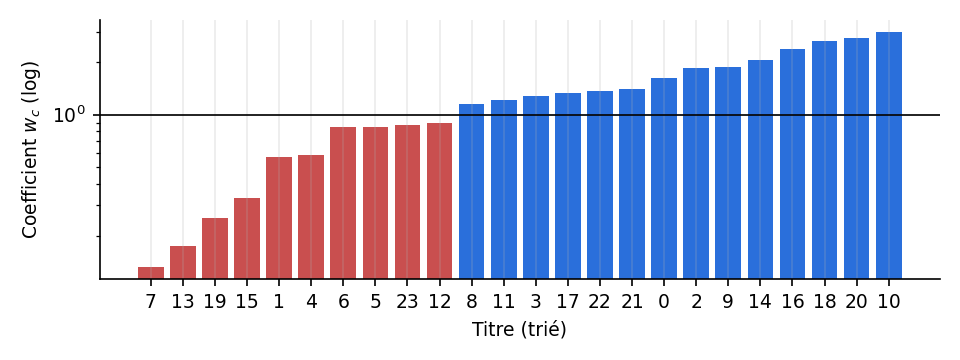
\includegraphics[width=.85\linewidth]{figures/sinkhorn_weights.png}
\caption{Coefficients $w_k$ (normalisés en moyenne géométrique). Titre 7 : $\times0{,}13$ ; titre 10 : $\times2{,}99$.}
\end{figure}
\begin{figure}[H]\centering
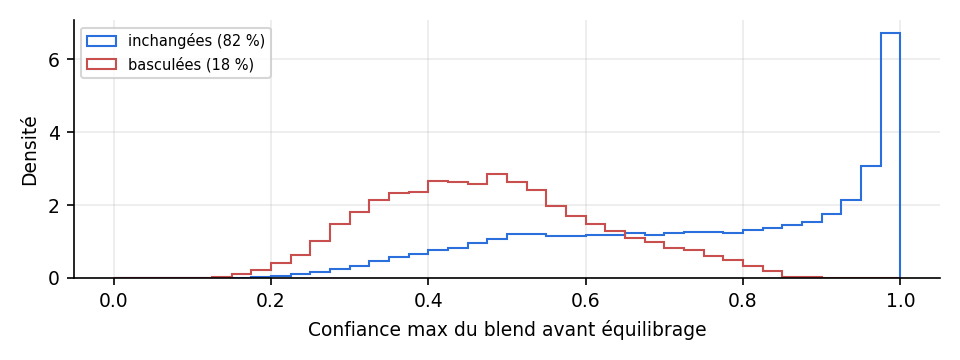
\includegraphics[width=.85\linewidth]{figures/sinkhorn_changed.png}
\caption{18\,\% des prédictions basculent. Leur confiance moyenne avant correction est de 0,48, contre 0,75 pour les fenêtres inchangées.}
\label{fig:changed}
\end{figure}

\begin{table}[H]\centering\small
\begin{tabular}{lccc}
\toprule
Blend des 4 finalistes & valid & stress & LB public\\
\midrule
brut & 0,8525 & 0,7411 & 0,5700\\
équilibré & 0,8599 & 0,8055 & \textbf{0,5958}\\
\midrule
gain & +0,7 pt & +6,4 pts & +2,6 pts\\
\bottomrule
\end{tabular}
\caption{L'équilibrage a été validé sur le stress \emph{avant} d'être soumis. Le stress, lui-même décalé en profondeur, a correctement prédit le signe du gain au LB, mais pas son ampleur.}
\end{table}

\subsection{Conditions de validité}
\begin{enumerate}
\item \textbf{Test équilibré.} Si $\pi_{\mathrm{t}}$ n'était pas uniforme, imposer $c=\frac NK\1$ dégraderait le score. Le gain observé au LB plaide pour l'uniformité, sans la démontrer.
\item \textbf{Bon classement relatif.} La correction ne change que l'importance relative des titres. Elle répare les fenêtres dont le bon titre est un second choix proche, pas les erreurs confiantes.
\item \textbf{Transductivité.} $w$ dépend de \emph{tout} le test. La prédiction d'une fenêtre dépend donc des autres fenêtres du test, et la conformité au règlement est à vérifier. Une variante non transductive consisterait à estimer $w$ sur un ensemble de référence (le stress, par exemple). Elle serait moins adaptée au vrai décalage.
\item \textbf{Différence avec Saerens et al.} \cite{saerens} \emph{estiment} $\pi_{\mathrm{t}}$ par EM :
\begin{equation}
\pi^{(k+1)}_c=\frac1N\sum_i\hat p^{(k)}_{ic},\qquad \hat p^{(k)}_{ic}\propto P_{ic}\,\pi^{(k)}_c/\pi_s(c).
\end{equation}
Nous \emph{imposons} au contraire que la masse prédite soit uniforme. C'est une hypothèse plus forte, adaptée à un test construit avec 20 fenêtres par titre et par jour.
\end{enumerate}

\section{Round 2 : voisins et indicateurs sans labels}\label{sec:voisins}

Ces outils ont été introduits en v0.2.0 (round 2), puis exécutés sur les vraies données en V3 : le vote entre voisins y fait passer le LB de $0{,}6028$ à $\mathbf{0{,}6351}$ (section~\ref{sec:v3}). Il reste dans toutes les soumissions suivantes, et sert aussi à construire le professeur de l'auto-apprentissage (section~\ref{sec:selftrain}). Cette section décrit la méthode ; les résultats sont à la section~\ref{sec:resultats}.

\subsection{Faire voter les fenêtres d'un même titre-jour}
Le test contient environ 20 fenêtres par titre et par jour, et elles partagent l'effet $\eta_{c,d}$ de~\eqref{eq:hier}. Le mécanisme qui gonflait la validation aléatoire (reconnaître le jour) peut être retourné en notre faveur : si une représentation $z$ rapproche les fenêtres d'un même titre-jour, une fenêtre ambiguë peut être corrigée par ses voisines plus nettes.

\paragraph{Graphe des $k$ plus proches voisins.} Pour un ensemble de fenêtres (le test entier, ou valid $\cup$ stress pour l'évaluation), on normalise $\hat z_i=z_i/\|z_i\|$, on note $\mathcal{N}_k(i)$ les $k$ indices maximisant $\hat z_i^\top\hat z_j$ avec $j\neq i$, et l'on forme $A_{ij}=\frac1k\ind{j\in\mathcal{N}_k(i)}$. Le calcul est exact, par blocs de 4\,096 lignes, sur GPU si disponible.

\paragraph{Propagation.} Pour $\alpha\in[0,1)$ :
\begin{equation}
Q^{(0)}=P,\qquad Q^{(n+1)}=(1-\alpha)P+\alpha AQ^{(n)} .
\end{equation}
\begin{proposition}
Pour $\alpha<1$, $Q^{(n)}\to Q^{(\infty)}=(1-\alpha)(I-\alpha A)^{-1}P$.
\end{proposition}
\begin{proof}
$A$ est stochastique par lignes, donc $\|A\|_\infty=1$ et $\|\alpha A\|_\infty<1$. L'itération est contractante, de point fixe unique $Q=(1-\alpha)P+\alpha AQ$. La série de Neumann $\sum_n(\alpha A)^n$ converge vers $(I-\alpha A)^{-1}$.
\end{proof}
\noindent C'est la propagation d'étiquettes de \cite{zhou}, appliquée à des probabilités \emph{prédites} plutôt qu'à des labels connus. Le code utilise 1 ou 5 itérations, puis renormalise les lignes et applique Sinkhorn.

\paragraph{Trois représentations.}
\begin{itemize}
\item \code{window} : blocs \code{levels}, \code{ticks}, \code{lots}, \code{cat\_freq} et \code{position}, standardisés à l'intérieur de l'ensemble. Ce sont justement des statistiques de régime : leur dérive nuit à la classification, mais elles identifient bien le jour.
\item \code{embedding} : $[z_{\text{seq}}\|z_{\text{ctx}}]$ des modèles, normalisé puis moyenné entre les membres. Les modèles de développement servent pour valid/stress, ceux du refit pour le test. Le code refuse d'utiliser les poids du refit sur des partitions étiquetées.
\item \code{probs} : $\sqrt{P}$, soit une distance de Hellinger.
\end{itemize}

\paragraph{Pureté.} Avant tout lissage, on mesure la part des voisins qui appartiennent au même titre :
\begin{equation}
\text{pureté}@k=\frac1{nk}\sum_i\sum_{j\in\mathcal{N}_k(i)}\ind{y_j=y_i}.
\end{equation}

\paragraph{Densité et facteur $k$.} Le pool d'évaluation valid $\cup$ stress contient $25\,\%$ des fenêtres de chaque jour, soit environ 5 par titre-jour, alors que le test en contient 20. Le $k$ choisi sur le pool est donc multiplié par $4$ pour le test. C'est une \emph{hypothèse}, écrite dans le code (\code{k\_scale}).

\paragraph{Règle d'adoption.} Le lissage n'est adopté que s'il améliore la précision \emph{équilibrée} sur le pool d'au moins $0{,}5$ point. Ce gain est un score de sélection, pas une estimation du gain sur le test.

\subsection{Test préliminaire : l'espace des probabilités ne suffit pas}\label{sec:probaspace}
Sur les probabilités réelles du run 1, avec des voisins dans l'espace \code{probs} :
\begin{center}\small
\begin{tabular}{lccc}
\toprule
pool valid $\cup$ stress & brut & équilibré & meilleur lissage + équilibrage\\
\midrule
précision & 0,8079 & 0,8281 & 0,8281\\
\bottomrule
\end{tabular}
\end{center}
C'était attendu : deux fenêtres voisines \emph{en probabilités} portent la même information, donc la propagation n'ajoute rien. L'intérêt du lissage dépend d'une représentation qui encode le \emph{jour}, ce que le round 2 mesure avec la pureté.

\subsection{Indicateurs sans labels sur le test}
Pour des probabilités test $P$ (modèle de développement) :
\begin{align}
\text{confiance}&=\tfrac1N\textstyle\sum_i\max_kP_{ik},\qquad
\text{entropie}=-\tfrac1N\sum_{i,k}P_{ik}\log P_{ik},\\
\text{KL d'équilibre}&=\textstyle\sum_k\hat\pi_k\log(K\hat\pi_k),\quad \hat\pi_k=\tfrac1N\sum_i\ind{\arg\max P_i=k},\\
\text{accord entre graines}&=\text{accord}(m,m')\ \text{pour deux graines d'une même configuration.}
\end{align}
Au run 1, pour \code{signature\_s0} :
\begin{center}\small
\begin{tabular}{lcc}
\toprule
& valid & test\\
\midrule
confiance & 0,858 & 0,738\\
accord entre graines & 0,845 & 0,648\\
plus grand / plus petit nombre de prédictions par titre & $\approx1$ & 5,4\\
\bottomrule
\end{tabular}
\end{center}
Ces chiffres annonçaient, avant toute soumission, que le test serait bien plus difficile que la validation. Ils ne sont pas des accuracies. Ils ne servent à présélectionner des modèles qu'une fois \emph{ancrés} à quelques scores LB connus.

\section{Résultats du run 1 (Kaggle, GPU)}\label{sec:resultats}

Les chiffres de cette section viennent des fichiers \code{lab\_results.zip} du run 1 (6 octobre 2026). Le split est fixé : fit 104\,520, valid 24\,120, stress 16\,080, audit 16\,080 (jamais ouvert).

\subsection{Screening univarié}
\begin{table}[H]\centering\small
\begin{tabular}{lccc}
\toprule
Feature & $\eta^2$ (fit) & KS train/test & shift (sd)\\
\midrule
\code{levels:log\_depth\_q90} & 0,630 & 0,135 & $-0{,}28$\\
\code{levels:log\_depth\_q50} & 0,618 & 0,170 & $-0{,}37$\\
\code{ticks:spread\_5p} & 0,563 & \new{0,024} & $-0{,}04$\\
\code{levels:log\_depth\_q10} & 0,510 & 0,174 & $-0{,}33$\\
\code{ticks:spread\_1} & 0,504 & \new{0,018} & $+0{,}03$\\
\code{ticks:log\_spread\_t\_mean} & 0,430 & \new{0,026} & $-0{,}06$\\
\code{levels:log\_absflux\_mean} & 0,415 & 0,172 & $-0{,}37$\\
\code{position:log\_dist\_mean} & 0,363 & 0,122 & $+0{,}31$\\
\code{lots:flux\_odd} & 0,361 & 0,191 & $+0{,}45$\\
\code{lots:flux\_round} & 0,353 & 0,183 & $-0{,}42$\\
\bottomrule
\end{tabular}
\caption{Les dix colonnes les plus séparatrices. En vert : les colonnes de tick, à la fois séparatrices et stables.}
\end{table}

\begin{figure}[H]\centering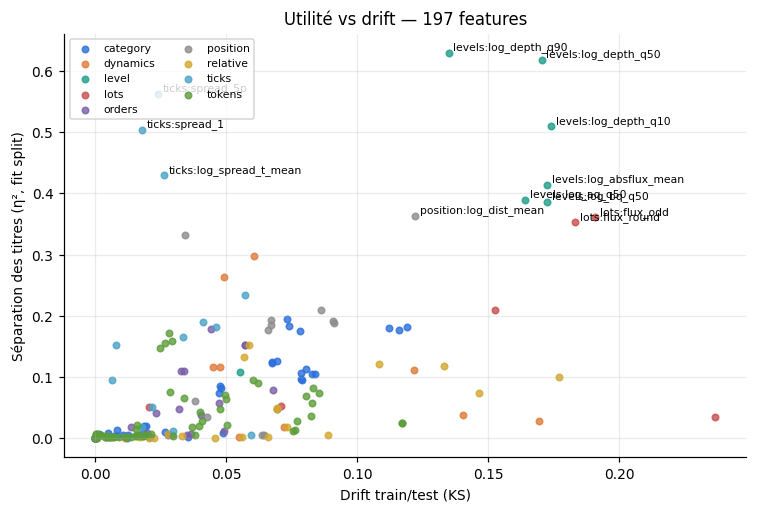
\includegraphics[width=.8\linewidth]{figures/screen_map.png}
\caption{Carte utilité/dérive des 197 colonnes.}\end{figure}

\paragraph{Trois enseignements.}
\begin{enumerate}
\item \textbf{Les ticks sont une signature stable.} $\eta^2\approx0{,}5$ avec $\mathrm{KS}\approx0{,}02$ : c'est exactement ce que la section~\ref{sec:unites} prédisait de la forme discrète du spread.
\item \textbf{La profondeur est séparatrice \emph{et} décalée.} Le test est moins profond de $0{,}3$ à $0{,}4$ écart-type.
\item \textbf{Les lots dérivent.} Le test contient davantage d'odd lots ($+0{,}45$ sd) et moins de lots ronds ($-0{,}42$ sd). Avec la baisse de profondeur, c'est cohérent avec l'hypothèse de prix plus élevés (section~\ref{sec:aug}).
\end{enumerate}

\subsection{AUC adversariale}
\begin{table}[H]\centering\small
\begin{tabular}{lcc|lcc}
\toprule
Bloc & $d$ & AUC & Bloc & $d$ & AUC\\
\midrule
\code{base\_relative} & 18 & 0,733 & \code{book\_dyn} & 10 & 0,669\\
\code{levels} & 7 & 0,709 & \code{cat\_cross} & 30 & 0,668\\
\code{lots} & 9 & 0,699 & \code{cat\_freq} & 12 & 0,668\\
\code{position} & 15 & 0,670 & \code{transitions} & 36 & 0,653\\
\code{tokens\_bow} & 24 & 0,618 & \code{orders} & 22 & 0,596\\
\code{ticks} & 14 & \new{0,568} & \textbf{tous} & 197 & \textbf{0,863}\\
\bottomrule
\end{tabular}
\caption{Séparabilité train/test, bloc par bloc. Le total (0,863) est cohérent avec l'ancienne AUC CatBoost (0,903). Aucun bloc seul n'explique le décalage : il est diffus.}
\end{table}
Fait notable : la base relative du pipeline précédent est \emph{la plus} décalée (0,733). Être invariant à l'échelle ne garantit pas d'être stable entre périodes.

\subsection{Ajout réentraîné}
Base \code{base\_relative}+\code{cat\_freq} : valid 0,313, stress 0,245 (XGBoost, 50\,\% du fit).
\begin{table}[H]\centering\small
\begin{tabular}{lrrrr}
\toprule
+ bloc & $\Delta$ valid & IC 95\,\% & $\Delta$ stress & retenu ?\\
\midrule
\code{position} & +5,9 & [+5,3 ; +6,4] & +3,8 & oui\\
\code{levels} & +5,4 & [+4,9 ; +5,9] & \old{$-13{,}3$} & \old{non}\\
\code{lots} & +5,2 & [+4,7 ; +5,8] & +4,3 & oui\\
\code{ticks} & +5,0 & [+4,5 ; +5,5] & \new{+5,3} & oui\\
\code{tokens\_bow} & +3,6 & [+3,1 ; +4,2] & +2,1 & oui\\
\code{book\_dyn} & +3,5 & [+3,0 ; +4,0] & $-0{,}1$ & oui\\
\code{transitions} & +2,0 & [+1,5 ; +2,5] & +1,7 & oui\\
\code{orders} & +1,5 & [+1,0 ; +1,9] & +0,8 & oui\\
\code{cat\_cross} & +0,6 & [+0,2 ; +1,1] & +0,4 & oui\\
\bottomrule
\end{tabular}
\caption{En points d'accuracy. \code{levels} est le seul bloc écarté par la règle : il fait gagner 5,4 points en validation et en perdre 13,3 en stress. C'est un piège de régime.}
\end{table}

\begin{figure}[H]\centering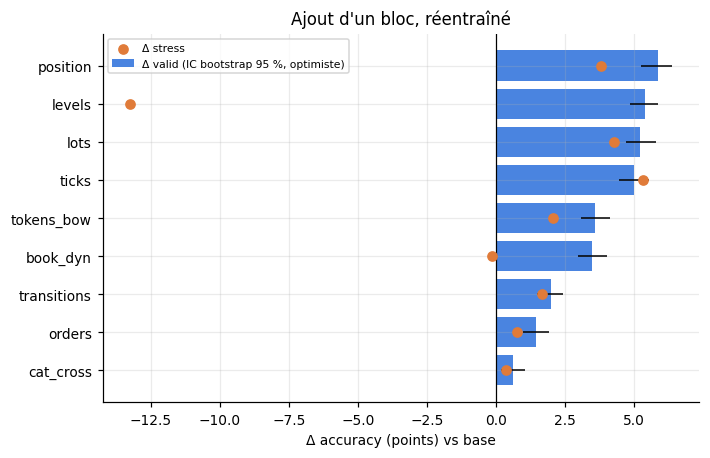
\includegraphics[width=.75\linewidth]{figures/screen_forward.png}\caption{Ajout réentraîné, valid et stress.}\end{figure}

\subsection{Retrait réentraîné}
Sur les 10 blocs retenus (190 colonnes) : valid 0,465, stress 0,364.
\begin{table}[H]\centering\small
\begin{tabular}{lrr|lrr}
\toprule
$-$ bloc & $\Delta$ valid & $\Delta$ stress & $-$ bloc & $\Delta$ valid & $\Delta$ stress\\
\midrule
\code{lots} & $-4{,}1$ & $-3{,}1$ & \code{book\_dyn} & $-0{,}7$ & $-0{,}1$\\
\code{base\_relative} & $-2{,}3$ & $-0{,}05$ & \code{transitions} & $-0{,}7$ & $-0{,}1$\\
\code{ticks} & $-1{,}4$ & $-1{,}6$ & \code{tokens\_bow} & $-0{,}4$ & $0{,}0$\\
\code{orders} & $-1{,}2$ & $-0{,}6$ & \code{cat\_freq} & $-0{,}2$ & $-0{,}3$\\
\code{position} & $-0{,}9$ & $-0{,}5$ & \code{cat\_cross} & $+0{,}1$ & $-0{,}2$\\
\bottomrule
\end{tabular}
\caption{En points. \code{cat\_cross}, \code{cat\_freq} et \code{tokens\_bow} sont redondants une fois les autres blocs présents.}
\end{table}

\subsection{Modèles}
\begin{table}[H]\centering\small
\begin{tabular}{lrrrrrr}
\toprule
Run & Param. & Ép. & Min & Valid & Stress & Stress éq.\\
\midrule
\code{tab\_lgbm} & — & 266 it. & 3,7 & 0,480 & 0,372 & —\\
\code{tab\_xgb} & — & 711 it. & 1,4 & 0,494 & 0,384 & —\\
\code{tab\_mlp} & — & 14 & 0,1 & 0,511 & 0,390 & —\\
\code{control\_gru\_s0} & 110\,105 & 39 & 3,2 & 0,787 & 0,662 & —\\
\code{signature\_relative\_only\_s0} & 340\,289 & 38 & 10,4 & 0,766 & 0,669 & —\\
\code{signature\_no\_bias\_s0} & 342\,905 & 40 & 8,6 & 0,824 & 0,716 & —\\
\code{signature\_s0} & 342\,913 & 38 & 10,4 & 0,825 & 0,712 & —\\
\code{signature\_s1} & 342\,913 & 37 & 10,4 & 0,827 & 0,730 & —\\
\code{signature\_robust\_s0} & 342\,913 & 39 & 10,5 & 0,830 & 0,689 & —\\
\code{signature\_robust\_s1} & 342\,913 & 35 & 10,5 & 0,836 & 0,719 & —\\
\midrule
\textbf{blend des 4 finalistes} & & & & 0,852 & 0,741 & 0,806\\
\bottomrule
\end{tabular}
\caption{Run 1. La colonne « stress éq. » (après Sinkhorn) n'a été calculée que pour le blend : elle devient le critère de sélection au round 2.}
\end{table}

\paragraph{Lecture prudente.}
\begin{itemize}
\item \textbf{Séquence contre tabulaire} : 0,79--0,84 contre 0,48--0,51 en validation. Lire les événements apporte beaucoup plus que des statistiques de fenêtre. Mais la validation aléatoire profite aussi davantage aux modèles séquentiels, qui reconnaissent mieux le jour (section~\ref{sec:dependance}).
\item \textbf{\code{signature} contre \code{control\_gru}} : +3,8 points en valid, +5,0 en stress. Mais le rapport de paramètres est de $3{,}1$. Design et capacité sont confondus : c'est l'objet de \code{gru\_wide} au round 2.
\item \textbf{Biais « même ordre »} : 0,8251 avec, 0,8238 sans. L'écart est plus petit que celui entre graines (0,8251 et 0,8266). Pas d'effet mesurable : le retirer simplifie le modèle.
\item \textbf{Robustesse} (venue dropout, jitter, dropout de blocs) : +0,7 point en valid en moyenne, $-1{,}7$ en stress. Pas de gain de transfert.
\item \textbf{Niveaux} : les retirer coûte 5,9 points en valid et 4,3 en stress (une seule graine).
\item \textbf{Maturité} : la meilleure époque tombe entre 35 et 40, mais c'est la fin du cosinus qui aplatit la courbe. L'écart en mode \code{eval} est de 0,91 (train) contre 0,82 (valid).
\end{itemize}

\begin{figure}[H]\centering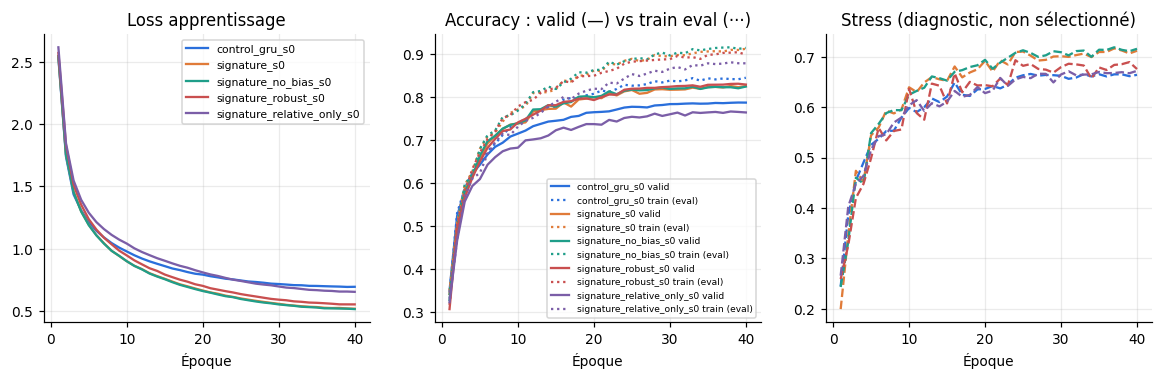
\includegraphics[width=\linewidth]{figures/histories.png}\caption{Courbes d'apprentissage (seed 0). Le stress est tracé mais ne sélectionne rien.}\end{figure}
\begin{figure}[H]\centering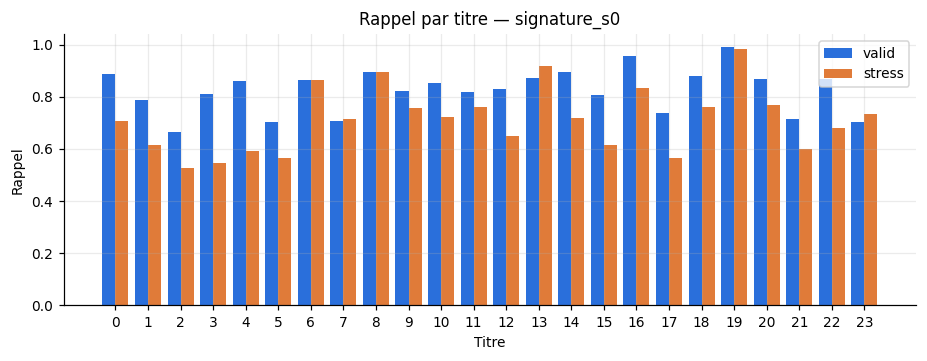
\includegraphics[width=.9\linewidth]{figures/recall_signature_s0.png}\caption{Rappel par titre, \code{signature\_s0}.}\end{figure}

\subsection{Du stress au leaderboard}
\begin{figure}[H]\centering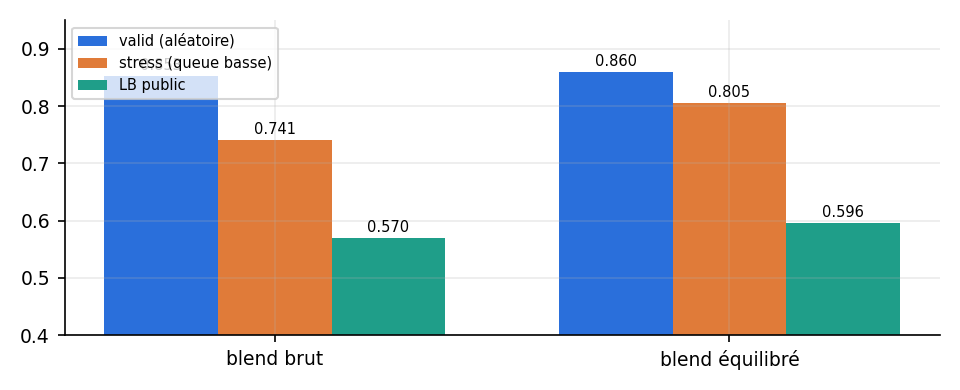
\includegraphics[width=.75\linewidth]{figures/valid_stress_lb.png}
\caption{Les trois mesures pour les deux soumissions. Le classement relatif (brut < équilibré) est le même partout. L'écart absolu, lui, ne l'est pas.}\end{figure}
L'écart validation → LB est de 28 points. L'écart stress → LB est de 17 points (brut) et de 21 points (équilibré). Aucune partition interne n'estime donc le score public. En revanche, le stress a correctement \emph{ordonné} les deux variantes. C'est pourquoi le round 2 classe les configurations sur le stress équilibré, et ancre les indicateurs sans labels sur les deux scores connus.

\section{Démonstration contrôlée : 25 modèles, un seul protocole}\label{sec:demo}

Les sections précédentes décrivent des runs qui changeaient plusieurs choses à la fois. Le notebook \code{v\_demo/CFM\_demo\_models} reprend le projet de zéro, avec des modèles volontairement simples (chacun moins de 20 minutes sur GPU) et un protocole \emph{identique} pour tous : même cache, mêmes partitions (fit, valid par grappes de régime, stress = carnets les moins profonds), mêmes métriques. Son but n'est pas de battre le LB. Il sert à \emph{attribuer} chaque gain à une seule cause. Toutes les mesures sont internes, sans pseudo-labels, donc sans la contamination de la section~\ref{sec:contam}.

\begin{figure}[H]\centering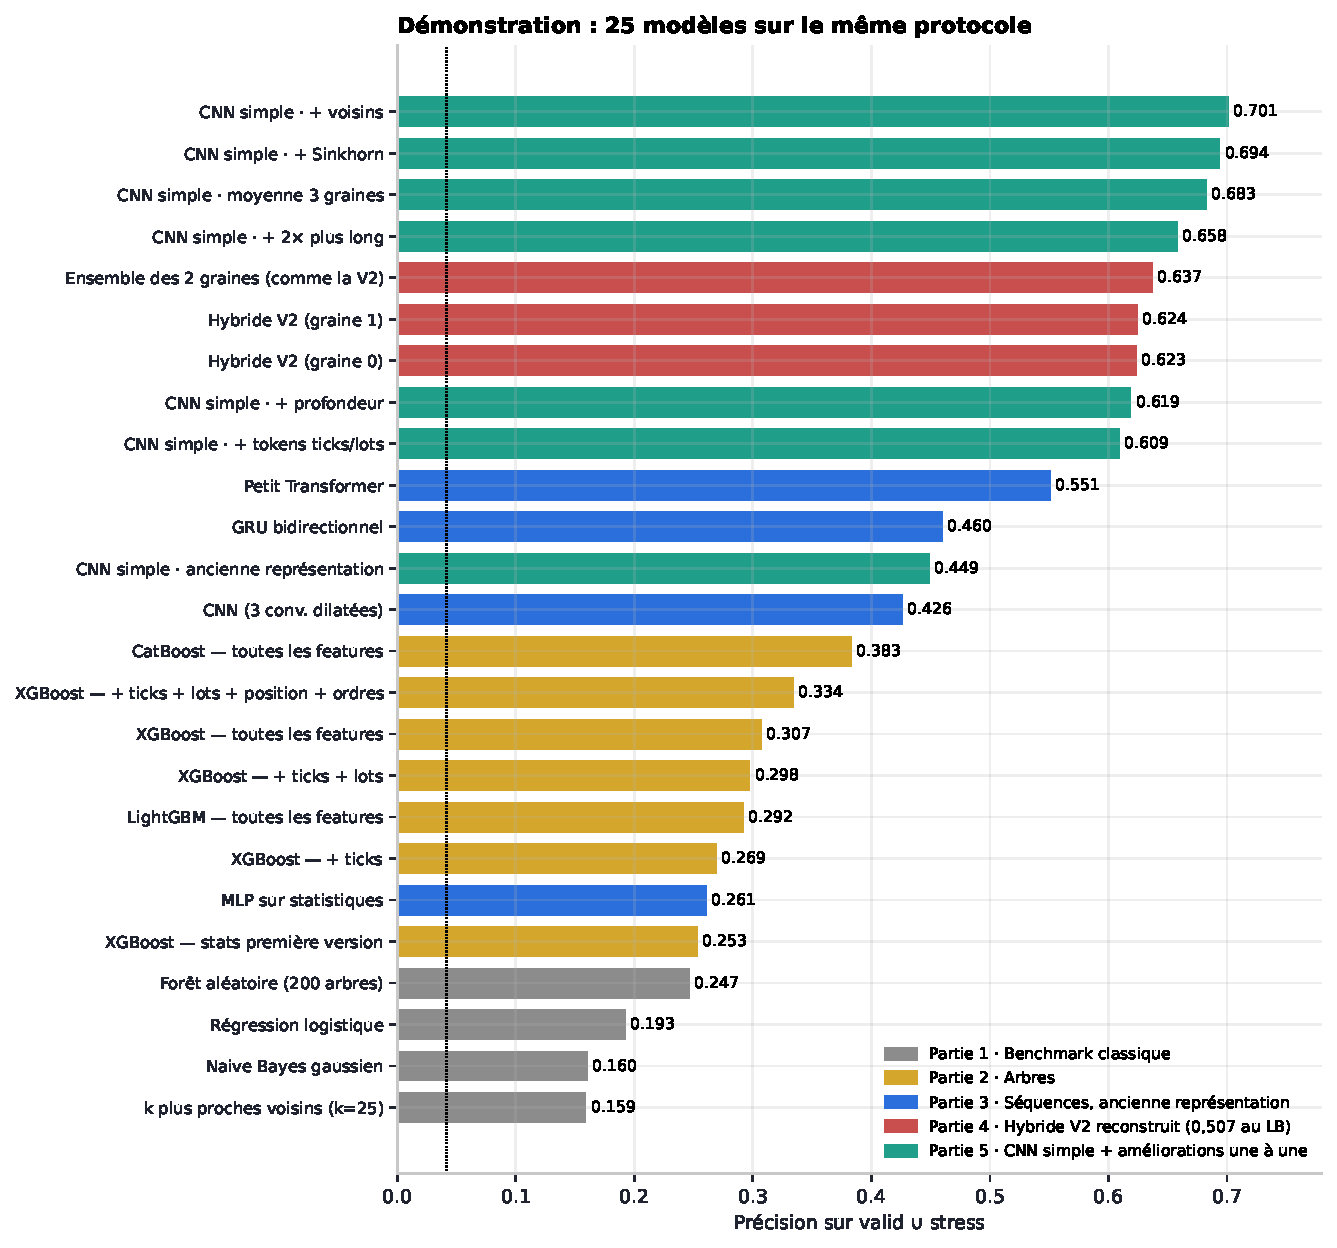
\includegraphics[width=.86\linewidth]{figures/demo_synthese.pdf}
\caption{Les 25 modèles du notebook, classés par précision sur valid $\cup$ stress. Pour les parties 1 à 4, c'est la moyenne pondérée des précisions équilibrées valid et stress. Pour la partie 5, c'est la précision mesurée directement sur l'union (équilibrée à partir de l'étape Sinkhorn). Un petit CNN d'environ 100\,k paramètres, nourri des tokens en ticks et en lots, dépasse la reconstruction de l'ancien meilleur modèle dès qu'on l'entraîne plus longtemps.}
\label{fig:demo-synth}\end{figure}

\subsection{Parties 1 et 2 : modèles classiques et arbres}
\begin{figure}[H]\centering
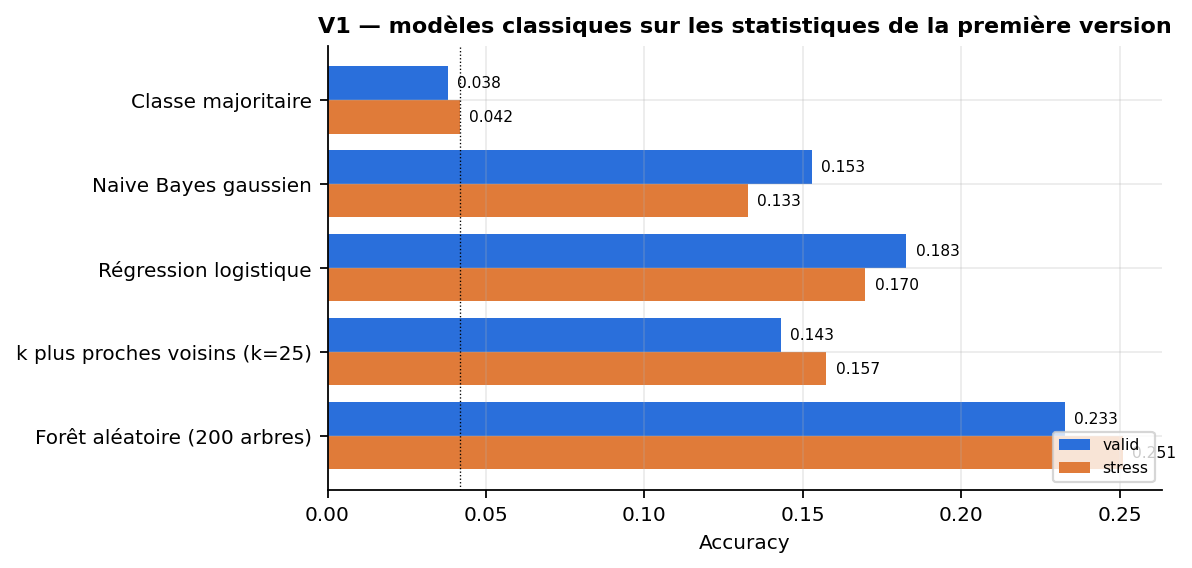
\includegraphics[width=.49\linewidth]{figures/demo_v1_compare.png}\hfill
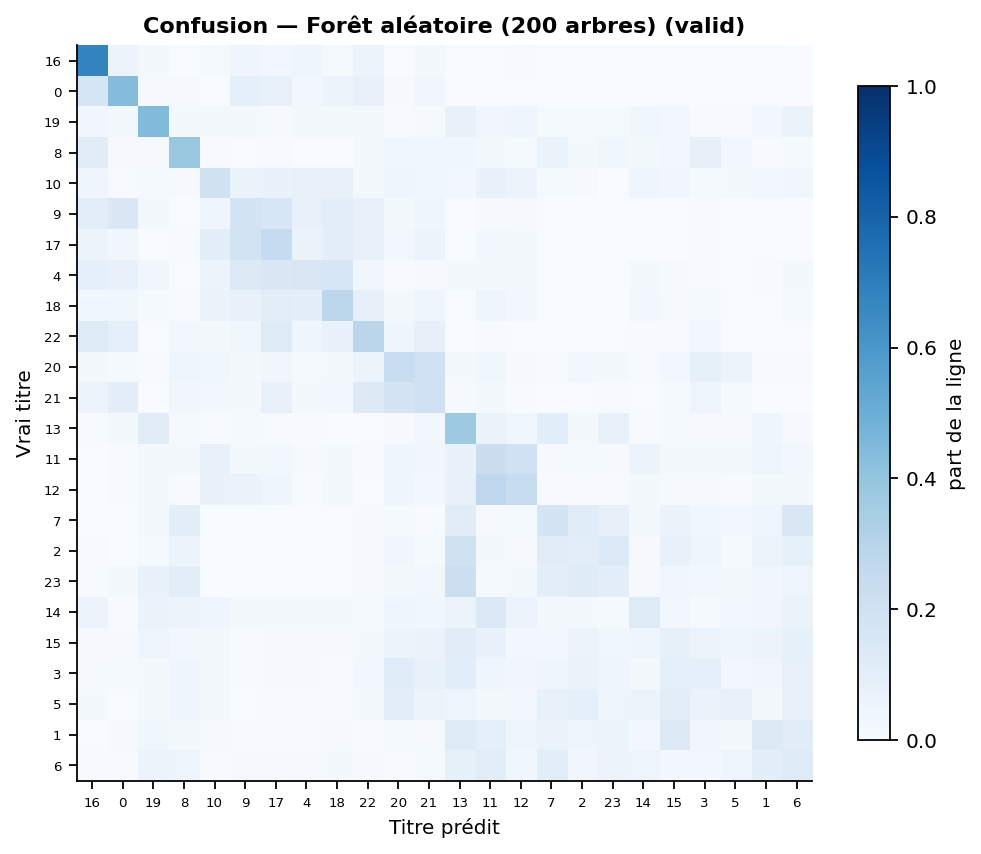
\includegraphics[width=.44\linewidth]{figures/demo_v1_confusion.png}
\caption{Partie 1. Modèles classiques sur les statistiques de fenêtre de la toute première version. Le meilleur, une forêt aléatoire, plafonne à 0,23 en valid et 0,25 en stress, avec une confusion diffuse : ces statistiques ne portent presque pas la signature des titres.}
\end{figure}

\begin{figure}[H]\centering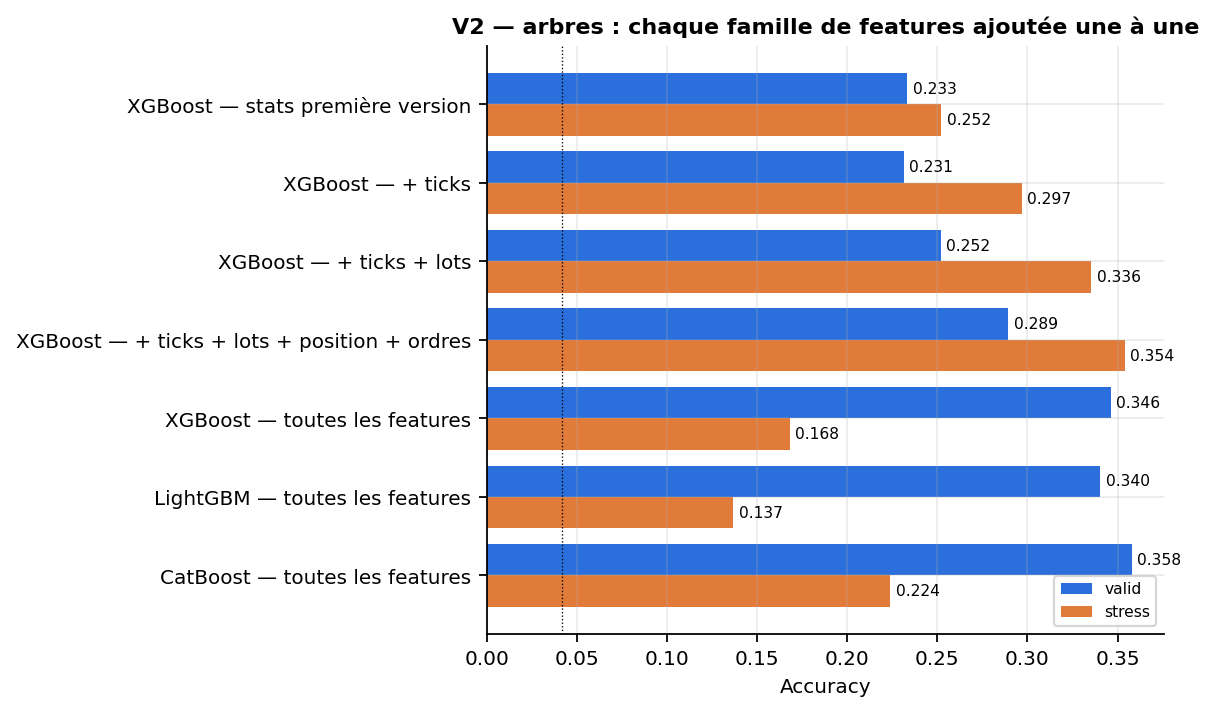
\includegraphics[width=.75\linewidth]{figures/demo_v2_compare.png}
\caption{Partie 2. XGBoost en ajoutant une famille de features à la fois. Les familles stables font monter le \emph{stress} à chaque ajout : 0,252 (statistiques initiales), 0,297 (+ ticks), 0,336 (+ lots), 0,354 (+ position et ordres). Avec \emph{toutes} les features, profondeur comprise, la valid monte à 0,346 mais le stress s'effondre à 0,168 (0,137 pour LightGBM, 0,224 pour CatBoost). C'est le piège de régime de la section~\ref{sec:screening}, reproduit ici sur trois implémentations différentes.}
\label{fig:demo-trees}\end{figure}

\begin{figure}[H]\centering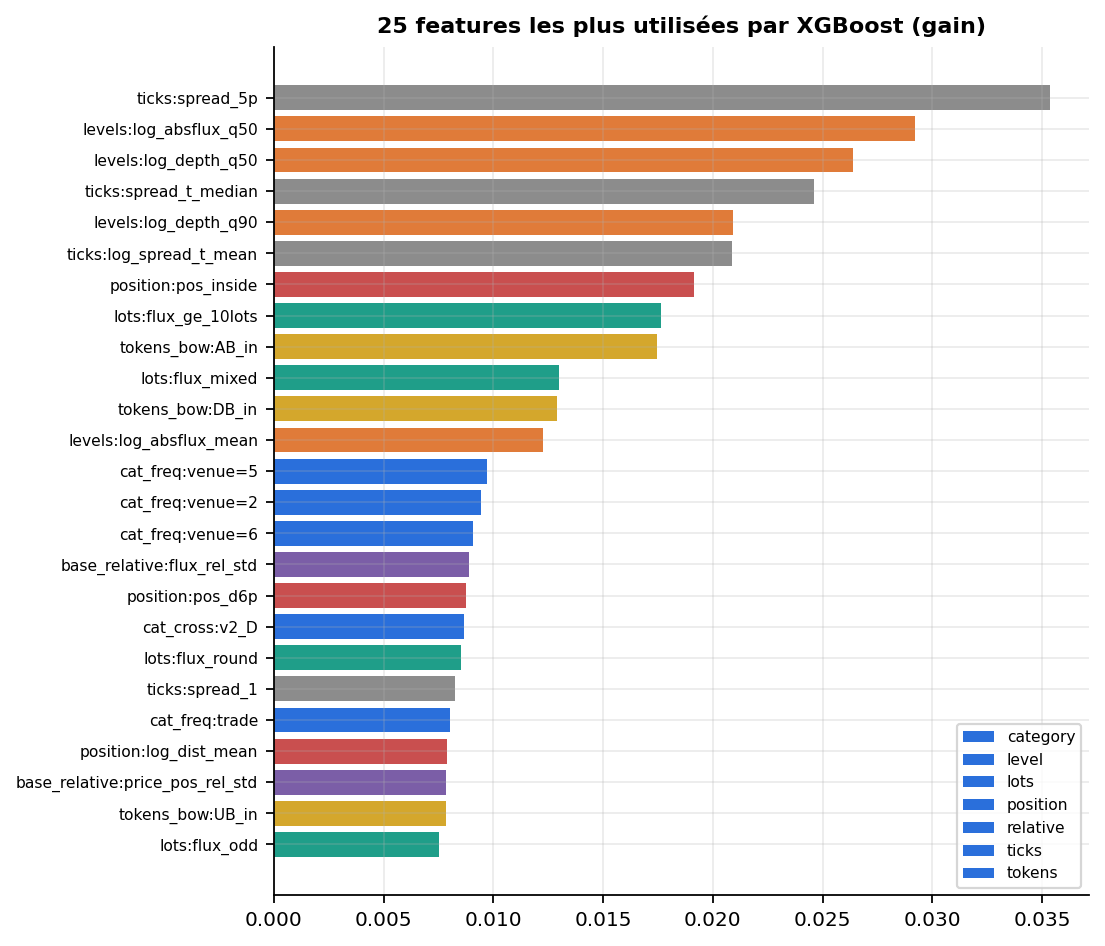
\includegraphics[width=.7\linewidth]{figures/demo_v2_importance.png}
\caption{Les 25 features les plus utilisées par XGBoost (gain). En tête, le spread en ticks (\code{ticks:spread\_5p}), la signature stable, mais juste derrière, trois mesures de profondeur. Un arbre exploite tout ce qui sépare sur la période d'entraînement, sans distinguer signature et régime : c'est exactement ce que la figure~\ref{fig:demo-trees} fait payer en stress.}
\end{figure}

\subsection{Parties 3 et 4 : lire la séquence, et l'ancien record}
\begin{figure}[H]\centering
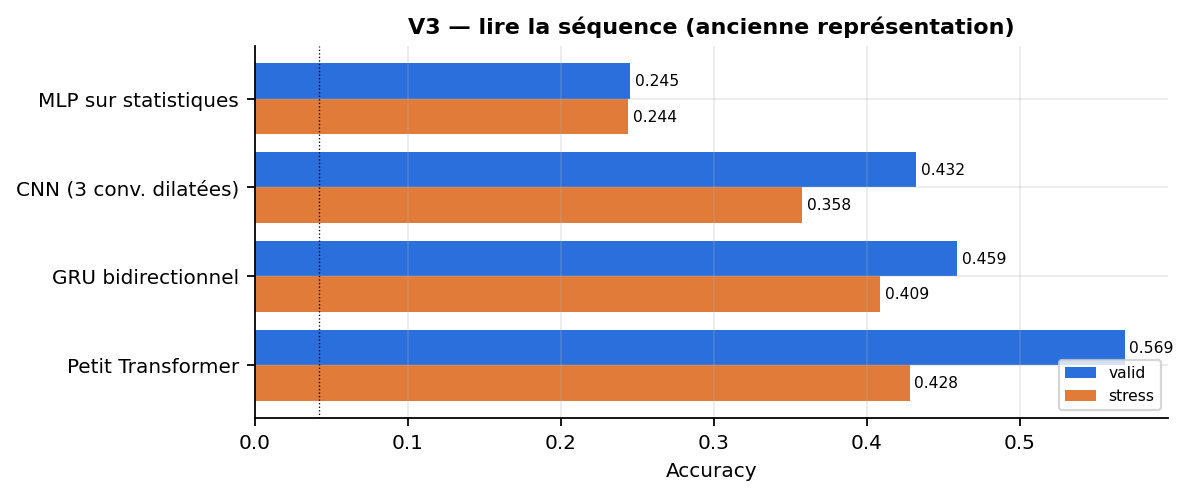
\includegraphics[width=.47\linewidth]{figures/demo_v3_compare.png}\hfill
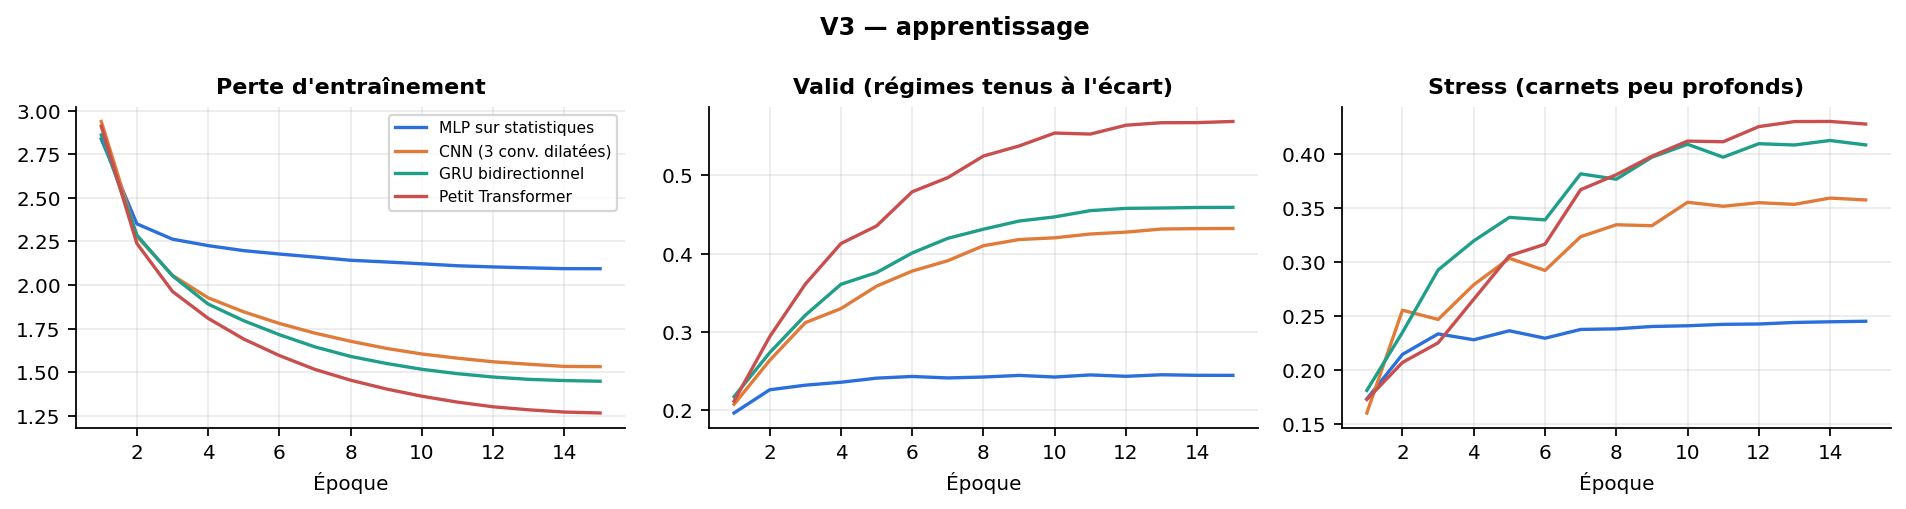
\includegraphics[width=.51\linewidth]{figures/demo_v3_curves.png}
\caption{Partie 3. Quatre réseaux sur l'\emph{ancienne} représentation relative. Lire la séquence plutôt que des résumés fait passer la valid de 0,245 (MLP sur statistiques) à 0,432 (CNN), 0,459 (GRU bidirectionnel) et 0,569 (petit Transformer). Même avec de mauvaises unités, l'ordre des événements porte beaucoup d'information.}
\end{figure}

\begin{figure}[H]\centering
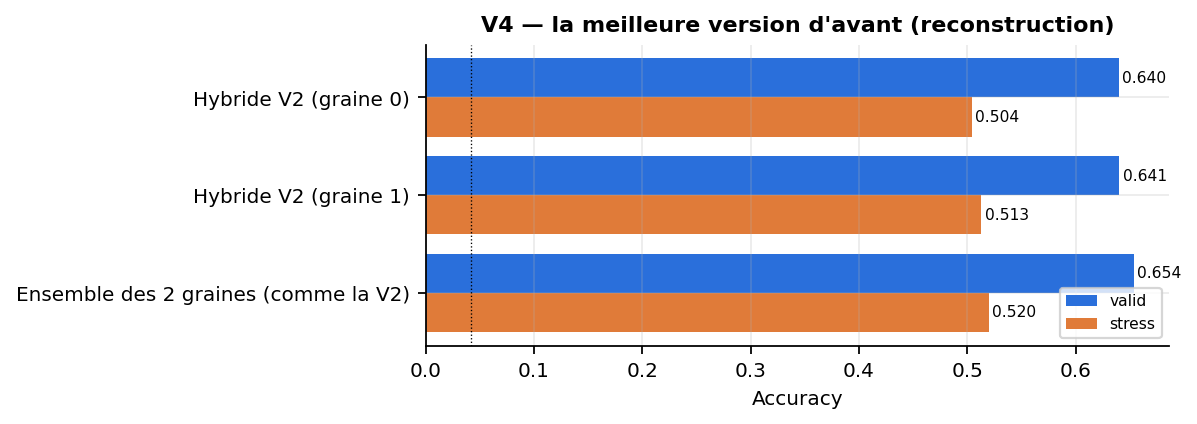
\includegraphics[width=.47\linewidth]{figures/demo_v4_compare.png}\hfill
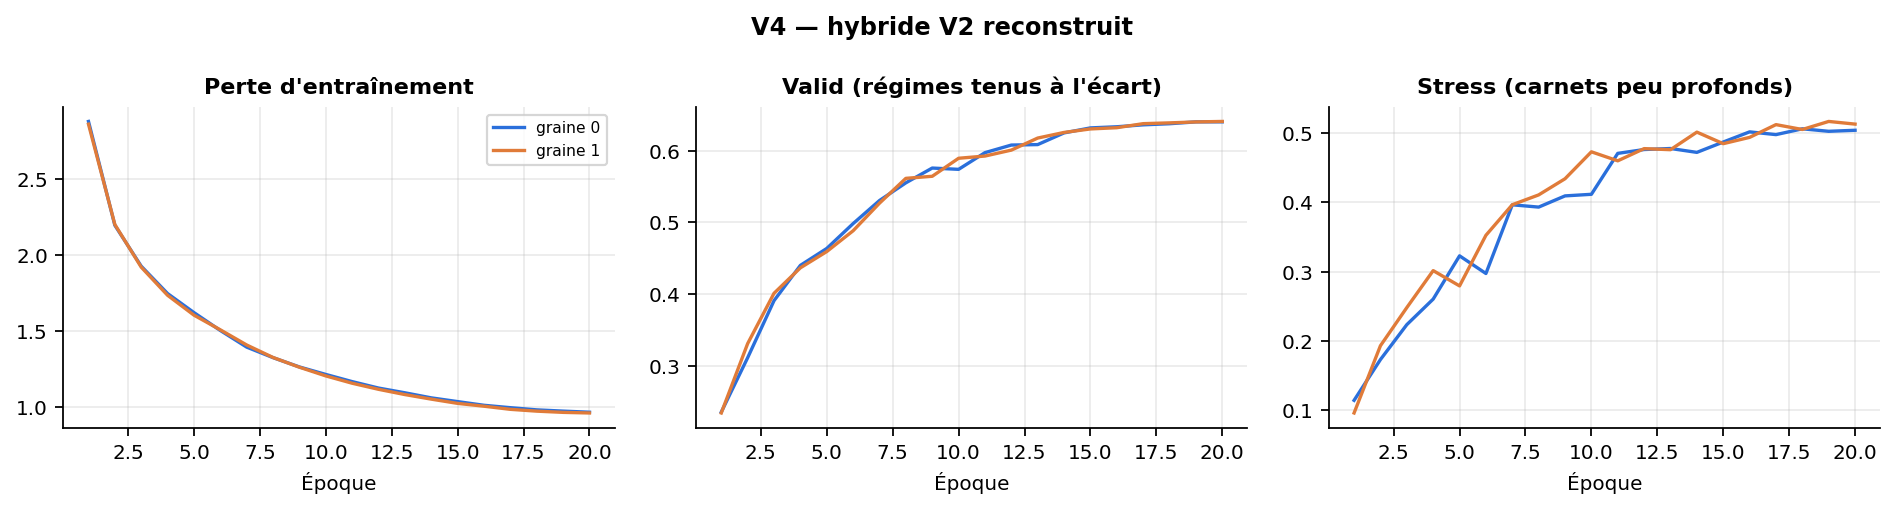
\includegraphics[width=.51\linewidth]{figures/demo_v4_curves.png}
\caption{Partie 4. Reconstruction simplifiée du Transformer hybride de la V2, le record historique à 0,507 au LB. Deux graines donnent 0,640--0,641 en valid et 0,504--0,513 en stress, l'ensemble 0,654 et 0,520. Fait notable : le stress brut de ce modèle (0,52) est très proche de son score public (0,507), alors que la valid le surestime de 15 points.}
\label{fig:demo-v2}\end{figure}

\subsection{Partie 5 : les améliorations, une à la fois}
On part d'un petit CNN (trois convolutions dilatées, environ 100\,k paramètres) qui lit l'ancienne représentation, puis on ajoute \emph{une seule} chose à chaque étape, toujours mesurée sur les mêmes 42\,627 fenêtres de valid $\cup$ stress.

\begin{table}[H]\centering\small
\begin{tabular}{clcc}
\toprule
Étape & Ajout & Précision valid $\cup$ stress & Gain\\
\midrule
0 & ancienne représentation (20 époques) & 0,449 & —\\
1 & \textbf{tokens en ticks et en lots} & 0,609 & \textbf{+16,0}\\
2 & augmentation de profondeur ($\sigma=0{,}3$) & 0,619 & +1,0\\
3 & entraînement deux fois plus long (40 époques) & 0,658 & +3,9\\
4 & moyenne de 3 graines & 0,683 & +2,5\\
5 & équilibrage de Sinkhorn & 0,694 & +1,1\\
6 & vote entre voisins (\code{combo}, $k=10$, $\alpha=0{,}5$, 5 it.) & \textbf{0,701} & +0,7\\
\bottomrule
\end{tabular}
\caption{L'échelle de la partie 5. Les étapes 5 et 6 n'utilisent que le pool lui-même (voisins cherchés dans valid $\cup$ stress), sans le test.}
\label{tab:ladder}\end{table}

\begin{figure}[H]\centering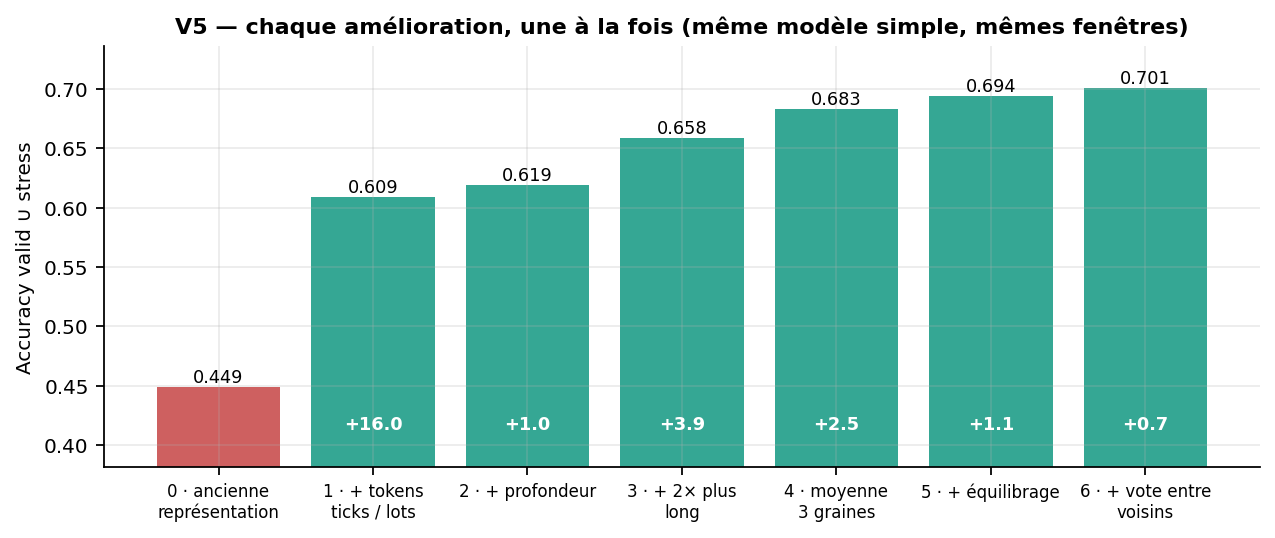
\includegraphics[width=.85\linewidth]{figures/demo_v5_ladder.png}
\caption{L'échelle de la table~\ref{tab:ladder} en image. À comparer avec la progression publique de la figure~\ref{fig:lb} : les leviers arrivent dans le même ordre d'importance, à une exception près. Le vote entre voisins rapporte peu en interne (+0,7) et beaucoup au LB (+3,2), parce que le test contient quatre fois plus de fenêtres par titre-jour que le pool.}
\end{figure}

\paragraph{Ce que l'échelle établit.} La section~\ref{sec:limites} notait que les $+6{,}3$ points du premier run mêlaient représentation, architecture et ensemble. L'étape 1 isole la représentation : \emph{même} réseau, \emph{même} entraînement, \emph{mêmes} fenêtres. Passer de l'ancienne représentation relative aux tokens en ticks et en lots vaut à elle seule \textbf{+16 points} internes, plus que toutes les autres étapes réunies (+9,2). C'est la mesure la plus nette du projet en faveur de la thèse des unités naturelles. Elle reste interne : son ampleur au LB n'est pas mesurée.

\begin{figure}[H]\centering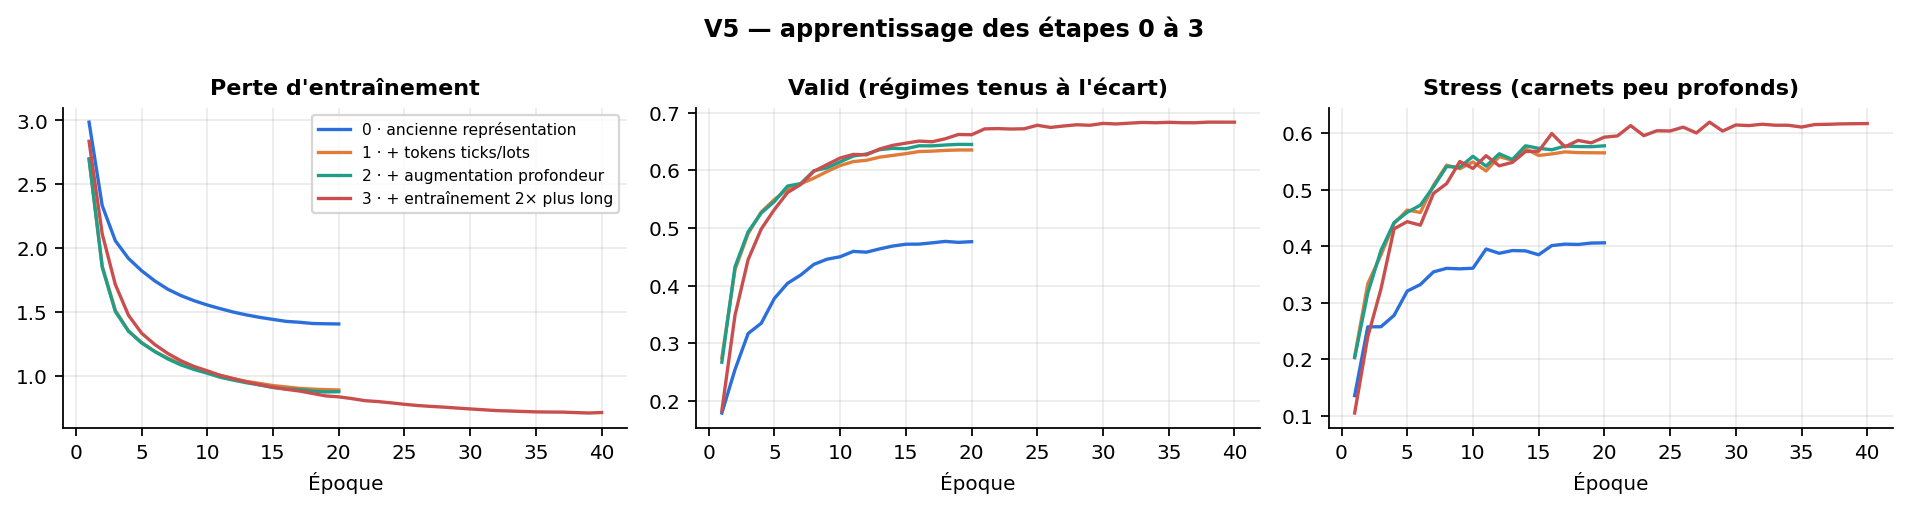
\includegraphics[width=\linewidth]{figures/demo_v5_curves.png}
\caption{Courbes d'apprentissage des étapes 0 à 3. L'ancienne représentation (bleu) plafonne vers 0,47 en valid. Toutes les variantes à tokens montent plus vite et plus haut. L'entraînement long (rouge) continue de progresser jusqu'à l'époque 40.}
\end{figure}

\begin{figure}[H]\centering
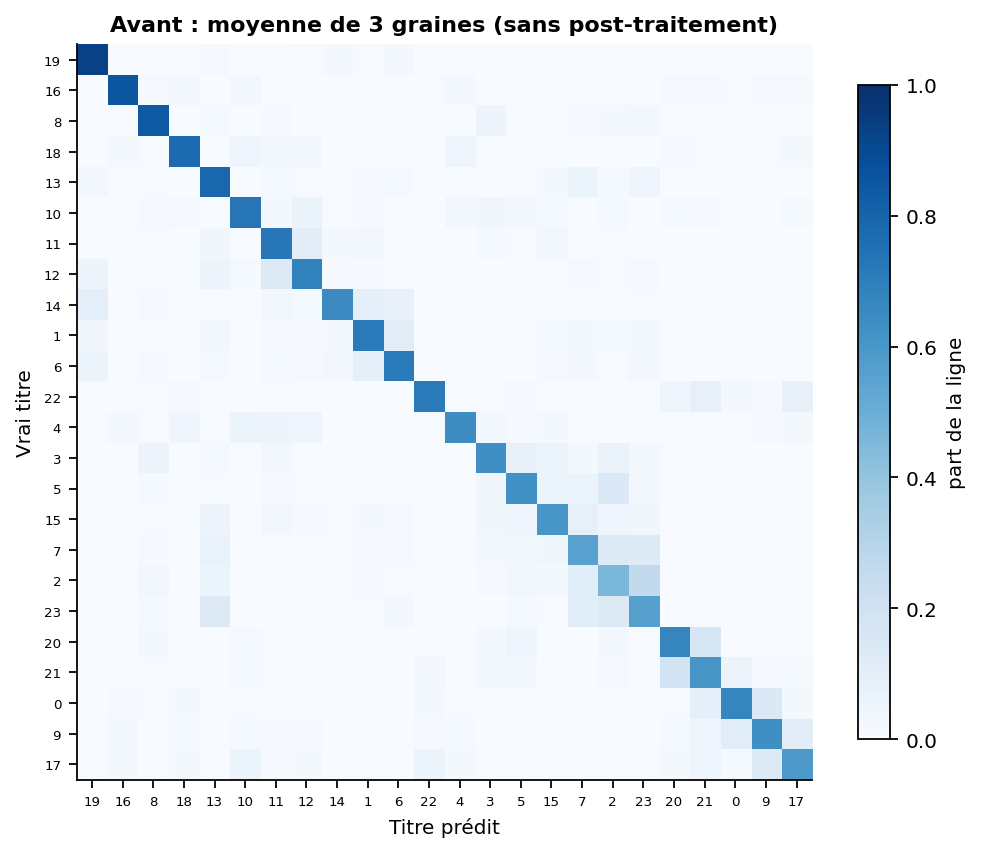
\includegraphics[width=.49\linewidth]{figures/demo_v5_confusion_before.png}\hfill
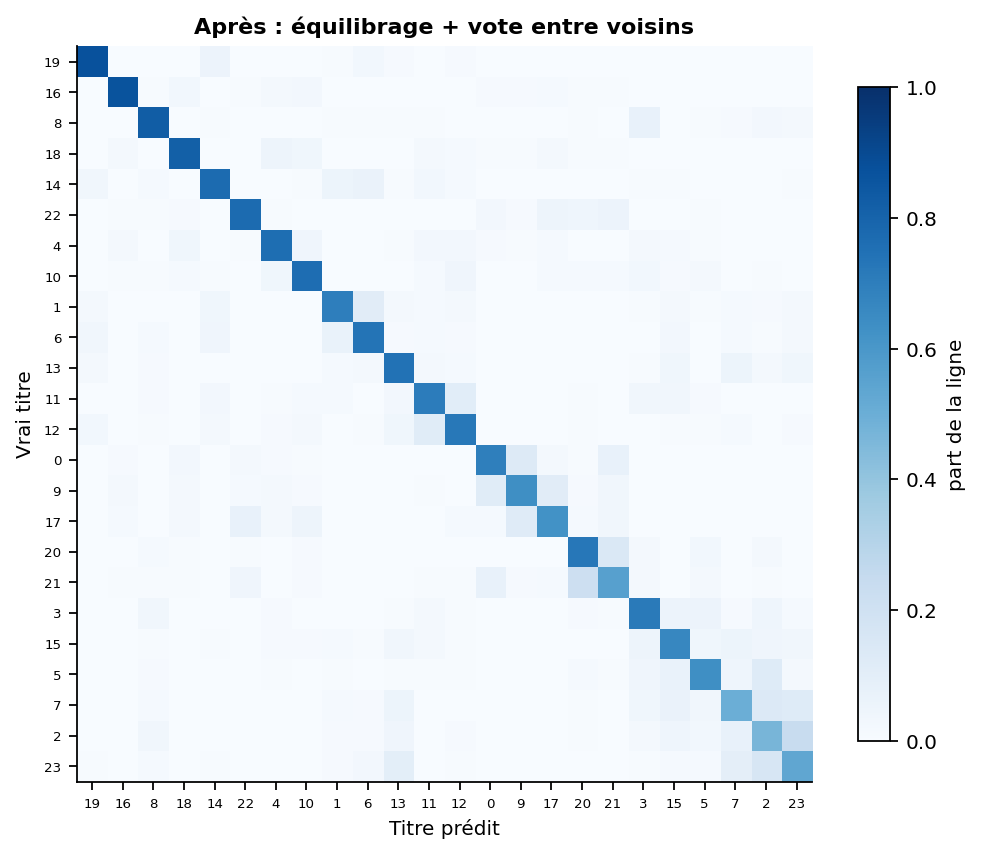
\includegraphics[width=.49\linewidth]{figures/demo_v5_confusion_after.png}
\caption{Confusions du CNN simple sur le stress, avant (moyenne de 3 graines) et après (équilibrage + vote entre voisins). Les erreurs restantes se concentrent dans les mêmes familles que pour le grand modèle, $\{20,21\}$, $\{2,7,23\}$, $\{0,9,17\}$ : elles tiennent à la donnée plus qu'au modèle.}
\end{figure}

\begin{figure}[H]\centering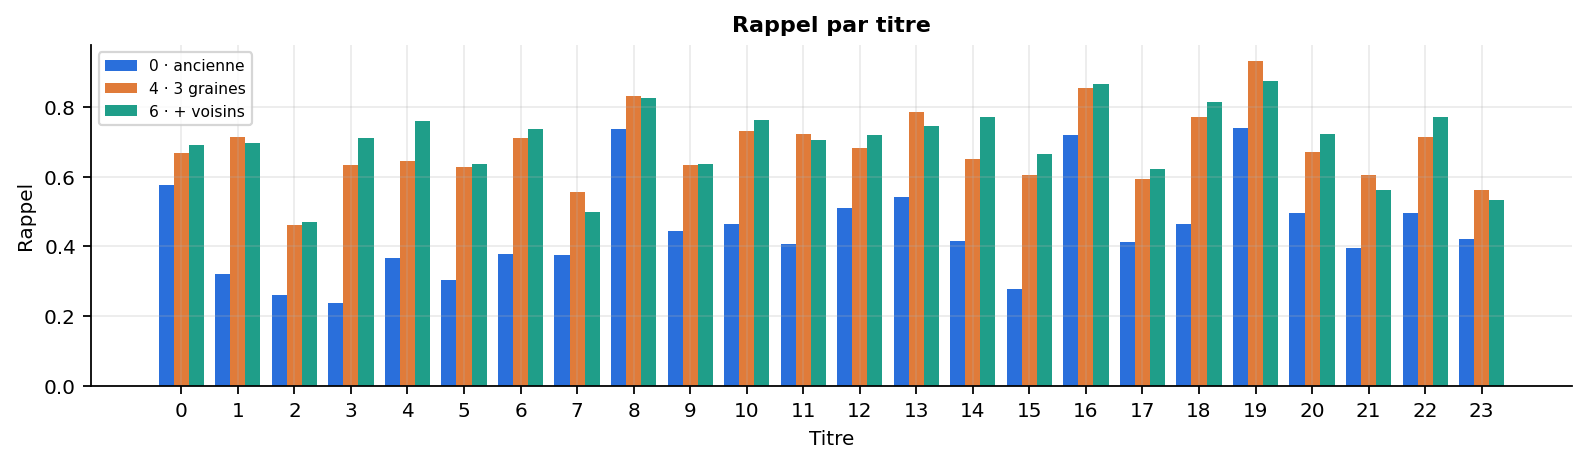
\includegraphics[width=.9\linewidth]{figures/demo_v5_recall.png}
\caption{Rappel par titre : ancienne représentation (étape 0), 3 graines (étape 4), après voisins (étape 6). Le gain est général, il ne vient pas de quelques titres faciles. Les plus gros sauts concernent des titres que l'ancienne représentation ne reconnaissait presque pas (1, 3, 5, 15 : de 0,25--0,3 à plus de 0,6).}
\end{figure}

\begin{figure}[H]\centering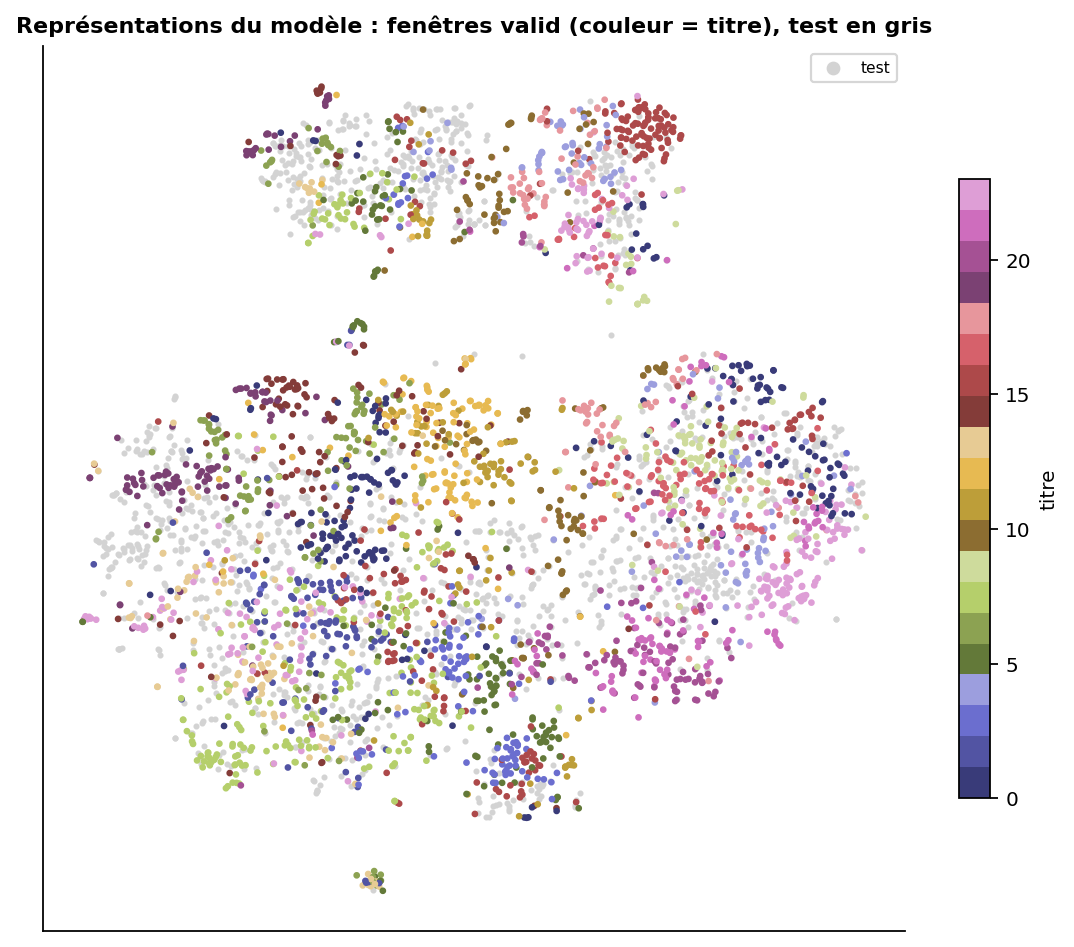
\includegraphics[width=.62\linewidth]{figures/demo_v5_tsne.png}
\caption{Représentations internes du CNN simple (t-SNE) : fenêtres valid colorées par titre, fenêtres test en gris. Le test occupe les mêmes régions que la valid, sans îlot isolé : la représentation transfère d'une période à l'autre, ce qui rend le vote entre voisins et l'auto-apprentissage possibles.}
\end{figure}

\subsection{Ce que la démonstration ajoute}
\begin{enumerate}
\item \textbf{Une attribution propre.} À architecture égale, la représentation vaut +16 points internes. Ce n'était qu'une conjecture dans la section~\ref{sec:resultats}.
\item \textbf{Un modèle simple suffit.} Un CNN de 100\,k paramètres, sans attention, atteint 0,683 avant tout post-traitement, contre 0,637 pour la reconstruction de l'ancien record. L'essentiel du gain tient à la donnée et au protocole, pas à la complexité du réseau.
\item \textbf{Le piège de régime est robuste.} Trois implémentations d'arbres le reproduisent : ajouter les features de profondeur fait gagner en valid et perdre en stress.
\end{enumerate}

\section{V4 et V5 : auto-apprentissage transductif}\label{sec:selftrain}

Après la V3, chaque brique transductive (équilibrage, alignement, voisins) agissait \emph{au moment de la prédiction} : le modèle restait celui de la période d'entraînement, et l'on corrigeait ses sorties. L'auto-apprentissage va plus loin : il \emph{réentraîne} le modèle sur des fenêtres de la période test, étiquetées par un modèle précédent. C'est l'idée du \emph{pseudo-label}~\cite{lee} et de l'élève bruité~\cite{xie}, appliquée ici à un changement de période plutôt qu'à des données non étiquetées de même loi. Deux tours ont été joués. Le premier (V4) prend V3~B comme professeur, le second (V5) prend V4~C. Ils font passer le score public de $0{,}6351$ à $\mathbf{0{,}6835}$, soit le plus gros gain cumulé du projet après la représentation initiale.

\begin{figure}[H]\centering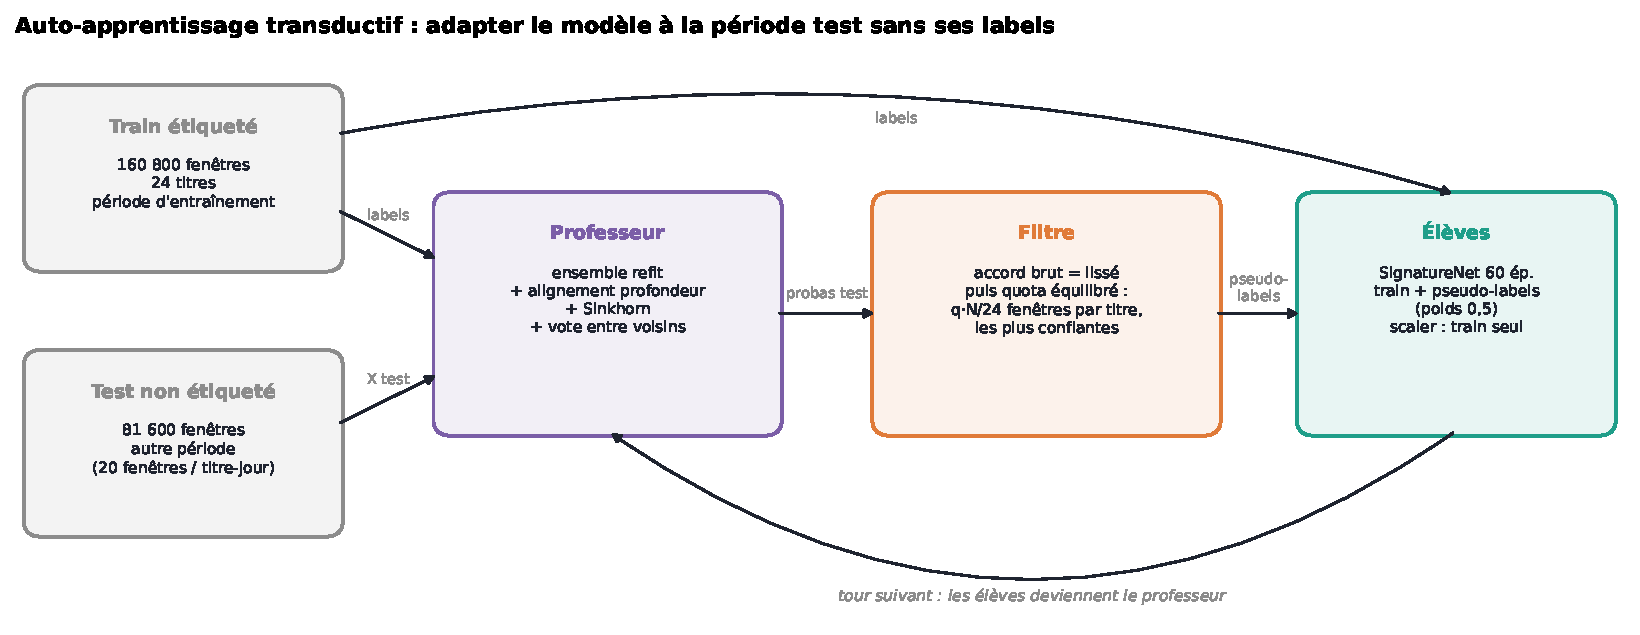
\includegraphics[width=\linewidth]{figures/v5_self_training_loop.pdf}
\caption{La boucle d'auto-apprentissage. Le professeur étiquette les fenêtres test où ses deux lectures concordent ; un quota par titre empêche de transmettre son biais de classes ; les élèves s'entraînent sur train $\cup$ pseudo-labels, puis deviennent le professeur du tour suivant.}
\label{fig:loop}\end{figure}

\subsection{Formalisation}

\paragraph{Les deux lectures du professeur.} Soit $\mathcal{T}$ l'ensemble des $N=81\,600$ fenêtres test. Le professeur fournit deux matrices de probabilités sur $\mathcal{T}$ :
\begin{itemize}
\item la lecture \emph{brute} $P^{\text{brut}}=\mathrm{Sinkhorn}\big(\tfrac1M\sum_{m}P^{(m)}\big)$, moyenne équilibrée de ses $M$ membres ;
\item la lecture \emph{lissée} $Q=\mathrm{Sinkhorn}\big(Q^{(5)}\big)$, après le vote entre voisins de la section~\ref{sec:voisins}. C'est la soumission elle-même.
\end{itemize}
On note $\hat y_i=\arg\max_c Q_{ic}$ et $\kappa_i=\max_c Q_{ic}$ la confiance.

\begin{definition}[Fenêtres éligibles]
$\mathcal{E}=\{i\in\mathcal{T} : \arg\max_c Q_{ic}=\arg\max_c P^{\text{brut}}_{ic}\}$.
\end{definition}
\noindent Les deux lectures n'utilisent pas la même information. $P^{\text{brut}}$ ne regarde que la fenêtre $i$. $Q$ regarde aussi ses voisines du même titre-jour. Exiger leur accord revient à demander deux « vues » concordantes, dans l'esprit du co-apprentissage~\cite{blum} : une fenêtre dont le label ne tient qu'au vote de ses voisines, ou qu'à sa seule lecture isolée, est écartée. Le désaccord touche 9,1\,\% du test en V4 et 7,9\,\% en V5.

\begin{definition}[Quota équilibré]
Pour une part $q\in(0,1)$, soit $m=\lfloor qN/K\rfloor$. Pour chaque titre $c$, on retient les $m$ fenêtres de $\mathcal{E}\cap\{\hat y=c\}$ de plus grande confiance $\kappa_i$ :
\begin{equation}
\mathcal{S}_q=\bigcup_{c=1}^{K}\operatorname{top}_m\big(\{i\in\mathcal{E} : \hat y_i=c\},\ \kappa\big).
\end{equation}
\end{definition}

\begin{remarque}[Pourquoi un quota plutôt qu'un seuil]
Un seuil $\kappa_i\ge\tau$ retient davantage de fenêtres dans les titres faciles. Le prior empirique des pseudo-labels hérite alors du biais du professeur, et l'élève le renforce. Avec le quota, $|\mathcal{S}_q\cap\{\hat y=c\}|=m$ pour tout $c$, dès que chaque titre a au moins $m$ fenêtres éligibles. C'est le cas dans les deux tours : en V5, le titre le moins fourni compte 2\,795 éligibles pour un quota de 2\,040 à $q=0{,}6$. Le prior des pseudo-labels est donc exactement uniforme, ce qui est cohérent avec l'hypothèse d'un test équilibré déjà utilisée par Sinkhorn (section~\ref{sec:sinkhorn}).
\end{remarque}

\paragraph{Emboîtement.} Comme la sélection se fait par confiance décroissante à l'intérieur de chaque titre, $q<q'\Rightarrow\mathcal{S}_q\subseteq\mathcal{S}_{q'}$. Le contrôle $q=0{,}4$ de la V5 est donc un sous-ensemble strict de la sélection $q=0{,}6$ : les deux élèves ne diffèrent que par les 16\,320 fenêtres les moins sûres.

\paragraph{Perte de l'élève.} Soit $\mathcal{D}$ les fenêtres étiquetées utilisées pour l'entraînement (le fit en développement, tous les labels au refit). L'élève minimise, sur chaque lot $B\subset\mathcal{D}\cup\mathcal{S}_q$, la moyenne pondérée
\begin{equation}
\mathcal{L}_B(\theta)=\frac{\sum_{j\in B}w_j\,\ell_\varepsilon\big(f_\theta(x_j),\tilde y_j\big)}{\sum_{j\in B}w_j},\qquad
(w_j,\tilde y_j)=\begin{cases}(1,\,y_j) & j\in\mathcal{D}\\ (\omega,\,\hat y_j) & j\in\mathcal{S}_q\end{cases}
\end{equation}
où $\ell_\varepsilon$ est l'entropie croisée avec lissage des labels et $\omega=0{,}5$. Deux garde-fous complètent la formule. La standardisation du contexte est estimée sur les seules fenêtres étiquetées, pour que les statistiques du test n'entrent pas par ce biais. Le fichier de pseudo-labels est vérifié par empreinte et par alignement sur les \code{obs\_id} du test : un run ne peut pas être réutilisé avec d'autres pseudo-labels.

\begin{algo}[H]
\caption{Un tour d'auto-apprentissage}\label{alg:selftrain}
\begin{algobox}
\item Entrées : probabilités brute $P^{\text{brut}}$ et lissée $Q$ du professeur sur le test ; part $q$ ; poids $\omega$.
\item $\mathcal{E}\leftarrow\{i : \arg\max Q_i=\arg\max P^{\text{brut}}_i\}$.
\item Pour chaque titre $c$ : garder les $\lfloor qN/K\rfloor$ fenêtres de $\mathcal{E}$ prédites $c$ de plus grande confiance $\Rightarrow\mathcal{S}_q$, labels $\hat y$.
\item Entraîner $S$ graines de SignatureNet (60 époques, configuration \code{v3\_long}) sur fit $\cup\,\mathcal{S}_q$ ; sélectionner l'époque sur valid.
\item Refit de chaque graine sur tous les labels $\cup\,\mathcal{S}_q$, même nombre d'époques.
\item Prédire le test, alignement de profondeur si adopté, moyenne, vote entre voisins, Sinkhorn $\Rightarrow$ nouveau $Q$.
\item Le nouvel ensemble devient le professeur du tour suivant.
\end{algobox}
\end{algo}

\subsection{La mesure interne est contaminée}\label{sec:contam}
\begin{proposition}
Les précisions valid et stress d'un élève sont biaisées vers le haut par rapport à celles d'un modèle sans pseudo-labels, indépendamment de tout gain de transfert.
\end{proposition}
\begin{proof}[Argument]
Le professeur est un ensemble \emph{refit}, entraîné sur tous les labels, valid et stress compris. Ses pseudo-labels $\hat y$ sont donc des fonctions de $y_{\text{valid}}$ et $y_{\text{stress}}$. En apprenant $\hat y$ sur des fenêtres test proches des fenêtres valid (même titre, régime voisin), l'élève reçoit indirectement une partie de l'information de leurs labels. Son score valid n'est plus celui d'un modèle qui n'a jamais vu ces labels.
\end{proof}
\noindent L'ampleur du biais est inconnue. Elle croît avec $q$ : plus de pseudo-labels transmettent plus d'information. Conséquence pratique : dans cette section, les mesures internes servent à vérifier que l'entraînement s'est bien passé. Les gains se lisent \emph{uniquement} au LB, à l'aide de soumissions de contrôle qui ne diffèrent que d'un élément.

\subsection{V4 : le premier tour et son contrôle}
\paragraph{Pseudo-labels.} Le professeur est V3~B (0,6351). Ses lectures brute (V3~A) et lissée concordent sur 90,9\,\% du test. Avec $q=0{,}4$, on retient 32\,640 fenêtres, 1\,360 par titre, de confiance moyenne 0,813 et minimale 0,455.

\begin{table}[H]\centering\small
\begin{tabular}{lcccc}
\toprule
Configuration & Graines & Valid éq. & Stress éq. & Meilleure époque\\
\midrule
\code{v3\_long} (ancre, 60 époques) & 2 & 0,785 & 0,791 & 54--58\\
\code{v4\_xlong} (90 époques) & 3 & 0,797 & 0,800 & 55--90\\
\code{v4\_student} (\code{v3\_long} + pseudo-labels, $q=0{,}4$) & 2 & \textbf{0,814} & \textbf{0,815} & 49--59\\
\bottomrule
\end{tabular}
\caption{V4, modèles seuls (Sinkhorn appliqué à chacun). Les élèves sont en partie contaminés (section~\ref{sec:contam}).}
\end{table}

\begin{table}[H]\centering\small
\begin{tabular}{llc}
\toprule
Soumission & Contenu & LB public\\
\midrule
V3 B (référence) & 6 modèles à 60 époques, alignement, Sinkhorn, voisins & 0,6351\\
\textbf{V4 C} & \code{v4\_xlong} $\times3$ + élèves $\times2$, $\gamma=1{,}239$, Sinkhorn, voisins ($k=40$) & \textbf{0,6551}\\
V4 D (contrôle) & \code{v4\_xlong} $\times3$ seuls, mêmes post-traitements & \old{0,6174}\\
\bottomrule
\end{tabular}
\caption{Le contrôle D isole les élèves. C $-$ D $=+3{,}8$ points : tout le gain de la V4 leur revient.}
\end{table}

\paragraph{Deux lectures du contrôle.}
\begin{enumerate}
\item \textbf{L'entraînement long ne transfère pas.} En interne, 90 époques gagnent $+1{,}1$ point sur 60. Au LB, D est $1{,}8$ point \emph{sous} V3~B. C'est la première fois dans le projet qu'un gain interne change de signe au LB. Deux causes restent confondues : le surapprentissage de la période d'entraînement (figure~\ref{fig:curves}, la log-loss valid de \code{v4\_xlong} ne baisse plus après l'époque 40) et un ensemble deux fois plus petit (3 modèles contre 6).
\item \textbf{Les élèves corrigent les fenêtres qu'on ne leur a pas données.} C et D sont d'accord sur 98,9\,\% des fenêtres pseudo-étiquetées, mais sur 81,5\,\% seulement des 60\,\% restantes. Le gain de C ne vient donc pas d'une copie du professeur. Les élèves ont appris des traits propres à la période test et les ont étendus aux fenêtres les plus difficiles. C'est de l'adaptation de domaine.
\end{enumerate}

\subsection{V5 : un second tour, un meilleur professeur}
\paragraph{Hypothèses, fixées avant le run.} H1 : un professeur meilleur (V4~C, 0,6551) donne de meilleurs pseudo-labels, donc de meilleurs élèves. H2 : passer de $q=0{,}4$ à $q=0{,}6$ donne plus de signal sur la période test. Ce signal porte sur les fenêtres non étiquetées, là où la V4 a gagné. Les modèles longs sont abandonnés.

\paragraph{Pseudo-labels.} Les lectures brute et lissée de V4~C concordent sur 92,1\,\% du test.
\begin{table}[H]\centering\small
\begin{tabular}{lccccc}
\toprule
Quota & Fenêtres & Par titre & Titres sous le quota & Confiance min. & Confiance moy.\\
\midrule
$q=0{,}4$ & 32\,640 & 1\,360 & 0 & 0,544 & 0,849\\
$q=0{,}6$ & 48\,960 & 2\,040 & 0 & 0,456 & 0,791\\
\bottomrule
\end{tabular}
\caption{Sélections V5. Elles sont emboîtées : la sélection à 40\,\% est incluse dans celle à 60\,\%.}
\end{table}

\begin{figure}[H]\centering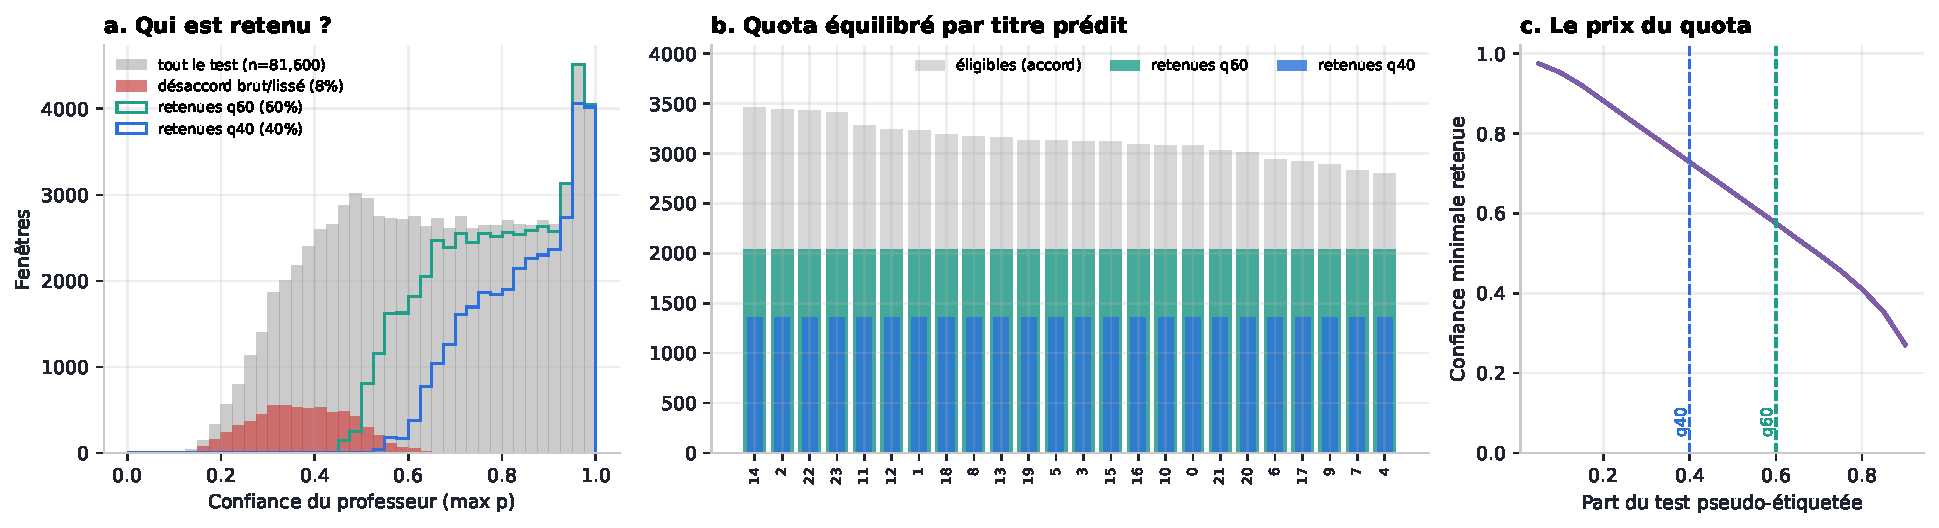
\includegraphics[width=\linewidth]{figures/v5_pseudo_selection.pdf}
\caption{Sélection des pseudo-labels V5. (a) Les fenêtres où les deux lectures divergent ont une confiance faible (mode vers 0,3) : le filtre écarte bien les cas douteux. (b) Le quota coupe les titres sur-prédits : chaque titre reçoit exactement 2\,040 (resp. 1\,360) fenêtres. (c) Confiance minimale atteinte si l'on étendait la sélection sans quota. Elle chute rapidement au-delà de 60\,\%, ce qui borne l'intérêt d'aller plus loin.}
\label{fig:pseudo}\end{figure}

\paragraph{Élèves.}
\begin{table}[H]\centering\small
\begin{tabular}{lccccc}
\toprule
Configuration & Graines & Valid éq. & Stress éq. & Accord test avec V4 C & Minutes\\
\midrule
\code{v5\_q40} & 3 & 0,813 $\pm$ 0,003 & 0,815 $\pm$ 0,001 & 0,787 & 16,0\\
\code{v5\_q60} & 3 & \textbf{0,823} $\pm$ 0,000 & \textbf{0,826} $\pm$ 0,000 & 0,826 & 17,7\\
\bottomrule
\end{tabular}
\caption{V5, modèles seuls (moyenne $\pm$ écart-type entre graines). L'écart q60 $-$ q40 ($+1$ point) est compatible avec une contamination plus forte et ne prouve pas H2.}
\end{table}

\begin{figure}[H]\centering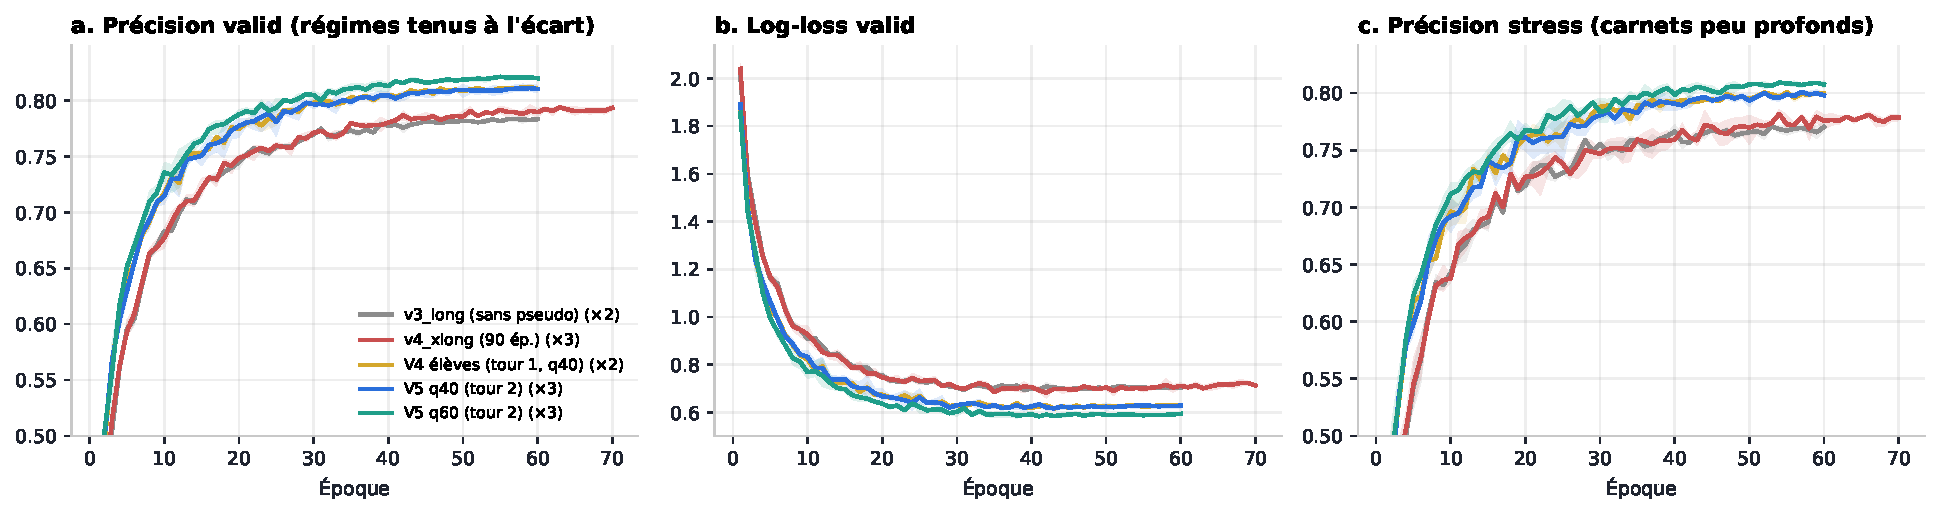
\includegraphics[width=\linewidth]{figures/v5_learning_curves_all.pdf}
\caption{Courbes d'apprentissage des trois générations (moyenne sur les graines ; bande = min/max). Les élèves des deux tours se séparent des modèles sans pseudo-labels dès les premières époques. Leur log-loss valid descend à 0,59--0,63 contre 0,70 et ne remonte pas. \code{v4\_xlong} rejoint \code{v3\_long} sans le dépasser nettement (la courbe s'arrête à 70 époques, l'arrêt précoce d'une graine).}
\label{fig:curves}\end{figure}

\begin{figure}[H]\centering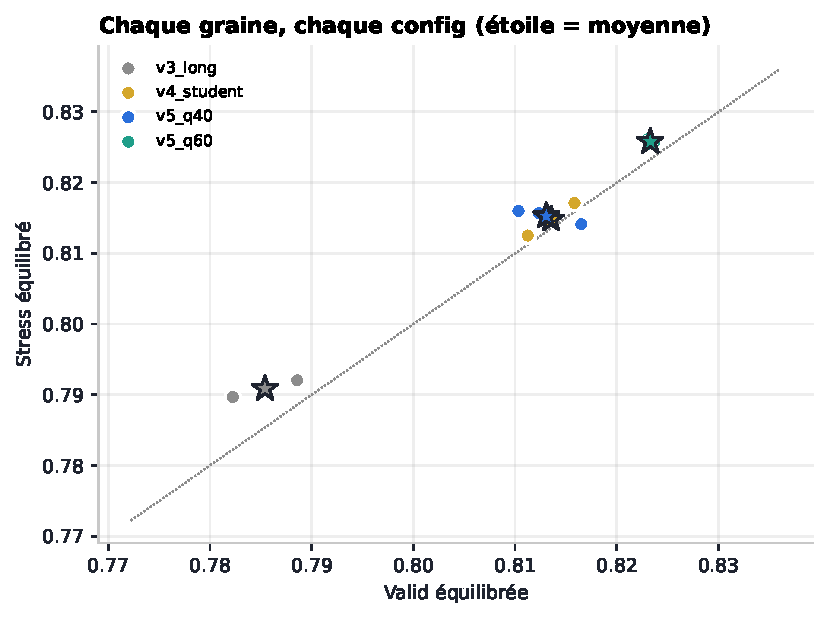
\includegraphics[width=.6\linewidth]{figures/v5_runs_all.pdf}
\caption{Chaque graine, en valid et en stress équilibrés. Les générations forment des grappes nettes, et la dispersion entre graines (moins de 0,5 point) est petite devant l'écart entre générations.}
\end{figure}

\paragraph{Ensemble et post-traitements.} L'alignement de profondeur n'apporte que $+0{,}2$ point en stress, sous le seuil de $+0{,}3$ fixé d'avance : il est rejeté, et $\gamma_{\text{test}}=1$ (contre 1,239 en V4). La cascade se lit sur le pool valid $\cup$ stress :
\begin{table}[H]\centering\small
\begin{tabular}{lcccc}
\toprule
Étape & V4 & V5 & $\Delta$ V5 vs V4\\
\midrule
Meilleur modèle seul & 0,808 & 0,818 & +1,0\\
Moyenne de l'ensemble & 0,830 & 0,842 & +1,2\\
+ Sinkhorn & 0,835 & 0,846 & +1,1\\
+ voisins (\code{combo}, $k=10$, $\alpha=0{,}5$, 5 it.) & 0,848 & 0,856 & +0,8\\
\midrule
Gain des voisins & +1,3 & +1,0 & \\
\bottomrule
\end{tabular}
\caption{Cascade interne (précision ; équilibrée à partir de Sinkhorn). Mesures contaminées : seule la forme de la cascade est informative.}
\end{table}
\noindent Les voisins rapportent moins en V5 : leurs pseudo-labels venaient d'un professeur déjà lissé, donc les élèves ont absorbé une partie de l'information du voisinage. La grille (figure~\ref{fig:nbr}) garde le même optimum qu'en V3 et V4 ($\alpha=0{,}5$, $k=10$), ce qui rend le passage à $k_{\text{test}}=40$ cohérent d'un tour à l'autre.

\begin{figure}[H]\centering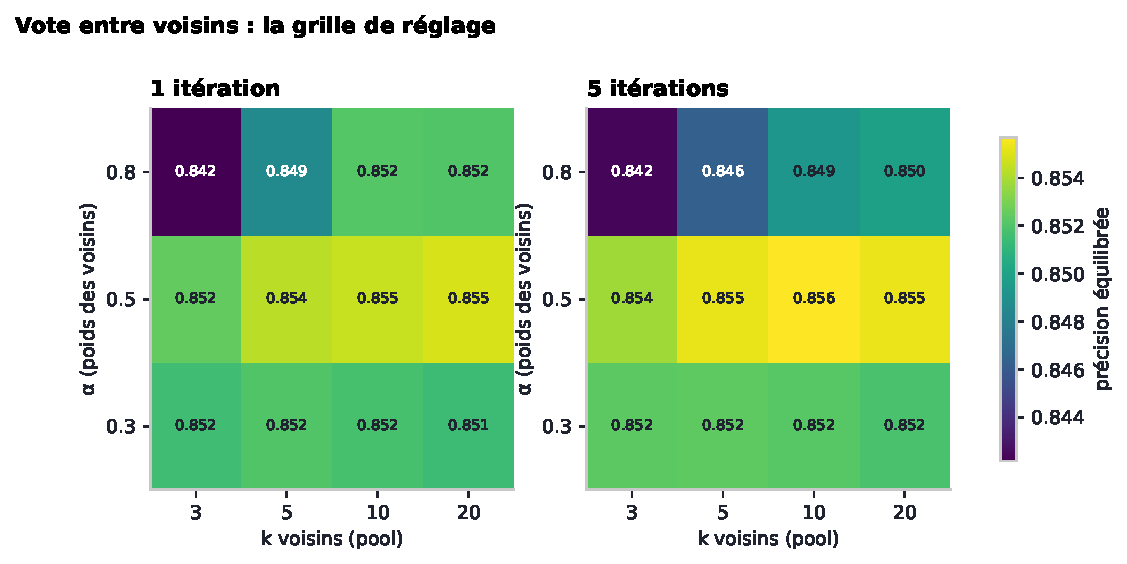
\includegraphics[width=.85\linewidth]{figures/v5_neighbours.pdf}
\caption{Grille du vote entre voisins sur le pool. Un $\alpha$ trop fort (0,8) dégrade d'autant plus que $k$ et le nombre d'itérations augmentent : le lissage écrase alors l'information propre à chaque fenêtre.}
\label{fig:nbr}\end{figure}

\subsection{Ce qui change au test, et le verdict du LB}
\begin{table}[H]\centering\small
\begin{tabular}{lccc}
\toprule
Soumission V5 & Différent de V4 C (total) & sur $\mathcal{S}_{0,6}$ (60\,\%) & hors $\mathcal{S}_{0,6}$ (40\,\%)\\
\midrule
ALL (6 élèves) & 11,2\,\% & 1,0\,\% & \textbf{26,5\,\%}\\
E (\code{v5\_q60} $\times3$) & 12,1\,\% & 0,8\,\% & 29,2\,\%\\
F (\code{v5\_q40} $\times3$) & 12,6\,\% & 2,0\,\% & 28,4\,\%\\
\bottomrule
\end{tabular}
\caption{Les élèves recopient le professeur là où ils ont été étiquetés, et modifient plus d'une fenêtre sur quatre ailleurs.}
\end{table}

\begin{figure}[H]\centering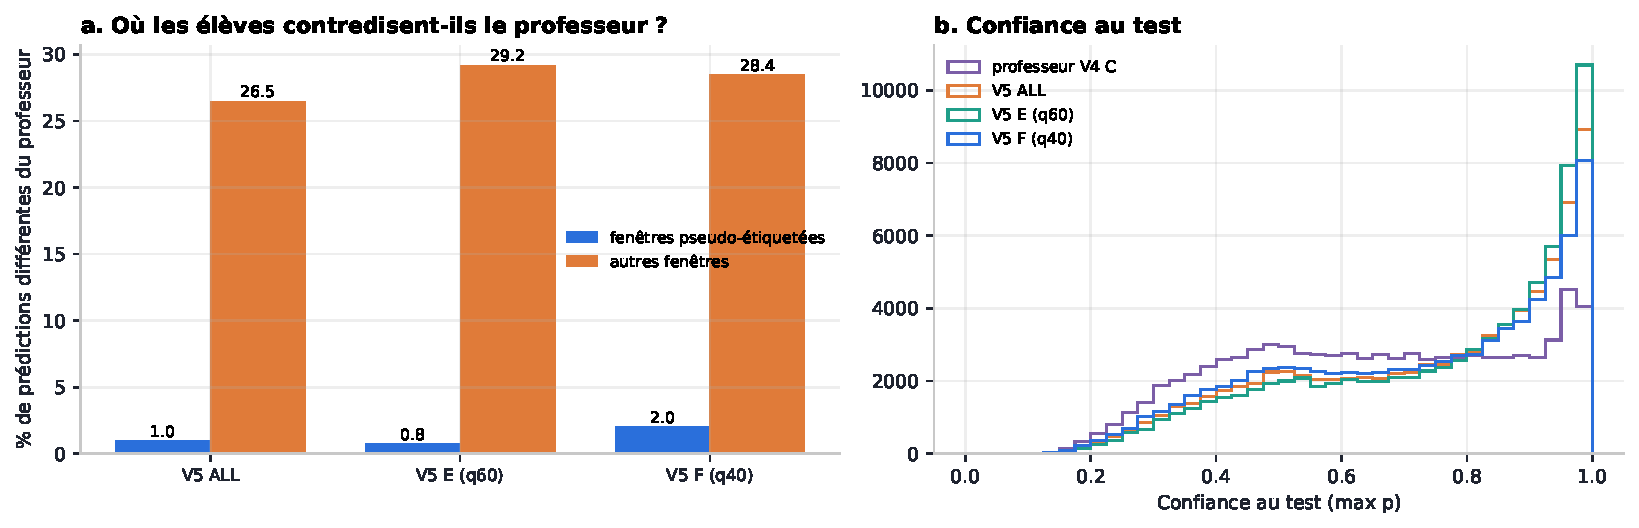
\includegraphics[width=\linewidth]{figures/v5_test_changes.pdf}
\caption{(a) Désaccords avec le professeur, sur et hors pseudo-labels. (b) Confiance au test. La masse du professeur, étalée entre 0,4 et 0,7, se concentre chez les élèves au-dessus de 0,9.}
\label{fig:testchg}\end{figure}

\begin{table}[H]\centering\small
\begin{tabular}{llc}
\toprule
Soumission & Contenu & LB public\\
\midrule
V4 C (professeur) & — & 0,6551\\
\textbf{V5 ALL} & 6 élèves, Sinkhorn, voisins ($k=40$) & \textbf{0,6835}\\
V5 E & \code{v5\_q60} $\times3$ seuls, mêmes post-traitements & 0,6822\\
V5 F & \code{v5\_q40} $\times3$ seuls & non soumise\\
\bottomrule
\end{tabular}
\caption{H1 est confirmée : $+2{,}8$ points sur le professeur. E fait presque aussi bien que ALL avec deux fois moins de modèles. H2 (E $-$ F) reste ouverte faute de soumission F.}
\end{table}

\paragraph{Le durcissement de la confiance n'est pas un mauvais calibrage.} La figure~\ref{fig:testchg}b est le symptôme classique du \emph{biais de confirmation}~\cite{arazo} : un élève entraîné sur ses propres certitudes devient plus sûr de lui. Mais sur le stress, les élèves sont \emph{mieux} calibrés que les modèles sans pseudo-labels (figure~\ref{fig:calib}, ECE de 0,027 à 0,006), et le LB a progressé. À ce tour, la confiance accrue est donc surtout justifiée. La réserve de la section~\ref{sec:contam} s'applique encore : le stress n'est pas indépendant des pseudo-labels.

\begin{figure}[H]\centering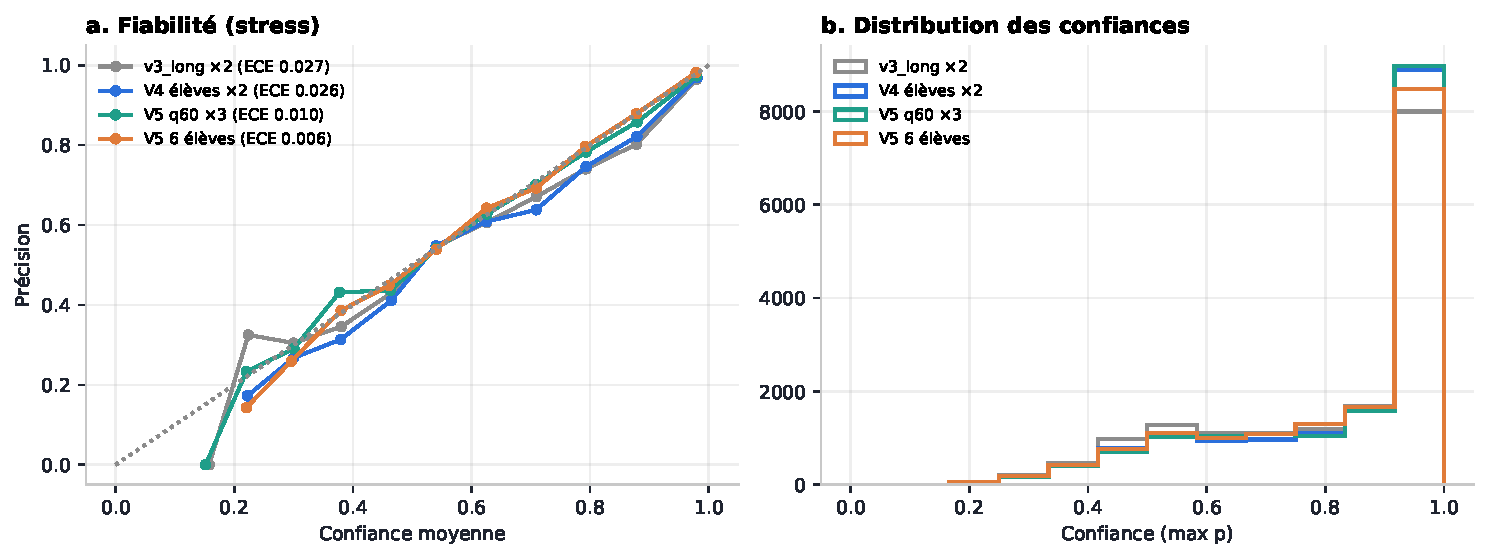
\includegraphics[width=\linewidth]{figures/v5_calibration_all.pdf}
\caption{Calibration sur le stress. (a) Courbes de fiabilité et erreur de calibration attendue (ECE, 12 classes de confiance). (b) Distribution des confiances.}
\label{fig:calib}\end{figure}

\subsection{Où se trouvent les erreurs restantes}
\begin{figure}[H]\centering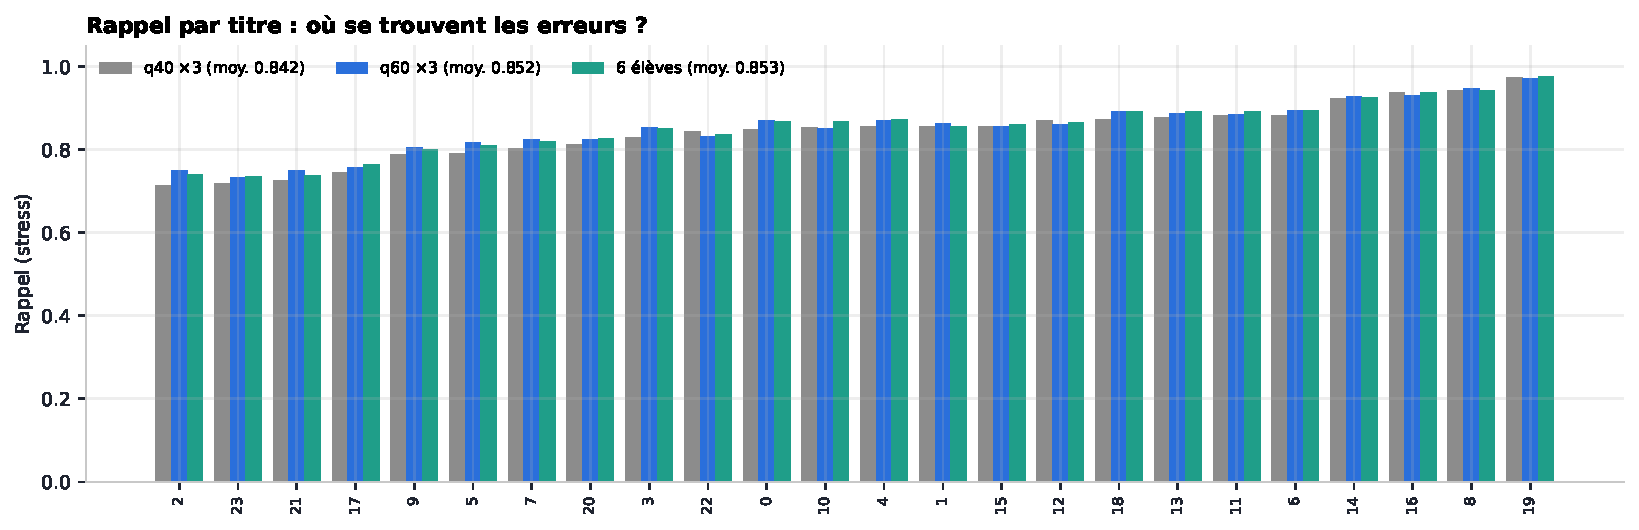
\includegraphics[width=\linewidth]{figures/v5_recall_by_class.pdf}
\caption{Rappel par titre sur le stress, pour les élèves q40, q60 et l'ensemble des 6, titres triés du plus difficile au plus facile.}
\end{figure}
\begin{figure}[H]\centering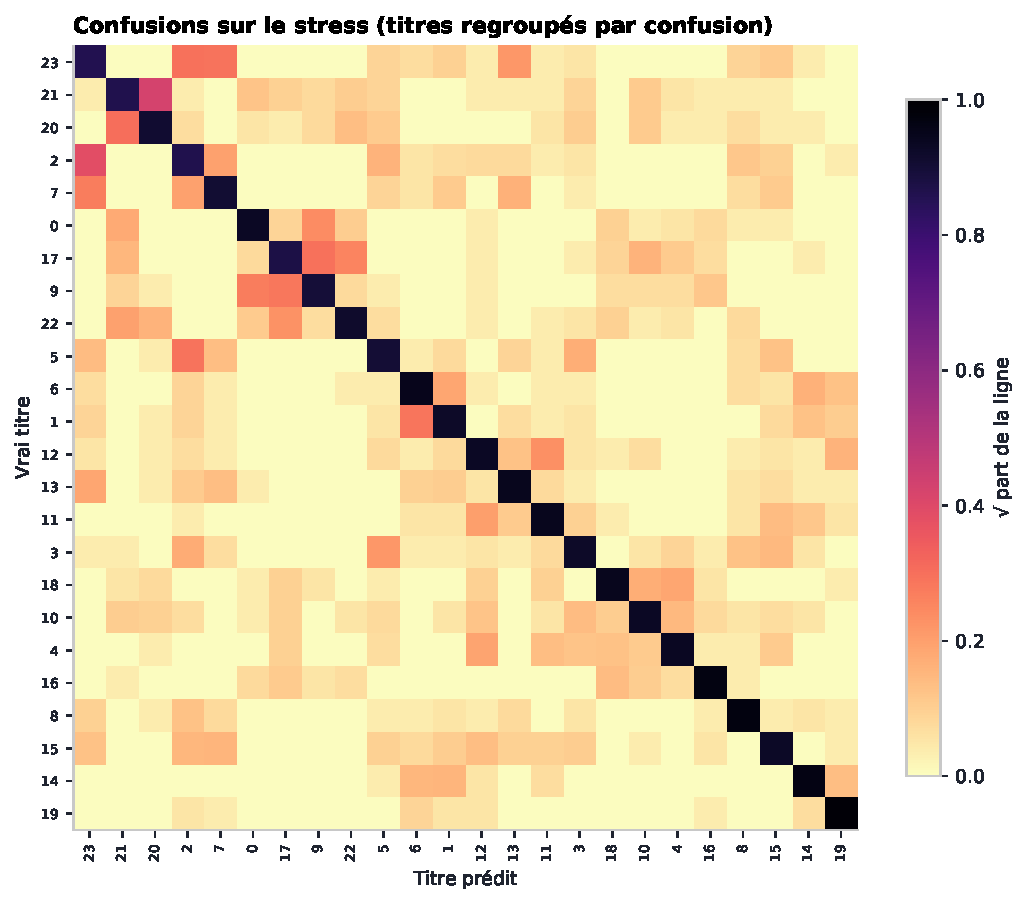
\includegraphics[width=.72\linewidth]{figures/v5_confusion.pdf}
\caption{Confusions de l'ensemble V5 sur le stress, avec les titres ordonnés par regroupement hiérarchique. Les erreurs ne sont pas diffuses : elles se concentrent dans quelques familles, notamment $\{20,21\}$, $\{2,7,23\}$, $\{0,9,17,22\}$ et $\{1,6\}$. À l'intérieur d'une famille, les titres partagent vraisemblablement un régime de tick et des conventions de lot proches (section~\ref{sec:unites}). La séparation demande alors des traits plus fins que la grille de prix.}
\label{fig:confusion}\end{figure}
\begin{figure}[H]\centering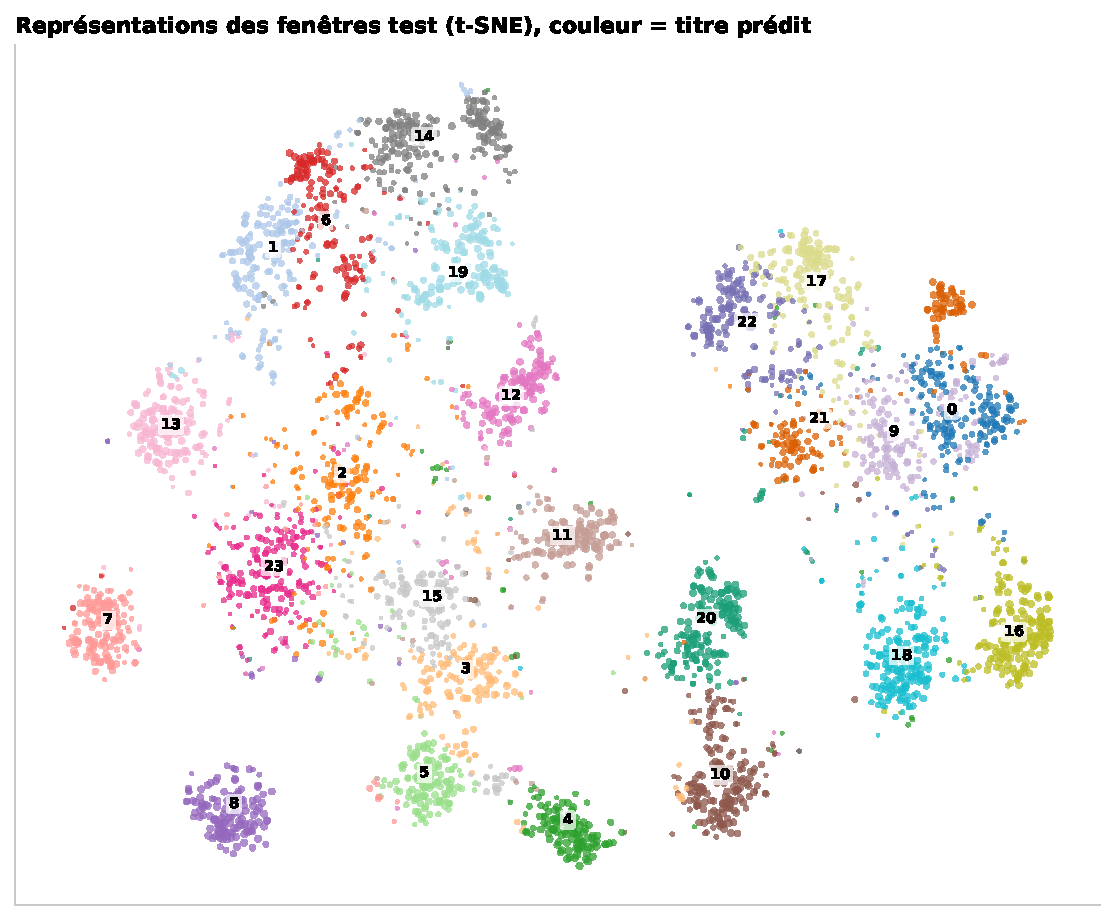
\includegraphics[width=.68\linewidth]{figures/v5_tsne_test.pdf}
\caption{Carte t-SNE de 4\,000 fenêtres test (représentations des élèves V5 refit), couleur = titre prédit, taille = confiance. Plusieurs titres forment des îlots isolés (7, 8, 13, 16). D'autres se touchent, et ce sont les mêmes familles que sur la matrice de confusion : $\{0,9,17,21,22\}$ à droite, $\{1,6,14,19\}$ en haut.}
\end{figure}

\subsection{Lecture d'ensemble}
\begin{enumerate}
\item \textbf{L'auto-apprentissage est le levier qui transfère le mieux.} Deux tours : $+2{,}0$ puis $+2{,}8$ points. Le second tour rapporte \emph{plus} que le premier, alors que son gain interne est plus petit ($+0{,}8$ point en stress équilibré). Les rendements ne décroissent pas encore.
\item \textbf{Les mesures internes sous-estiment tout ce qui exploite la période test.} C'était déjà le cas des voisins ($+1{,}3$ en interne, $+3{,}2$ au LB). Valid et stress appartiennent à la période d'entraînement : elles ne contiennent pas la direction du changement de période, qui est justement ce que les élèves apprennent.
\item \textbf{Le protocole de contrôle a été décisif.} Sans la soumission D, le $+2$ de la V4 aurait été attribué en partie aux 90 époques, qui en réalité \emph{coûtent} des points. Une soumission, une différence : c'est ce qui rend les conclusions défendables.
\item \textbf{Règle d'arrêt.} Le biais de confirmation grandit à chaque tour. Un troisième tour (professeur V5 ALL) n'est justifié que tant que le LB progresse. Le premier tour sans gain arrête la boucle.
\end{enumerate}

\section{Limites, menaces à la validité, suite}\label{sec:limites}

\subsection{Ce qui n'est pas établi}
\begin{enumerate}
\item \textbf{Attribution causale du gain.} Le passage de 0,5072 à 0,5700 mêle quatre changements : la représentation (unités, tokens, parcours d'ordres), l'architecture, l'ensemble de 4 modèles et le refit. Aucune soumission n'isole l'un d'eux. Le fait que \code{control\_gru}, qui reçoit les nouvelles entrées, dépasse nettement le GRU de R1 en validation suggère que la représentation pèse lourd. Mais la validation est biaisée.
\item \textbf{Validation non représentative.} Faute de dates, aucune partition ne tient des jours entiers à l'écart. Toutes les mesures internes sont optimistes. Les intervalles bootstrap sous-estiment la variance d'un facteur $\sqrt{\mathrm{deff}}$ inconnu.
\item \textbf{Leaderboard public.} Il est mesuré sur une partie du test, inconnue ici. Le consulter trop souvent ferait sur-apprendre ce sous-ensemble : \code{LEADERBOARD.md} limite et documente les soumissions.
\item \textbf{Hypothèse du prix.} « Prix plus élevés dans la période test » relie trois observations (profondeur, odd lots, lots ronds), mais le niveau de prix n'est pas observé.
\item \textbf{Transductivité.} Le sens du stress, l'équilibrage et le lissage par voisins utilisent les entrées test. Il faut vérifier que le règlement l'autorise. Dans le cas contraire, la soumission de référence est 0,5700.
\end{enumerate}

\subsection{Prochaines expériences}
\begin{center}\small
\begin{tabularx}{\linewidth}{>{\raggedright\arraybackslash}p{3.4cm}>{\raggedright\arraybackslash}X>{\raggedright\arraybackslash}p{3.8cm}}
\toprule
Expérience & Hypothèse & Abandon si\\
\midrule
V4 : pseudo-étiquetage & apprendre sur des fenêtres test étiquetées par V3 B (accord lissé/brut, quota par titre) adapte le modèle à la période & C\_k40 $\le$ D\_k40 au LB\\
V4 : 90 époques & l'entraînement n'était pas saturé à 60 & gain inférieur à l'écart entre graines\\
V4 : $k$ au test & $k=40$ n'est pas optimal & variantes à $\pm0{,}3$ pt de B\\
Token $D^{\text{pré}}_t$ (§\ref{sec:dpost}) & distinguer « où était l'ordre » de « ce qu'il a fait au carnet » & stress équilibré inchangé\\
SignatureLite & 3 convolutions + pooling (≈ 100\,k paramètres) suffisent, sans attention & écart > 0,5 pt vs \code{v3\_long}\\
Regroupement explicite en jours & voter par paquet de 20 fenêtres plutôt que par $k$ voisins & pas de gain sur B\\
\bottomrule
\end{tabularx}
\end{center}

\subsection{Conclusion}
Le gain le plus robuste de ce travail ne vient pas d'une couche de réseau. Il vient de trois décisions. D'abord, \emph{regarder} la donnée dans ses propres unités, ce qui a fait apparaître le régime de tick comme signature stable. Ensuite, \emph{refuser} de croire la validation aléatoire. Enfin, \emph{diagnostiquer le test sans labels} avant de le soumettre. L'équilibrage de Sinkhorn n'est qu'une conséquence de ce diagnostic : une projection entropique de deux lignes, dont la justification tient en une formule de Bayes.

\appendix
\section{Notation}
\begin{center}\small
\begin{tabular}{ll}
\toprule
Symbole & Signification\\
\midrule
$K=24$, $L=100$ & nombre de titres, événements par fenêtre\\
$\tick=0{,}01$, $\lot=100$ & tick, lot\\
$v_t,o_t,a_t,s_t,\tau_t$ & venue, ordre, action, côté, trade\\
$p_t,b_t,\alpha_t$ & prix de l'ordre, meilleur bid, meilleur ask (recentrés)\\
$q^b_t,q^a_t,Q_t,I_t$ & tailles aux meilleures limites, profondeur, imbalance\\
$f_t,F_t$ & flux, flux en lots\\
$S_t,h_t,D_t$ & spread en ticks, $\Delta$mid en demi-ticks, distance au meilleur prix de son côté\\
$\rho(t),n_t,g_t,a^{\leftarrow}_t,a^\circ_t,N_t$ & rang d'ordre, occurrence, écart, action précédente, première action, taille du parcours\\
$s^\star,d^\star,f^\star$ & médianes positives locales (spread, profondeur, $|f|$)\\
$\pi_k(W)$ & part du temps à $k$ ticks de spread\\
$d=96$, $H=4$, $d_h=24$ & largeur, têtes, largeur par tête\\
$S_{ij}$, $\beta_h$ & indicatrice « même ordre », biais appris de la tête $h$\\
$P,\bar P,Q^\star$ & probabilités d'un modèle, du blend, après Sinkhorn\\
$u_i,w_k$ & facteurs de ligne et de classe (Sinkhorn)\\
$A,\alpha,k$ & graphe des voisins, poids de propagation, nombre de voisins\\
\bottomrule
\end{tabular}
\end{center}

\section{Hyperparamètres}
\begin{center}\small
\begin{tabular}{ll}
\toprule
Élément & Valeur (\code{configs/base.json})\\
\midrule
Split & audit 10\,\%, stress 10\,\% (queue \code{auto}), valid 15\,\%, seed 42\\
Screening & XGBoost, base \code{base\_relative}+\code{cat\_freq}, 50\,\% du fit, seed 0\\
SignatureNet & $d=96$, $H=4$, 2 conv, 2 attentions, contexte 64, dropout 0,15\\
Entraînement & lot de 512, AdamW $10^{-3}$, wd 0,01, warmup 1 époque, cosinus, 40 époques, patience 8\\
Perte & entropie croisée, lissage 0,02, écrêtage du gradient 1\\
Augmentations (robust) & venue 0,1 ; blocs 0,1 ; jitter de niveaux 0,25\\
Augmentation (depthaug) & $\sigma_d=0{,}3$\\
Refit & budget \code{epochs}\\
Sinkhorn & 50 itérations, cible uniforme, écrêtage $10^{-12}$\\
Voisins & $k\in\{3,5,10,20\}$, $\alpha\in\{0{,}3;0{,}5;0{,}8\}$, 1 ou 5 itérations, $k_{\text{test}}=4k$\\
\bottomrule
\end{tabular}
\end{center}

\section{Contrats testés (\code{tests/test\_lab.py}, 15 tests)}
\begin{enumerate}
\item labels alignés par \code{obs\_id} même si \code{y\_train} est mélangé ;
\item fenêtres non contiguës refusées ;
\item rang d'ordre invariant par renumérotation bijective ; identifiants manquants jamais égaux ;
\item helpers de parcours d'ordre égaux à une boucle naïve ;
\item unités en ticks sur une fenêtre construite à la main ;
\item \code{base\_relative} invariant à l'échelle des tailles, \code{levels} sensible ;
\item cache de blocs indexé par le contexte $(\tick,\lot)$ ;
\item partitions disjointes et complètes, 24 classes partout, audit indépendant du réglage du stress ;
\item tabulaire de bout en bout, prédictions test alignées (accuracy > hasard sur le synthétique) ;
\item réseau : reprise identique, configuration différente refusée, refit, cinq encodeurs ;
\item augmentation de profondeur, extraction de représentations, refus d'utiliser les poids du refit sur des partitions étiquetées ;
\item la mise à l'échelle ne touche que les canaux de profondeur et conserve $q^b/q^a$ ;
\item le lissage par voisins corrige des erreurs isolées ; le voisinage exclut la fenêtre elle-même ;
\item les indicateurs sans labels sont nuls sur des prédictions équilibrées ;
\item Sinkhorn : lignes de somme 1, colonnes de somme $N/K$.
\end{enumerate}

\section{Reproduire}
\begin{verbatim}
pip install -r requirements.txt
python scripts/kaggle_upload.py --notes "..."      # code -> Dataset Kaggle privé
# Kaggle : CFM_Signature_Lab.ipynb (round 1) puis CFM_Round2.ipynb
python tests/test_lab.py                            # 15 contrats, CPU
python -m cfm neural --config configs/signature.json --name sig_s0 --refit epochs
python -m cfm blend --runs sig_s0 sig_s1 --submit --balance
\end{verbatim}
\noindent Pour le run 1, les fichiers \code{runs/*/result.json}, \code{history.csv}, les probabilités \code{*.npz} et \code{ledger.csv} se trouvent dans \code{lab\_results.zip}.


\begin{thebibliography}{9}
\bibitem{saerens} M.~Saerens, P.~Latinne, C.~Decaestecker. \emph{Adjusting the outputs of a classifier to new a priori probabilities: a simple procedure}. Neural Computation, 14(1), 2002.
\bibitem{cuturi} M.~Cuturi. \emph{Sinkhorn distances: lightspeed computation of optimal transport}. NeurIPS, 2013.
\bibitem{sinkhorn} R.~Sinkhorn, P.~Knopp. \emph{Concerning nonnegative matrices and doubly stochastic matrices}. Pacific Journal of Mathematics, 21(2), 1967.
\bibitem{cks} R.~Cont, A.~Kukanov, S.~Stoikov. \emph{The price impact of order book events}. Journal of Financial Econometrics, 12(1), 2014. arXiv:1011.6402.
\bibitem{vaswani} A.~Vaswani et al. \emph{Attention is all you need}. NeurIPS, 2017.
\bibitem{shaw} P.~Shaw, J.~Uszkoreit, A.~Vaswani. \emph{Self-attention with relative position representations}. NAACL, 2018.
\bibitem{loshchilov} I.~Loshchilov, F.~Hutter. \emph{Decoupled weight decay regularization}. ICLR, 2019.
\bibitem{zhou} D.~Zhou, O.~Bousquet, T.~N.~Lal, J.~Weston, B.~Schölkopf. \emph{Learning with local and global consistency}. NIPS, 2003.
\bibitem{lee} D.-H.~Lee. \emph{Pseudo-label: the simple and efficient semi-supervised learning method for deep neural networks}. ICML Workshop on Challenges in Representation Learning, 2013.
\bibitem{xie} Q.~Xie, M.-T.~Luong, E.~Hovy, Q.~V.~Le. \emph{Self-training with Noisy Student improves ImageNet classification}. CVPR, 2020.
\bibitem{arazo} E.~Arazo, D.~Ortego, P.~Albert, N.~E.~O'Connor, K.~McGuinness. \emph{Pseudo-labeling and confirmation bias in deep semi-supervised learning}. IJCNN, 2020.
\bibitem{blum} A.~Blum, T.~Mitchell. \emph{Combining labeled and unlabeled data with co-training}. COLT, 1998.
\bibitem{lipton} Z.~Lipton, Y.-X.~Wang, A.~Smola. \emph{Detecting and correcting for label shift with black box predictors}. ICML, 2018.
\end{thebibliography}
\end{document}
